% Template LaTeX file for DAFx-20 papers
%
% To generate the correct references using BibTeX, run
%     latex, bibtex, latex, latex
% modified...
% - from DAFx-00 to DAFx-02 by Florian Keiler, 2002-07-08
% - from DAFx-03 to DAFx-04 by Gianpaolo Evangelista, 2004-02-07 
% - from DAFx-05 to DAFx-06 by Vincent Verfaille, 2006-02-05
% - from DAFx-06 to DAFx-07 by Vincent Verfaille, 2007-01-05
%                          and Sylvain Marchand, 2007-01-31
% - from DAFx-07 to DAFx-08 by Henri Penttinen, 2007-12-12
%                          and Jyri Pakarinen 2008-01-28
% - from DAFx-08 to DAFx-09 by Giorgio Prandi, Fabio Antonacci 2008-10-03
% - from DAFx-09 to DAFx-10 by Hannes Pomberger 2010-02-01
% - from DAFx-10 to DAFx-12 by Jez Wells 2011
% - from DAFx-12 to DAFx-14 by Sascha Disch 2013
% - from DAFx-15 to DAFx-16 by Pavel Rajmic 2015
% - from DAFx-16 to DAFx-17 by Brian Hamilton 2016
% - from DAFx-17 to DAFx-18 by Annibal Ferreira and Matthew Davies 2017
% - from DAFx-18 to DAFx-19 by Dave Moffat 2019
% - from DAFx-19 to DAFx-20 by Gianpaolo Evangelista 2019
%
% Template with hyper-references (links) active after conversion to pdf
% (with the distiller) or if compiled with pdflatex.
%
% 20060205: added package 'hypcap' to correct hyperlinks to figures and tables
%                      use of \papertitle and \paperauthorA, etc for same title in PDF and Metadata
% 20190205: Package 'hypcap' removed, and replaced with 'caption', to allow for the inclusion
%			of a CC UP licence.
%
% 1) Please compile using latex or pdflatex.
% 2) If using pdflatex, you need your figures in a file format other than eps! e.g. png or jpg is working
% 3) Please use "paperftitle" and "pdfauthor" definitions below

%------------------------------------------------------------------------------------------
%  !  !  !  !  !  !  !  !  !  !  !  ! user defined variables  !  !  !  !  !  !  !  !  !  !  !  !  !  !
% Please use the following commands to define title and author(s) of the paper.
% paperauthorA MUST be the the first author of the paper
% Please comment the unused definitions 
\def\papertitle{Room Impulse Response Estimation using Signed Distance Functons}
\def\paperauthorA{Patrik Lechner}
\def\paperauthorB{Author Two}
\def\paperauthorC{Author Three}
\def\paperauthorD{Author Four}
%\def\paperauthorE{Author Five}
%\def\paperauthorF{Author Six}
%\def\paperauthorG{Author Seven}
%\def\paperauthorH{Author Eight}
%\def\paperauthorI{Author Nine}
%\def\paperauthorJ{Author Ten}

% Authors' affiliations have to be set below

%------------------------------------------------------------------------------------------
\documentclass[twoside,a4paper]{article}
\usepackage{etoolbox}
\usepackage{dafx_20}
\usepackage{amsmath,amssymb,amsfonts,amsthm}
\usepackage{euscript}
%\usepackage[latin1]{inputenc}
\usepackage[T1]{fontenc}
\usepackage[utf8]{inputenc}
%\usepackage[T1]{fontenc}
%\usepackage{lmodern}
\usepackage{nimbusserif}
\usepackage{ifpdf}
\usepackage[english]{babel}
\usepackage{caption}
% \usepackage{subfig} % or can use subcaption package
\usepackage{color}

\input glyphtounicode
\pdfgentounicode=1

\setcounter{page}{1}
\ninept

% build the list of authors and set the flag \multipleauth to handle the et al. in the copyright note (in DAFx_20.sty)
%==============================DO NOT MODIFY =======================================
\newcounter{numauth}\setcounter{numauth}{1}
\newcounter{listcnt}\setcounter{listcnt}{1}
\newcommand\authcnt[1]{\ifdefined#1 \stepcounter{numauth} \fi}

\newcommand\addauth[1]{
\ifdefined#1 
\stepcounter{listcnt}
\ifnum \value{listcnt}<\value{numauth}
\appto\authorslist{, #1}
\else
\appto\authorslist{~and~#1}
\fi
\fi}
%======DO NOT MODIFY UNLESS YOUR PAPER HAS MORE THAN 10 AUTHORS========================
%==we count the authors defined at the beginning of the file (paperauthorA is mandatory and already accounted for)
\authcnt{\paperauthorB}
\authcnt{\paperauthorC}
\authcnt{\paperauthorD}
\authcnt{\paperauthorE}
\authcnt{\paperauthorF}
\authcnt{\paperauthorG}
\authcnt{\paperauthorH}
\authcnt{\paperauthorI}
\authcnt{\paperauthorJ}
%==we create a list of authors for pdf tagging, for example: paperauthorA, paperauthorB, ... and paperauthorF (last author)
\def\authorslist{\paperauthorA}
\addauth{\paperauthorB}
\addauth{\paperauthorC}
\addauth{\paperauthorD}
\addauth{\paperauthorE}
\addauth{\paperauthorF}
\addauth{\paperauthorG}
\addauth{\paperauthorH}
\addauth{\paperauthorI}
\addauth{\paperauthorJ}
%====================================================================================

\usepackage{times}
% Saves a lot of ouptut space in PDF... after conversion with the distiller
% Delete if you cannot get PS fonts working on your system.


% pdf-tex settings: detect automatically if run by latex or pdflatex
\newif\ifpdf
\ifx\pdfoutput\relax
\else
   \ifcase\pdfoutput
      \pdffalse
   \else
      \pdftrue
\fi

\ifpdf % compiling with pdflatex
  \usepackage[pdftex,
    pdftitle={\papertitle},
    pdfauthor={\authorslist},
    pdfsubject={Proceedings of the 23rd International Conference on Digital Audio Effects (DAFx-20)},
    colorlinks=false, % links are activated as color boxes instead of color text
    bookmarksnumbered, % use section numbers with bookmarks
    pdfstartview=XYZ % start with zoom=100% instead of full screen; especially useful if working with a big screen :-)
  ]{hyperref}
  \pdfcompresslevel=9
  \usepackage[pdftex]{graphicx}
 % \usepackage[figure,table]{hypcap}
\else % compiling with latex
  \usepackage[dvips]{epsfig,graphicx}
  \usepackage[dvips,
    pdftitle={\papertitle},
    pdfauthor={\authorslist},
    pdfsubject={Proceedings of the 23rd International Conference on Digital Audio Effects (DAFx-20)},
    colorlinks=false, % no color links
    bookmarksnumbered, % use section numbers with bookmarks
    pdfstartview=XYZ % start with zoom=100% instead of full screen
  ]{hyperref}
  % hyperrefs are active in the pdf file after conversion
  %\usepackage[figure,table]{hypcap}
\fi
\usepackage[hypcap=true]{caption}
\title{\papertitle}

% -------------SINGLE-AFFILIATION SINGLE-AUTHOR HEADER STARTS (uncomment below if your paper has a single author)----------------------------------------
\affiliation{
\paperauthorA\,\sthanks{Thanks to the predecessors for the templates}}
{\href{https://www.mdw.ac.at/ike/}{Institute 1} \\ University of Applied Sciences St.Poelten\\ St.Poelten, Austria\\
{\tt \href{mailto:dafx2020@gmail.com}{ptrk.lechner@gmail.com}}
}
%-------------SINGLE-AFFILIATION SINGLE-AUTHOR HEADER ENDS-------------------------------------------------------------------------------------------------------------------

%------------SINGLE-AFFILIATION MULTIPLE-AUTHORS HEADER STARTS (uncomment below if your paper has two or more authors from the same institution)
% \affiliation{
% \paperauthorA\,\sthanks{Thanks to the predecessors for the templates}and \paperauthorB \,\sthanks{This work was supported by the XYZ Foundation}}
% {\href{https://www.mdw.ac.at/ike/}{Institute 1} \\ University of Music and Performing Arts\\ Vienna, Austria\\
% {\tt \href{mailto:dafx2020@gmail.com}{dafx2020@gmail.com}}
% }
%-----------------------------------SINGLE-AFFILIATION-MULTIPLE-AUTHORS HEADER ENDS----------------------------------------------------------------------------------------

%---------------TWO-AFFILIATIONS HEADER STARTS (uncomment below if your paper has two authors, each from a different institution)-----------------------------
%\twoaffiliations{
%\paperauthorA \,\sthanks{Thanks to the predecessors for the templates}}
%{\href{https://www.mdw.ac.at/ike/}{Institute 1} \\ University of Music and Performing Arts\\ Vienna, Austria\\
%{\tt \href{mailto:dafx2020@gmail.com}{dafx2020@gmail.com}}
%}
%{\paperauthorB \,\sthanks{This work was supported by the XYZ Foundation}}
%{\href{http://dafx2019.bcu.ac.uk/}{Digital Media Technology Lab} \\ Birmingham City University \\ Birmingham, UK \\ {\tt \href{mailto:dafx2019@gmail.com}{dafx2019@gmail.com}}
%}
%-------------------------------------TWO-AFFILIATIONS HEADER ENDS------------------------------------------------------

%%---------------THREE-AFFILIATIONS HEADER STARTS (uncomment below if your paper has three authors, each from a different institution)-----------------------
%\threeaffiliations{
%\paperauthorA \,\sthanks{Thanks to the predecessors for the templates}}
%{\href{https://www.mdw.ac.at/ike/}{Institute 1} \\ University of Music and Performing Arts\\ Vienna, Austria\\
%{\tt \href{mailto:dafx2020@gmail.com}{dafx2020@gmail.com}}
%}
%{\paperauthorB \,\sthanks{This work was supported by the XYZ Foundation}}
%{\href{http://dafx2019.bcu.ac.uk/}{Digital Media Technology Lab} \\ Birmingham City University \\ Birmingham, UK \\ {\tt \href{mailto:dafx2019@gmail.com}{dafx2019@gmail.com}}
%}
%{\paperauthorC \,\sthanks{Illustrious contributor}}
%{\href{http://dafx2018.web.ua.pt/}{IEETA} \\ University of Aveiro \\ Aveiro, Portugal \\ {\tt \href{mailto:dafx2018_papers@ua.pt}{dafx2018\_papers@ua.pt}}
%}
%-------------------------------------THREE-AFFILIATIONS HEADER ENDS------------------------------------------------------

%----------------FOUR-AFFILIATIONS HEADER STARTS (uncomment below if your paper has four authors, , each from a different institution)-----------------------
% \fouraffiliations{
% \paperauthorA \,\sthanks{Thanks to the predecessors for the templates}}
% {\href{https://www.mdw.ac.at/ike/}{Institute 1} \\ University of Music and Performing Arts\\ Vienna, Austria\\
% {\tt \href{mailto:dafx2020@gmail.com}{dafx2020@gmail.com}}
% }
% {\paperauthorB \,\sthanks{This work was supported by the XYZ Foundation}}
% {\href{http://dafx2019.bcu.ac.uk/}{Digital Media Technology Lab} \\ Birmingham City University \\ Birmingham, UK \\ {\tt \href{mailto:dafx2019@gmail.com}{dafx2019@gmail.com}}
% }
% {\paperauthorC \,\sthanks{Illustrious contributor}}
% {\href{http://dafx2018.web.ua.pt/}{IEETA} \\ University of Aveiro \\ Aveiro, Portugal \\ {\tt \href{mailto:dafx2018_papers@ua.pt}{dafx2018\_papers@ua.pt}}
% }
% {\paperauthorD \,\sthanks{This guy is a very good fellow}}
% {\href{http://www.acoustics.ed.ac.uk}{Acoustics and Audio Group} \\ University of Edinburgh\\ Edinburgh, UK\\ {\tt \href{mailto:dafx17@ed.ac.uk}{dafx17@ed.ac.uk}}
% }
%-------------------------------------FOUR-AFFILIATIONS HEADER ENDS------------------------------------------------------



% ============MY ADDITIONS ====================


\usepackage{pgf}
% -----------plotting with tikz-------
\usepackage{tikz}
\usepackage[utf8]{inputenc}
% \usepackage{fontspec}  % optional
\usepackage{pgfplots}
\pgfplotsset{compat=newest}
\usepgfplotslibrary{groupplots}
\usepgfplotslibrary{dateplot}

% \usepgfplotslibrary{external} 
% \tikzexternalize
% ------------------------------------

% code
\usepackage{listings}
\lstset
{
frame = single,
}
% \lstset
% { %Formatting for code in appendix
%     % language=Matlab,
%     % basicstyle=\footnotesize,
%     numbers=left,
%     stepnumber=1,
%     showstringspaces=false,
%     tabsize=1,
%     breaklines=true,
%     breakatwhitespace=false,
% }

% subfigures (side by side)
\usepackage{subcaption}
% \usepackage{subfig}




% =============== BlockDiagram Drawing Config
\usetikzlibrary{shapes,arrows}
  \usetikzlibrary{trees, backgrounds}

% Definition of blocks:
\tikzset{%
  block/.style    = {draw, thick, rectangle, minimum height = 3em,
    minimum width = 3em},
  sum/.style      = {draw, circle, node distance = 2cm}, % Adder
  input/.style    = {coordinate}, % Input
  output/.style   = {coordinate}, % Output
  mult/.style   = {draw, isosceles triangle, minimum height=1cm, minimum width =1cm}
}
% mult/.style   = {isosceles triangle, sharp corners, anchor=center, xshift=-4mm, minimum height=1.5cm, minimum width =0.05cm}
%isosceles triangle, fill=gray!25, minimum width=1.5cm

% Defining string as labels of certain blocks.
\newcommand{\suma}{\Large$+$}
\newcommand{\inte}{$\displaystyle \int$}
\newcommand{\derv}{\huge$\frac{d}{dt}$}
\newcommand{\conv}{\huge$\ast$}

% ==

% ====================================






\begin{document}
% more pdf-tex settings:
\ifpdf % used graphic file format for pdflatex
  \DeclareGraphicsExtensions{.png,.jpg,.pdf}
\else  % used graphic file format for latex
  \DeclareGraphicsExtensions{.eps}
\fi

%\makeatletter
%\pdfbookmark[0]{\@pdftitle}{title}
%\makeatother

\maketitle

\begin{abstract}

Several algorithms and approaches for Room Impulse Response (RIR) estimation exist. To the best of the authors knowledge, there is no documentation of accuracy, speed or even the feasibility of using signed distance functions (SDFs) in combination with sphere tracing for this task. Here, a proof of concept with a focus on real-time performance is presented, that lacks many features such as frequency dependent absorption and scattering coefficients, arbitrary source and receiver directives etc. The results are shown and compared to real room impulse responses recorded by \cite{brinkmann_round_2019} and to a different simulation algorithm \cite{lehmann_fast_2020}. The implementation happens mostly inside a compute shader, an example application is provided in the framework \texttt{TouchDesigner}.\ 

The application as well as all generated data and \texttt{Jupyter Notebooks} can be found on this project's github repository\

 \href{https://github.com/hrtlacek/rayMarchReverb}{github.com/hrtlacek/rayMarchReverb}.
\end{abstract}

\section{Introduction}
\label{sec:intro}
Sphere tracing as defined by \cite{hart_sphere_1996} is used extensively in the so called "demo scene" to render 3D video demos via shaders in real time for decades. 
Sphere tracing is a version of the ray casting algorithm \cite{roth_ray_1982}. It relies on the geometry being defined as so called signed distance functions (SDFs), and does not directly support the import of standard 3D Polygonal geometry or meshes. One of the advantages lies in the algorithm's potential improved speed in comparison to fixed-step ray casting. SDFs are used to describe implicit surfaces, typically via a function $f : \mathbb{R}^3 \rightarrow \mathbb{R}$(although in principle, arbitrary dimensions are possible, $f : \mathbb{R}^n \rightarrow \mathbb{R}$, see Section \ref{sec:concl}). This function should be designed to return a negative value if the locus of the point is inside the geometry, a positive value if outside and 0 if on the surface to define the desired geometry. Additionally it is advantageous to design this function in a way so it is lipschitz continuous. If $f$ is defined carefully, the distance to the nearest surface is returned by this function and therefore always known during stepping along a view-ray. 
Since the distance to the nearest surface is always known, the step size of a ray tracing algorithm can be dynamically adjusted, see Figure \ref{sphereViz}, resulting in fewer iterations along a ray, and therefore in significant speedups. 

\begin{figure}[ht]
\centerline{\includegraphics[scale=0.5]{img/sphereTracingViz.png}}
\caption{\label{sphereViz}{\it Visualization of the sphere tracing algorithm in 2D. A ray is sent from the source (left) to the right until it hits a surface, always moving the maximum distance as the SDF informs the tracing algorithm about the distance to nearest surface.}}
\end{figure}

\subsection{Previous Work}
\label{ssec:prev}
A lot of previous work exists both in the field of Ray/sphere tracing and RIR estimation.
As shown in \cite{alpkocak_computing_2010} and \cite{brinkmann_round_2019} there are numerous approaches for estimating RIRs. Besides Ray-based methods such as the "Image Source Method", Ray-tracing and hybrid approaches, wave-based methods such as Finite Differences are becoming increasingly interesting due to advancements in computation power and research. Still, wave-based methods seem to be too slow for real-time applications. With the Pascal Architecture, NVIDIA introduced real-time ray tracing done on the GPU with NVIDIA VRWorks™ Audio \cite{noauthor_vrworks_nodate}.

% NVIDIA is working in the field of real time ray traced audio simulation
% NVIDIA VRWorks™ Audio (introduced with the Pascal GPU architecture) 



% \subsubsection*{RIR Estimation}
% \cite{alpkocak_computing_2010} gives an overview of methods in use for RIR estimation.


\subsubsection*{Sphere Tracing}
Sphere tracing itself was first described by \cite{hart_sphere_1996}. Many authors since then described improvements in speed e.g. \cite{balint_accelerating_2018} or the addition of features such as \cite{quilez_inigo_nodate}, \cite{keinert_enhanced_2014} or the activity of the \href{www.shadertoy.com}{shadertoy.com}-community.
Defining SDFs is an active field of research and there are several projects that aim at easier construction of SDFs and integration in 3D frameworks such as \href{https://github.com/Flafla2/Generic-Raymarch-Unity}{https://github.com/Flafla2/Generic-Raymarch-Unity} and \cite{lechner_hrtlacektdraymarchtoolkit_2020}.



\subsection{Motivation}
\label{subs:mot}
The reasons why sphere tracing in a compute shader for RIR estimation has not been documented until now probably lie in the relatively new introduction of compute shaders as well as in the difficulty of creating SDFs(in comparison to using existing 3D /CAD models and import them to polygon based ray tracers).
\subsubsection{Sphere tracing}
As described above, ray tracing in general is in use. Sphere tracing has a number of advantages over ray tracing polygonal surfaces. It is "procedural" by default, since all geometry is defined by implicit surface equations. More over sphere tracing approximates cone tracing for reducing aliasing artifacts in the pixel domain\cite{hart_sphere_1996}, which in the audio domain, is considered to have advantages but is very time confusing in a non-SDF setup\cite{alpkocak_computing_2010}. The deformation and rounding of geometry is possible in a very efficient way, which might offer an opportunity to approximate low-frequency response due to diffraction artifacts. Since geometry is not defined via vertizes and edges, there is no such thing as increasing the complexity of a shape in this way. Rounding a geometrical shape is a mere subtraction since it just shifts the rendering to another iso-surface, which is getting increasingly smooth as shown in \ref{sdf_2d_box}. Depending on the construction of the geometry, this way, holes and cavities (such as in a diffusor) can also be made disappear for a low-frequency pass as shown in figure \ref{fig:diffSmooth}.

\begin{figure}[ht]
\centerline{\includegraphics[scale=0.6]{img/sdf2dbox.png}}
\caption{\label{sdf_2d_box}{\it rounding the box given in Equation \ref{eq:eq1} by subtraction of $0.7$. Visible iso-lines (gray) are generated by the distance function. The subtraction shifts the surface to a different, more round, iso-line.}}
\end{figure}  


\begin{figure}[ht]
\centering
\begin{subfigure}[t]{0.2\textwidth}
  \centering
  \includegraphics[width=0.9\linewidth]{img/diffusorNorm.png}
  \caption{\it Diffusor shape}
  \label{fig:diffNorm}
\end{subfigure}%
\begin{subfigure}[t]{0.2\textwidth}
  \centering
  \includegraphics[width=0.9\linewidth]{img/diffusorSmooth.png}
  \caption{\it After subtraction: rounded and closed.}
  \label{fig:sub2}
\end{subfigure}
\caption{\it The diffusor from scene 1 in \cite{brinkmann_round_2019} was reconstructed exactly(a). A subtraction of $0.01$ from the distance function causes the holes to close(b).}
\label{fig:diffSmooth}
\end{figure}

\subsubsection{Implementation}
It is possible to implement the chosen algorithm on the CPU and the GPU. A number of frameworks could be chosen for GPU accelerated computation such as OpenCL or NVIDIA CUDA. For example \cite{stoltzfus_performance_2017} gives an overview of GPU development environments suitable for RIR estimation. The choice of a shader has the advantage of being more operating system independent and hardware independent as for example the use of CUDA ties to NVIDIA GPUs. Compute shaders (in contrast to fragment shaders) make it possible to write to arbitrary output locations which is necessary for generating the actual impulse response from the measurement of timings. Since they are available since OpenGL 4.3 (August 2012) / OpenGL ES 3.1 they are both aged enough to have received broad support in other frameworks and relatively new in respect to first publications about sphere tracing. Another reason for the choice of compute shaders is their simplicity. In comparison to CUDA and OpenCL, shaders are easier to write and the use of the Graphics Library Shading Language (GLSL) is widespread. Achieving the whole computation, from the definition of the geometry, to the ray tracing up until the actual impulse response computation in a single shader makes this attempt highly portable and expandable.

\section{Generation of SDFs}

Only rather simplistic shapes where needed for this proof-of-concept. Mostly boxes are used and combined in various ways to achieve reflection areas, shoe-box scenes and the little more complex diffusor shape of scene 1 in \cite{brinkmann_round_2019}. A simple 3D box SDF with a size of $R_x$x$R_y$x$R_z$ can be described by:

\begin{equation}
  f(p_x, p_y, p_z) = \sqrt{c_0(p_x - R_x)^2 + c_0(p_y - R_y)^2 + c_0(p_z - R_z)^2}
  \label{eq:eq1}
\end{equation}

where $c_0$ is just clipping at 0:

\begin{equation}
c_0(x) = max(x,0) 
\end{equation}

which translates to GLSL conveniently:

\begin{lstlisting}[language=C, caption={\it GLSL code for creating a box SDF},captionpos=b, label=lst:boxSdf]
float box(vec3 pos, vec3 R){
    return length(max(abs(pos) - R,0));
}
\end{lstlisting}

\cite{hart_sphere_1996} gives a list mathematical definitions of many shapes and for example \href{http://mercury.sexy/hg_sdf/}{http://mercury.sexy/hg\_sdf/} provides a rich and advanced library of shapes and operators that are ready to use for creation of more complex scenery.


\section{Sphere Tracing}
For simplicity, deterministic equal-angle Ray Tracing is used in contrast to Monte Carlo or Equal Area Ray tracing (EART) \cite{gu_room_2014}. Unidirectional ray tracing has been used, also for simplicity reasons, although \cite{cao_interactive_2016} has shown that bidirectional ray tracing offers advantages. Since the classical sphere tracing algorithm was adapted, it was found to be simplest to consider the "camera" to be the receiver/microphone as it would receive light. It sends out rays that might hit the sound source, which acts as a receiver of rays. The sound source is chosen to be a sphere. Choosing a correct volume for the receiver is critical and using a constant size can introduce systematic errors \cite{xiangyang_accuracy_2003}, \cite{alpkocak_computing_2010}. A number of models are available to compute the receiver Volume, $V_r$. Typically factors such as room volume, number of rays and the distance from source are used for this computation. 
As in \cite{brandao_ray_nodate}, \cite{alpkocak_computing_2010}, and \cite{dalenback_room_1996} the receiver was allowed to grow in volume. While \cite{brandao_ray_nodate} and \cite{dalenback_room_1996} use time as a factor to let the receiver grow, in this attempt the reflection count, $k$ is used. Initially when a ray is sent, $k=1$ and when it hits a surface, this counter is increased by one so the source grows by this factor for this particular ray. So instead of using time, the model provided in \cite{alpkocak_computing_2010} is used and augmented with the $k$ term:
\begin{equation}
V_r = k \omega d_{SR}\sqrt{\frac{4}{N}}
\end{equation}
with 
\begin{equation}
\omega = log_{10}{V_{room}}
\end{equation}
where $d_{SR}$ is the source-receiver distance, $N$ is the number of initial rays and $V_{room}$ is the volume of the room.\

The actual sphere tracing largely follows the original formulation in \cite{hart_sphere_1996} and is implemented as:

% \begin{equation}
% t_{i+1} = t_i + F(t_i)
% \end{equation}
% With $t_{i}$  being the current distance travelled along the ray being used in combination with the evaluation of the distance function $F()$ 
Here, this is implemented in the following way:
\begin{lstlisting}[language=C, caption={\it GLSL pseudo code for sphere tracing},captionpos=b,label=lst:sphereTrace]
for (i=0;i++;i<imax){
  vec3 pos = ro + t*rd;
  Sdf res = map(pos);
  t += res.x;
  if(res.x<epsilon){
    break
  }
}
\end{lstlisting} 

In the above simplified code listing, \texttt{ro} is a \texttt{vec3} that defines the ray origin, \texttt{rd} the ray direction and \texttt{epsilon} can be set to adjust the algorithms precision. The \texttt{map()} function in this case not only returns the distance computed via the SDF(\texttt{res.x}) but a \texttt{struct} that can contain material properties (reflection coefficients etc.). Here it was used to distinguish between a sound source and a regular reflective body.
The space is sampled spherically and \texttt{rd} is generated from the compute shader's \texttt{gl\_GlobalInvocationID}.
From there, the space is sampled using the following very simplified pseudo code:
\begin{lstlisting}[language=C, caption={\it GLSL pseudo code for sampling the space and writing to the RIR.},captionpos=b, label=lst:mainloop]
Sdf res = castRay(ro,rd)
for (int k=0;k<numReflections;k++;){
  if(ComingFromReflectiveBdy){
    rd = relect(rd,normal);
  }
  res = castRay(ro,rd);
  t = res.x;
  pos = ro+rd*t;
  if(res.body == soundSource){
    travelDistance+=t;
    readWrite(travelDistance,k);
  }
}

\end{lstlisting}

Here, \texttt{castRay()} refers to a function that looks similar to the sphere tracing function above and \texttt{readWrite()} refers to a function that takes the total distance a ray has travelled from source to receiver including all reflections and the number of reflections. From the distance it computes the location where to write to in the impulse response and the attenuation. It then reads the current value at this location and adds the corresponding value, making use of a compute shader's capability to read and write it's output and write to arbitrary output locations. The necessity to write to arbitrary output locations is the main reason for choosing a compute shader over a fragment shader. But it is possible to define most of the functionality to in one file that is included to a compute shader to calculate the RIR and to a fragment shader for visualization. This is particularly handy during construction of geometry.


\begin{figure}[ht]
\center
\begin{tikzpicture}

\node (lib) at (0,0) [rectangle,draw] {$F(p_{xyz})$};
\node (frag) at (-2,-1) [rectangle,draw] {$fragment\ shader$};
\node (comp) at (2,-1) [rectangle,draw] {$compute\ shader$};
\draw node [block, below of=frag, node distance = 1.5cm](rend){\includegraphics[width=.1\textwidth]{img/diffusorNorm.png}};
\draw node [block, below of=comp, node distance = 1.5cm](H){$H(n)$};

\draw[->] (lib) -- node {} (frag);
\draw[->] (lib) -- node {} (comp);
\draw[->] (frag) -- node {}(rend);
\draw[->] (comp) -- node {}(H);



\end{tikzpicture}
\caption{\label{fig:bd_shaders}{\it A lot of the code, especially the map function, $F(p_{xyz})$, which contains the SDF can be shared between a fragment shader used for visualization and a compute shader responsible for RIR calculation.}}
\end{figure}



\begin{enumerate}
\item reflection
\item low frequency pass
\end{enumerate}


\section{impulse response Generation}
The room is assumed to be a linear time invariant (LTI) system. Due to the proof-of-concept nature of this proposal, a highly simplified model for RIR computation is used. Sphere tracing delivers distances and number of reflections for $M$ rays in this implementation. Each ray follows a number of reflections $K(m)$. Each reflection pass adds up to a total travel distance of the ray, $d(m)$. The sound source is assumed to send out a discrete impulse, the kronecker delta function, $\delta(n)$. As non-integer delays are ignored in this implementation, the shader will just write to the rounded integer delay location $\tau_s$ in the impulse response, $H(n)$,that corresponds to the distance:
\begin{equation}
H(n) = \sum_{m=0}^M \delta(n-\tau_s(m))\cdot \alpha(m)\cdot -1^{K(m)}
\end{equation}
The total attenuation per ray $\alpha(m)$ can be computed by using a material dependent coefficient of reflection $\alpha_{mat}$ that is stored in the \texttt{Sdf struct}. At each reflection pass $k$ this results in a possibly different reflection pass dependent coefficient $\alpha_{mat}(k,m)$ and keeping a running product in the loop of Listing \ref{lst:mainloop}:
\begin{equation}
\alpha(m)=\prod_{k=0}^{K(m)} \alpha_{mat}(k,m)
\end{equation}
For simplicity's sake, here only one global coefficient $\alpha_G$ is implemented resulting in:
\begin{equation}
\alpha(m) = \alpha_G^{K(m)}
\end{equation}

Additionally, a proof-of-concept for frequency dependent loss for each reflection is introduced into the model. As a computationally efficient heuristic, binomial filter is used \cite{aubury_binomial_1996}, \cite{derpanis_overview_nodate}. A simple one-zero filter $G(z)$ is applied at each reflection:

\begin{equation}
G(z,K) = (1+z^{-1})^K \cdot \frac{1}{2}^K
\end{equation}
The advantage of using such a simple filter is that a $K$-stage cascade's impulse response can be computed easily without applying the filter repeatedly. By doing the discrete time inverse fourier transform of the transfer function $G(z)$ the $N$-length impulse response is obtained:

\begin{equation}
  G(n,K) = \mathfrak{F}^{-1}\{ G(z) \} = (\frac{1}{2})^K \frac{1}{N}  \sum_{\omega = 0}^\pi (1+e^{-j\omega})^{K} e^{j\omega n} 
\end{equation}
A binomial filter's impulse response converges to a gaussian bell curve which can be approximated as:

\begin{equation}
G(n,K) \approx  \frac{1}{\sigma \cdot \sqrt{2 \pi}} \cdot e ^{-\frac{1}{2} (\frac{n-\mu}{\sigma})^2}
\label{eq:assump}
\end{equation}


with 

\begin{equation}
\sigma = \sqrt{K 0.231 + 0.562}
\end{equation}
and 
\begin{equation}
\mu = \frac{K}{2} + \frac{1}{2}
\end{equation}

The right hand side of Equation \ref{eq:assump} is simply the normal distribution, which is computationally efficient to calculate for any $K$.

So instead of adding $\delta(n-\tau(m))$ into the IR, simply $G(n-\tau(m),K)$ is used. 
Similar to many other implementations, a high-pass filter is applied to the resulting RIR to compensate for low-frequency components resulting mainly from the spacial extendedness of the sound receiver shape.



\begin{figure*}[ht]
    \center
    \begin{subfigure}[t]{0.45\textwidth}
      \centering
      % This file was created by tikzplotlib v0.9.1.
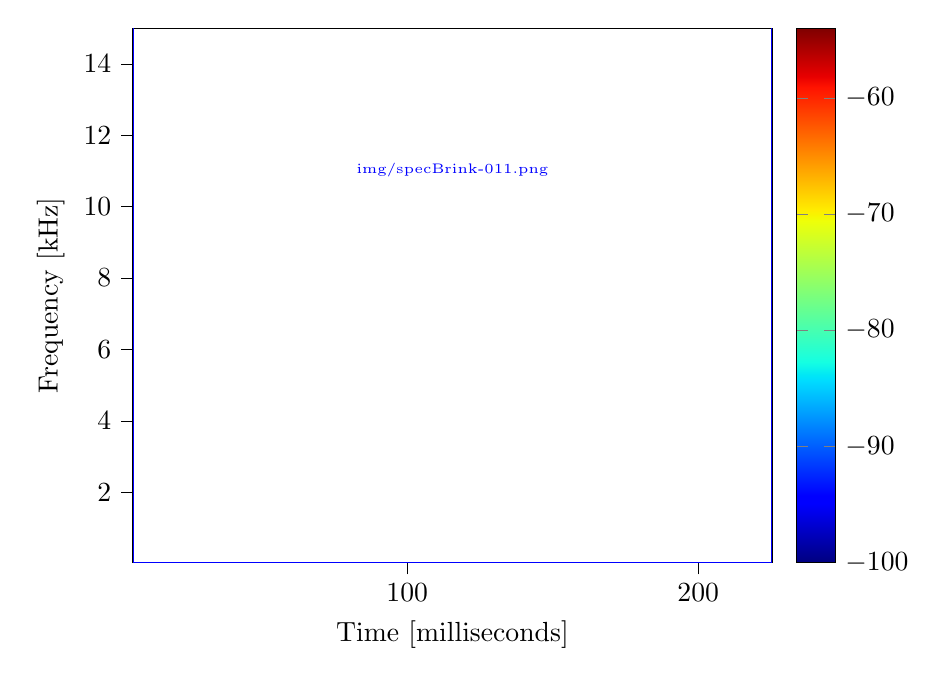
\begin{tikzpicture}

\begin{axis}[
colorbar,
colorbar style={ylabel={}, y label style={yshift=1.5em}},
colormap={mymap}{[1pt]
  rgb(0pt)=(0.0000,0.0000,0.5000);
  rgb(22pt)=(0.0000,0.0000,1.0000);
  rgb(25pt)=(0.0000,0.0000,1.0000);
  rgb(68pt)=(0.0000,0.8600,1.0000);
  rgb(70pt)=(0.0000,0.9000,0.9677);
  rgb(75pt)=(0.0806,1.0000,0.8871);
  rgb(128pt)=(0.9355,1.0000,0.0323);
  rgb(130pt)=(0.9677,0.9630,0.0000);
  rgb(132pt)=(1.0000,0.9259,0.0000);
  rgb(178pt)=(1.0000,0.0741,0.0000);
  rgb(182pt)=(0.9091,0.0000,0.0000);
  rgb(200pt)=(0.5000,0.0000,0.0000)
},
point meta max=-54.0062,
point meta min=-100.0000,
tick align=outside,
tick pos=left,
width=0.8\textwidth,
x grid style={white!69.0196!black},
xlabel={Time [milliseconds]},
xmin=0005.7, xmax=225.4,xtick={0, 100,200},
xtick style={color=black},
y grid style={white!69.0196!black},
ylabel={Frequency [kHz]},
ymin=0.0300000, ymax=15.0000000,
ytick style={color=black}
]
\addplot graphics [includegraphics cmd=\pgfimage,xmin=5.7, xmax=225.4, ymin=0.0000, ymax=22.0500000] {img/specBrink-011.png};
\end{axis}

\end{tikzpicture}

    \caption{\label{fig:fig:multReflSpecOrig} \it Original recording, scene 1, multiple reflections from \cite{brinkmann_round_2019}. }
    \end{subfigure}% 
    \begin{subfigure}[t]{0.45\textwidth}
      \centering
      % This file was created by tikzplotlib v0.9.1.
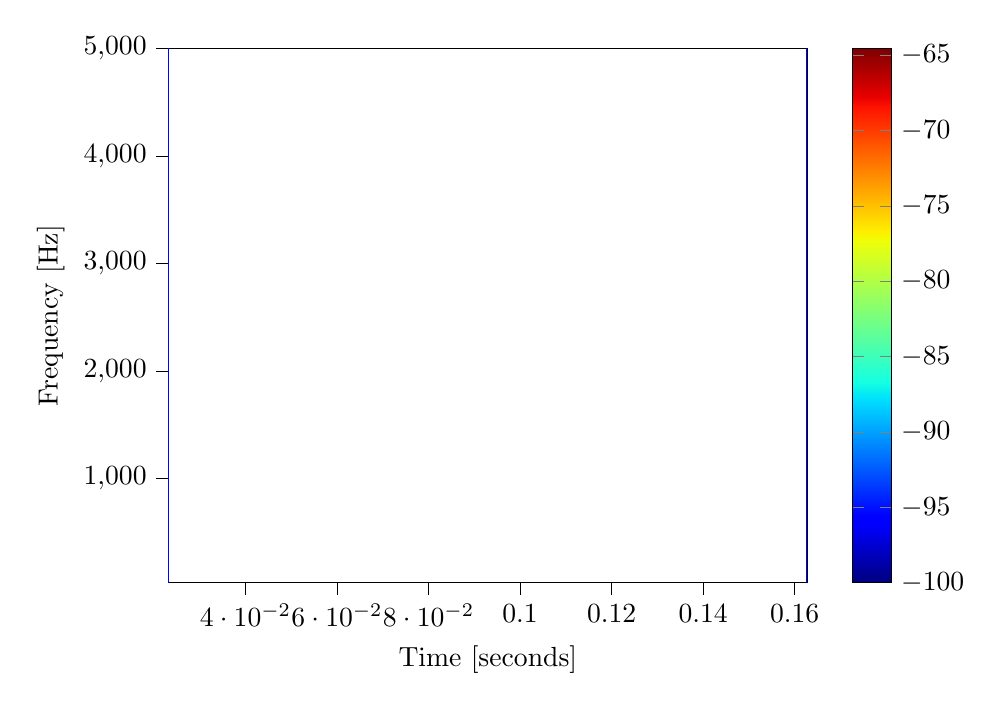
\begin{tikzpicture}

\begin{axis}[
colorbar,
colorbar style={ylabel={}},
colormap={mymap}{[1pt]
  rgb(0pt)=(0.0000,0.0000,0.5000);
  rgb(22pt)=(0.0000,0.0000,1.0000);
  rgb(25pt)=(0.0000,0.0000,1.0000);
  rgb(68pt)=(0.0000,0.8600,1.0000);
  rgb(70pt)=(0.0000,0.9000,0.9677);
  rgb(75pt)=(0.0806,1.0000,0.8871);
  rgb(128pt)=(0.9355,1.0000,0.0323);
  rgb(130pt)=(0.9677,0.9630,0.0000);
  rgb(132pt)=(1.0000,0.9259,0.0000);
  rgb(178pt)=(1.0000,0.0741,0.0000);
  rgb(182pt)=(0.9091,0.0000,0.0000);
  rgb(200pt)=(0.5000,0.0000,0.0000)
},
point meta max=-64.5644,
point meta min=-100.0000,
tick align=outside,
tick pos=left,
width=0.8\textwidth,
x grid style={white!69.0196!black},
xlabel={Time [seconds]},
xmin=0.0231, xmax=0.1628,
xtick style={color=black},
y grid style={white!69.0196!black},
ylabel={Frequency [Hz]},
ymin=30.0000, ymax=5000.0000,
ytick style={color=black}
]
\addplot graphics [includegraphics cmd=\pgfimage,xmin=0.0231, xmax=0.1628, ymin=0.0000, ymax=22050.0000] {img/simBrink-007.png};
\end{axis}

\end{tikzpicture}

      \caption{\label{fig:multReflSpecSim} \it Simulated using the proposed method. }
    \end{subfigure}
    \caption{\it Comparison of spectra of a real impulse response (a) and the proposed method (b).}
    \label{fig:multReflSpecCompare}
\end{figure*}


\section{Results}

\begin{figure*}[ht]
    \center
    \begin{subfigure}[t]{0.45\textwidth}
      \centering
      % This file was created by tikzplotlib v0.9.1.
\begin{tikzpicture}

\begin{axis}[
colorbar,
colorbar style={ylabel={}},
colormap={mymap}{[1pt]
  rgb(0pt)=(0.0000,0.0000,0.5000);
  rgb(22pt)=(0.0000,0.0000,1.0000);
  rgb(25pt)=(0.0000,0.0000,1.0000);
  rgb(68pt)=(0.0000,0.8600,1.0000);
  rgb(70pt)=(0.0000,0.9000,0.9677);
  rgb(75pt)=(0.0806,1.0000,0.8871);
  rgb(128pt)=(0.9355,1.0000,0.0323);
  rgb(130pt)=(0.9677,0.9630,0.0000);
  rgb(132pt)=(1.0000,0.9259,0.0000);
  rgb(178pt)=(1.0000,0.0741,0.0000);
  rgb(182pt)=(0.9091,0.0000,0.0000);
  rgb(200pt)=(0.5000,0.0000,0.0000)
},
point meta max=-54.1665,
point meta min=-100.0000,
tick align=outside,
tick pos=left,
width=0.8\textwidth,
x grid style={white!69.0196!black},
xlabel={Time [milliseconds]},
xmin=23.1, xmax=72.1,xtick={30,40,50,60,70},
xtick style={color=black},
y grid style={white!69.0196!black},
ylabel={Frequency [kHz]},
ymin=0.0300000, ymax=5.0000000,
ytick style={color=black}
]
\addplot graphics [includegraphics cmd=\pgfimage,xmin=23.1, xmax=72.1, ymin=0.0000, ymax=22.0500000] {img/shoebox_orig-002.png};
\end{axis}

\end{tikzpicture}

    \caption{\label{fig:shoe} \it Spec by matlab. }
    \end{subfigure}% 
    \begin{subfigure}[t]{0.45\textwidth}
      \centering
      \input{img/shoebox_sim}
      \caption{\label{fig:shoe} \it Simulated. }
    \end{subfigure}
    \caption{\it Impulse response of shoebox room. Computed using the proposed method and \cite{lehmann_fast_2020}.}
    \label{fig:test}
\end{figure*}


All of the following results have been computed with 10 reflection passes, and $1024^2$ rays. The computations were made on a strong consumer-grade machine (Intel i7 CPU, NVIDIA Geforce 1080ti). The computation time for simple scenes such as scene 1, rigid in \cite{brinkmann_round_2019} was at $<\frac{1}{60}$ seconds including the computation of a simple visualization in real time. The most complex scenes(geometrically and in regards to the amount of reflections) that where tested, the shoebox scene and scene 1 with added diffusor, where computed in less than $<\frac{1}{50}$ seconds. As expected, the method therefore outperforms CPU based methods in computation time.  \

The results are compared to a different simulation using the image source method \cite{lehmann_fast_2020} and \cite{brinkmann_round_2019} who generated a dataset featuring recordings in in an anechoic chamber with simple shapes. Note that for the comparison with \cite{brinkmann_round_2019} in figure \ref{fig:multRefl} ignores the frequency response of the speaker and microphone that was used in the original recording. As can be seen in the plot, the original recording features visible amount of difference to an ideal impulse even with the direct signal. 

Since this implementation lacks of features such as material-specific reflection coefficients and passes for multiple octave bands, it is not possible to accurately compare previous work with the proposed method by simply using the same materials. It can be shown that by adjusting reflection coefficients, the method can be matched up with existing work.

\begin{figure}

    \begin{center}
      \input{img/brink}
    \end{center}
    
    \caption{\label{fig:multRefl} \it RIR computed using the proposed method and measured by \cite{brinkmann_round_2019}, scene 3, multiple reflection at opposed MDF plates.}
\end{figure}

\begin{figure}
    \begin{center}
      \input{img/brinkDiff}
    \end{center}
    
    \caption{\label{fig:diffuser} \it RIR computed using the proposed method and measured by \cite{brinkmann_round_2019}, scene 1, a single reflection with a diffuser.}
\end{figure}


The shoebox scene features a small room with dimensions 3 x 4 x 2.5 meters. Note that \cite{lehmann_fast_2020} used a sampling rate of 16kHz and has been upsampled to 44.1 kHz for comparison reasons. This probably led to the pre-ringing artifacts present in Figure \ref{fig:shoe}.

\begin{figure}
    \begin{center}
      % This file was created by tikzplotlib v0.9.1.
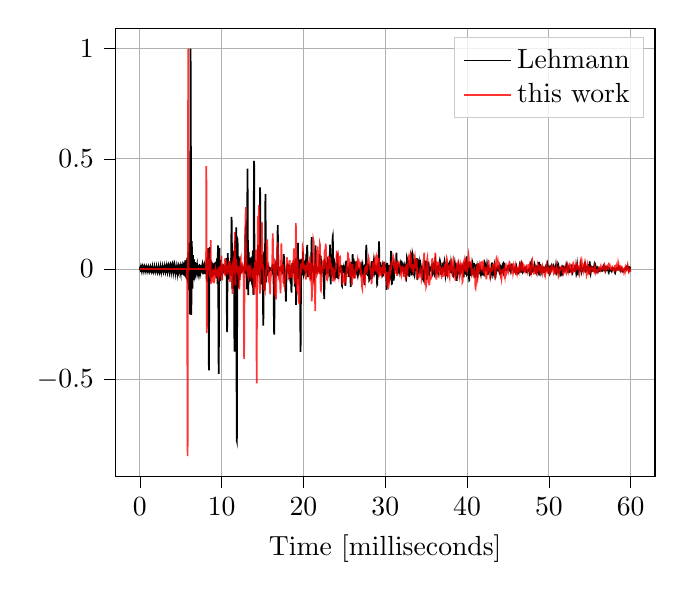
\begin{tikzpicture}

\begin{axis}[
legend cell align={left},
legend style={fill opacity=0.8, draw opacity=1, text opacity=1, draw=white!80.00000!black},
tick align=outside,
tick pos=left,
x grid style={white!69.01961!black},
xlabel={Time [milliseconds]},
xmajorgrids,
xmin=-3.00, xmax=62.98,
xtick style={color=black},
y grid style={white!69.01961!black},
ymajorgrids,
ymin=-0.94115, ymax=1.09244,
ytick style={color=black}
]
\addplot [semithick, black]
table {%
0.0 -0.00417
0.02 0.00715
0.05 0.00938
0.06999999999999999 0.00061
0.09000000000000001 -0.00894
0.11 -0.00852
0.13999999999999999 0.00107
0.16 0.00872
0.18000000000000002 0.00576
0.2 -0.00420
0.23 -0.00964
0.25 -0.00441
0.27 0.00533
0.29 0.00832
0.32 0.00121
0.34 -0.00768
0.36000000000000004 -0.00810
0.39 0.00035
0.41 0.00784
0.43 0.00572
0.45 -0.00348
0.48000000000000004 -0.00907
0.5 -0.00461
0.5199999999999999 0.00467
0.54 0.00800
0.57 0.00156
0.5900000000000001 -0.00714
0.61 -0.00801
0.63 -0.00006
0.66 0.00744
0.68 0.00579
0.7 -0.00305
0.73 -0.00881
0.75 -0.00480
0.7699999999999999 0.00429
0.79 0.00790
0.82 0.00183
0.8400000000000001 -0.00684
0.86 -0.00803
0.88 -0.00036
0.91 0.00724
0.93 0.00592
0.95 -0.00278
0.98 -0.00873
1.0 -0.00500
1.02 0.00407
1.0399999999999998 0.00792
1.07 0.00206
1.09 -0.00670
1.11 -0.00815
1.13 -0.00058
1.16 0.00721
1.1800000000000002 0.00611
1.2 -0.00261
1.22 -0.00881
1.25 -0.00522
1.27 0.00401
1.2899999999999998 0.00812
1.32 0.00226
1.34 -0.00679
1.36 -0.00844
1.38 -0.00068
1.41 0.00751
1.4300000000000002 0.00648
1.45 -0.00281
1.47 -0.00976
1.5 -0.00634
1.52 0.00364
1.5399999999999998 0.00880
1.56 0.00330
1.59 -0.00643
1.61 -0.00914
1.63 -0.00174
1.66 0.00716
1.6800000000000002 0.00723
1.7 -0.00157
1.72 -0.00901
1.75 -0.00645
1.77 0.00312
1.79 0.00857
1.81 0.00355
1.84 -0.00608
1.86 -0.00912
1.88 -0.00202
1.9 0.00695
1.9300000000000002 0.00735
1.95 -0.00131
1.97 -0.00894
2.0 -0.00664
2.02 0.00292
2.04 0.00861
2.06 0.00378
2.09 -0.00597
2.11 -0.00927
2.13 -0.00223
2.15 0.00695
2.18 0.00756
2.2 -0.00116
2.22 -0.00906
2.2399999999999998 -0.00688
2.27 0.00287
2.29 0.00884
2.31 0.00400
2.34 -0.00606
2.3600000000000003 -0.00958
2.3800000000000003 -0.00237
2.4 0.00721
2.4299999999999997 0.00793
2.4499999999999997 -0.00118
2.4699999999999998 -0.00955
2.49 -0.00726
2.52 0.00328
2.54 0.01001
2.56 0.00507
2.59 -0.00599
2.61 -0.01051
2.63 -0.00335
2.65 0.00717
2.68 0.00885
2.7 -0.00024
2.72 -0.00954
2.7399999999999998 -0.00821
2.77 0.00220
2.79 0.00958
2.81 0.00531
2.83 -0.00566
2.8600000000000003 -0.01054
2.8800000000000003 -0.00361
2.9 0.00709
2.9299999999999997 0.00906
2.9499999999999997 -0.00006
2.97 -0.00966
2.99 -0.00849
3.02 0.00216
3.04 0.00987
3.0599999999999996 0.00557
3.0799999999999996 -0.00582
3.11 -0.01099
3.13 -0.00376
3.15 0.00753
3.17 0.00963
3.2 -0.00020
3.22 -0.01075
3.2399999999999998 -0.00977
3.27 0.00178
3.29 0.01068
3.31 0.00670
3.33 -0.00554
3.3600000000000003 -0.01182
3.3800000000000003 -0.00481
3.4 0.00735
3.42 0.01047
3.4499999999999997 0.00088
3.47 -0.01029
3.49 -0.00996
3.5100000000000002 0.00157
3.54 0.01087
3.5599999999999996 0.00699
3.58 -0.00565
3.61 -0.01228
3.63 -0.00501
3.65 0.00781
3.67 0.01113
3.7 0.00077
3.72 -0.01147
3.7399999999999998 -0.01135
3.76 0.00122
3.79 0.01182
3.81 0.00819
3.83 -0.00549
3.85 -0.01330
3.8800000000000003 -0.00607
3.9 0.00786
3.92 0.01220
3.95 0.00172
3.9699999999999998 -0.01145
3.9899999999999998 -0.01179
4.01 0.00142
4.04 0.01303
4.0600000000000005 0.00945
4.08 -0.00541
4.1000000000000005 -0.01445
4.13 -0.00714
4.15 0.00806
4.17 0.01344
4.2 0.00258
4.22 -0.01192
4.24 -0.01305
4.26 0.00074
4.29 0.01341
4.31 0.00992
4.33 -0.00605
4.35 -0.01606
4.38 -0.00823
4.4 0.00864
4.42 0.01501
4.44 0.00332
4.47 -0.01295
4.49 -0.01467
4.51 0.00056
4.54 0.01526
4.56 0.01216
4.58 -0.00547
4.6 -0.01730
4.63 -0.00940
4.6499999999999995 0.00923
4.67 0.01678
4.6899999999999995 0.00401
4.720000000000001 -0.01456
4.74 -0.01721
4.760000000000001 -0.00041
4.78 0.01657
4.81 0.01374
4.83 -0.00606
4.8500000000000005 -0.01997
4.88 -0.01145
4.8999999999999995 0.01004
4.92 0.01952
4.9399999999999995 0.00549
4.97 -0.01614
4.989999999999999 -0.02003
5.01 -0.00110
5.029999999999999 0.01895
5.0600000000000005 0.01641
5.08 -0.00643
5.1000000000000005 -0.02315
5.12 -0.01362
5.15 0.01190
5.17 0.02385
5.19 0.00756
5.22 -0.01877
5.24 -0.02438
5.26 -0.00185
5.28 0.02324
5.31 0.02126
5.33 -0.00653
5.35 -0.02817
5.37 -0.01768
5.4 0.01386
5.42 0.02978
5.44 0.01025
5.46 -0.02328
5.49 -0.03149
5.51 -0.00320
5.53 0.02975
5.56 0.02806
5.58 -0.00844
5.6 -0.03814
5.62 -0.02479
5.6499999999999995 0.01862
5.67 0.04193
5.6899999999999995 0.01537
5.71 -0.03298
5.74 -0.04626
5.760000000000001 -0.00497
5.78 0.04603
5.8 0.04557
5.83 -0.01131
5.8500000000000005 -0.06127
5.87 -0.04192
5.8999999999999995 0.03196
5.92 0.07626
5.94 0.03075
5.96 -0.06312
5.989999999999999 -0.09582
6.01 -0.01228
6.029999999999999 0.10840
6.05 0.11919
6.08 -0.03116
6.1000000000000005 -0.20503
6.119999999999999 -0.17219
6.15 0.17174
6.17 0.67016
6.19 1.00000
6.21 0.92937
6.24 0.51106
6.26 0.03625
6.28 -0.20770
6.3 -0.15559
6.33 0.02681
6.35 0.12630
6.37 0.07075
6.39 -0.04487
6.42 -0.08911
6.44 -0.03088
6.46 0.04948
6.49 0.06293
6.51 0.00575
6.53 -0.05001
6.550000000000001 -0.04416
6.58 0.00887
6.6 0.04528
6.62 0.02710
6.64 -0.01945
6.67 -0.03988
6.6899999999999995 -0.01427
6.71 0.02431
6.7299999999999995 0.03163
6.760000000000001 0.00244
6.779999999999999 -0.02724
6.8 -0.02397
6.83 0.00584
6.8500000000000005 0.02636
6.87 0.01499
6.890000000000001 -0.01306
6.92 -0.02471
6.94 -0.00772
6.96 0.01675
6.98 0.02032
7.01 0.00012
7.029999999999999 -0.01948
7.05 -0.01623
7.07 0.00471
7.1000000000000005 0.01822
7.119999999999999 0.00915
7.14 -0.01079
7.17 -0.01789
7.19 -0.00440
7.21 0.01318
7.23 0.01423
7.26 -0.00186
7.28 -0.01569
7.3 -0.01116
7.32 0.00588
7.35 0.01507
7.37 0.00573
7.39 -0.01086
7.41 -0.01516
7.44 -0.00240
7.46 0.01215
7.4799999999999995 0.01144
7.51 -0.00331
7.53 -0.01436
7.550000000000001 -0.00862
7.57 0.00690
7.6 0.01360
7.62 0.00344
7.64 -0.01145
7.66 -0.01318
7.6899999999999995 0.00052
7.71 0.01338
7.7299999999999995 0.00982
7.760000000000001 -0.00630
7.779999999999999 -0.01583
7.8 -0.00697
7.82 0.01026
7.85 0.01527
7.87 0.00141
7.89 -0.01532
7.91 -0.01451
7.9399999999999995 0.00409
7.96 0.01893
7.9799999999999995 0.01142
8.0 -0.01119
8.030000000000001 -0.02247
8.05 -0.00742
8.07 0.01805
8.1 0.02337
8.120000000000001 -0.00076
8.139999999999999 -0.02820
8.16 -0.02478
8.19 0.01060
8.21 0.03895
8.229999999999999 0.02216
8.25 -0.02927
8.28 -0.05774
8.3 -0.01764
8.319999999999999 0.06429
8.34 0.09532
8.370000000000001 -0.00327
8.39 -0.21202
8.41 -0.40901
8.44 -0.45989
8.46 -0.32749
8.48 -0.10349
8.5 0.06675
8.53 0.09936
8.55 0.02658
8.57 -0.05024
8.59 -0.05737
8.62 -0.00466
8.64 0.04259
8.66 0.03711
8.68 -0.00711
8.71 -0.03845
8.73 -0.02552
8.75 0.01302
8.78 0.03346
8.8 0.01548
8.82 -0.01843
8.84 -0.03032
8.87 -0.00855
8.89 0.02128
8.91 0.02596
8.93 0.00119
8.959999999999999 -0.02482
8.98 -0.02318
9.0 0.00391
9.02 0.02602
9.05 0.01844
9.07 -0.01046
9.090000000000002 -0.02837
9.12 -0.01487
9.14 0.01545
9.16 0.02857
9.180000000000001 0.00883
9.209999999999999 -0.02256
9.23 -0.02995
9.25 -0.00311
9.27 0.02937
9.299999999999999 0.03003
9.32 -0.00495
9.34 -0.03816
9.37 -0.03002
9.39 0.01531
9.41 0.04891
9.43 0.02785
9.459999999999999 -0.03320
9.48 -0.06795
9.5 -0.02529
9.520000000000001 0.06645
9.549999999999999 0.10784
9.57 0.01345
9.59 -0.20027
9.610000000000001 -0.40977
9.639999999999999 -0.47555
9.66 -0.35385
9.68 -0.13105
9.709999999999999 0.04862
9.73 0.09657
9.75 0.03627
9.77 -0.03822
9.799999999999999 -0.05353
9.82 -0.01188
9.84 0.03131
9.860000000000001 0.03249
9.889999999999999 -0.00055
9.91 -0.02706
9.93 -0.02079
9.950000000000001 0.00577
9.979999999999999 0.02113
10.0 0.01085
10.02 -0.00989
10.05 -0.01711
10.07 -0.00514
10.09 0.00994
10.11 0.01110
10.14 -0.00068
10.16 -0.01007
10.18 -0.00677
10.200000000000001 0.00329
10.229999999999999 0.00709
10.25 0.00105
10.27 -0.00565
10.290000000000001 -0.00393
10.319999999999999 0.00310
10.34 0.00467
10.36 -0.00247
10.39 -0.00833
10.41 -0.00246
10.43 0.01012
10.45 0.01184
10.48 -0.00523
10.5 -0.02378
10.52 -0.01595
10.540000000000001 0.02143
10.57 0.04958
10.59 0.01566
10.61 -0.09329
10.63 -0.22306
10.66 -0.28618
10.68 -0.23323
10.7 -0.09787
10.73 0.02870
10.75 0.07236
10.77 0.03273
10.79 -0.02770
10.82 -0.04666
10.84 -0.01531
10.86 0.02530
10.88 0.03298
10.91 0.00539
10.93 -0.02459
10.95 -0.02702
10.98 -0.00349
11.0 0.02029
11.02 0.02321
11.04 0.00598
11.07 -0.01624
11.09 -0.02936
11.11 -0.02380
11.129999999999999 0.01097
11.16 0.08179
11.180000000000001 0.17284
11.2 0.23678
11.22 0.22098
11.25 0.11697
11.270000000000001 -0.01579
11.29 -0.08836
11.32 -0.05865
11.34 0.02662
11.36 0.07346
11.379999999999999 0.03300
11.41 -0.04723
11.43 -0.07181
11.45 -0.00360
11.469999999999999 0.08251
11.5 0.06450
11.520000000000001 -0.09772
11.54 -0.30007
11.56 -0.37454
11.59 -0.24636
11.610000000000001 -0.01515
11.629999999999999 0.12908
11.66 0.08339
11.68 -0.06885
11.700000000000001 -0.14066
11.719999999999999 -0.03302
11.75 0.15104
11.77 0.18939
11.790000000000001 -0.04865
11.809999999999999 -0.46081
11.84 -0.77762
11.860000000000001 -0.78101
11.88 -0.48079
11.9 -0.09542
11.93 0.13544
11.950000000000001 0.13328
11.969999999999999 0.00557
12.0 -0.08399
12.02 -0.06275
12.040000000000001 0.01622
12.059999999999999 0.05870
12.09 0.03028
12.11 -0.02392
12.13 -0.04214
12.149999999999999 -0.01242
12.18 0.02475
12.200000000000001 0.02841
12.22 0.00029
12.239999999999998 -0.02419
12.27 -0.01919
12.290000000000001 0.00538
12.31 0.02007
12.34 0.01052
12.36 -0.00933
12.38 -0.01661
12.4 -0.00560
12.43 0.00880
12.45 0.01055
12.47 0.00002
12.49 -0.00929
12.52 -0.00781
12.540000000000001 0.00063
12.56 0.00583
12.59 0.00369
12.61 -0.00124
12.63 -0.00356
12.65 -0.00315
12.68 -0.00232
12.7 -0.00053
12.72 0.00383
12.74 0.00708
12.77 0.00136
12.79 -0.01352
12.81 -0.02102
12.83 0.00225
12.86 0.06245
12.88 0.13569
12.9 0.18455
12.93 0.19037
12.95 0.16656
12.97 0.13684
12.99 0.10362
13.02 0.04777
13.04 -0.03307
13.06 -0.09156
13.08 -0.05344
13.11 0.10944
13.129999999999999 0.32531
13.15 0.45525
13.17 0.40077
13.2 0.19291
13.22 -0.02580
13.24 -0.11817
13.270000000000001 -0.06335
13.29 0.04008
13.31 0.07739
13.33 0.02362
13.360000000000001 -0.04880
13.379999999999999 -0.05856
13.4 -0.00190
13.42 0.05160
13.45 0.04156
13.469999999999999 -0.01677
13.49 -0.05388
13.51 -0.02722
13.54 0.03088
13.559999999999999 0.05180
13.58 0.01045
13.610000000000001 -0.04510
13.629999999999999 -0.04887
13.65 0.00579
13.67 0.05590
13.700000000000001 0.04014
13.719999999999999 -0.02777
13.74 -0.06941
13.76 -0.02963
13.790000000000001 0.05403
13.809999999999999 0.08340
13.83 0.00792
13.85 -0.10450
13.88 -0.11726
13.899999999999999 0.04350
13.92 0.30364
13.950000000000001 0.49054
13.97 0.47594
13.99 0.28070
14.01 0.04822
14.040000000000001 -0.08071
14.059999999999999 -0.07301
14.08 -0.00141
14.1 0.04298
14.13 0.02968
14.149999999999999 -0.00750
14.17 -0.02473
14.200000000000001 -0.01331
14.22 0.00478
14.239999999999998 0.01053
14.26 0.00597
14.290000000000001 0.00162
14.31 -0.00153
14.33 -0.00932
14.35 -0.01736
14.38 -0.00773
14.4 0.03059
14.42 0.08137
14.44 0.10938
14.47 0.09345
14.49 0.04810
14.51 0.00788
14.540000000000001 -0.00890
14.56 -0.01426
14.58 -0.02464
14.6 -0.02612
14.63 0.02232
14.65 0.14120
14.67 0.28753
14.69 0.37060
14.72 0.32413
14.74 0.16958
14.76 0.00618
14.78 -0.06895
14.81 -0.03848
14.83 0.03068
14.85 0.05660
14.88 0.01677
14.9 -0.04084
14.92 -0.05343
14.94 -0.00667
14.97 0.05360
14.99 0.06520
15.010000000000002 0.00255
15.03 -0.10723
15.06 -0.20918
15.08 -0.25619
15.100000000000001 -0.22909
15.12 -0.13905
15.15 -0.02331
15.17 0.06490
15.19 0.08016
15.219999999999999 0.01812
15.24 -0.06835
15.26 -0.09634
15.28 -0.01436
15.31 0.14941
15.33 0.29887
15.350000000000001 0.33938
15.37 0.24969
15.4 0.09532
15.42 -0.02646
15.440000000000001 -0.06072
15.459999999999999 -0.02566
15.49 0.01909
15.51 0.02954
15.530000000000001 0.00745
15.559999999999999 -0.01602
15.58 -0.01764
15.6 -0.00173
15.620000000000001 0.01134
15.65 0.00916
15.67 -0.00247
15.69 -0.00971
15.709999999999999 -0.00634
15.74 0.00186
15.76 0.00574
15.78 0.00256
15.8 -0.00294
15.83 -0.00499
15.85 -0.00247
15.87 0.00140
15.9 0.00310
15.92 0.00170
15.94 -0.00131
15.959999999999999 -0.00354
15.99 -0.00319
16.01 -0.00032
16.029999999999998 0.00274
16.049999999999997 0.00271
16.080000000000002 -0.00120
16.1 -0.00539
16.119999999999997 -0.00467
16.150000000000002 0.00164
16.17 0.00708
16.19 0.00403
16.209999999999997 -0.00662
16.240000000000002 -0.01302
16.26 -0.00360
16.279999999999998 0.01687
16.299999999999997 0.02343
16.330000000000002 -0.01234
16.35 -0.09667
16.369999999999997 -0.20179
16.389999999999997 -0.28068
16.42 -0.29770
16.44 -0.25040
16.459999999999997 -0.16647
16.490000000000002 -0.08208
16.51 -0.02141
16.53 0.00910
16.549999999999997 0.01451
16.580000000000002 0.00456
16.6 -0.00866
16.62 -0.01313
16.639999999999997 -0.00382
16.67 0.01123
16.69 0.01546
16.71 -0.00004
16.729999999999997 -0.02275
16.76 -0.02363
16.78 0.01902
16.8 0.09665
16.830000000000002 0.17078
16.85 0.19931
16.87 0.16742
16.889999999999997 0.09707
16.92 0.02840
16.94 -0.00950
16.96 -0.01422
16.979999999999997 -0.00299
17.01 0.00595
17.03 0.00588
17.05 0.00065
17.069999999999997 -0.00356
17.1 -0.00400
17.12 -0.00154
17.14 0.00172
17.17 0.00358
17.19 0.00242
17.21 -0.00149
17.23 -0.00501
17.26 -0.00426
17.28 0.00098
17.3 0.00567
17.32 0.00397
17.35 -0.00381
17.37 -0.00985
17.39 -0.00627
17.41 0.00534
17.44 0.01336
17.46 0.00715
17.48 -0.01037
17.51 -0.02216
17.53 -0.01140
17.55 0.02168
17.57 0.05657
17.6 0.06719
17.62 0.04223
17.64 -0.00585
17.66 -0.05028
17.69 -0.06919
17.71 -0.05969
17.73 -0.03791
17.76 -0.02707
17.78 -0.04243
17.8 -0.08166
17.82 -0.12526
17.85 -0.14720
17.87 -0.13095
17.89 -0.08140
17.91 -0.02328
17.94 0.01492
17.96 0.02065
17.98 0.00469
18.0 -0.01032
18.03 -0.01000
18.05 0.00127
18.07 0.00857
18.1 0.00377
18.12 -0.00629
18.14 -0.00880
18.16 -0.00033
18.19 0.00887
18.21 0.00684
18.23 -0.00546
18.25 -0.01384
18.28 -0.00649
18.3 0.01111
18.32 0.01939
18.34 0.00412
18.37 -0.02781
18.39 -0.05355
18.41 -0.05663
18.44 -0.04376
18.46 -0.03841
18.48 -0.05662
18.5 -0.08897
18.53 -0.10711
18.55 -0.08947
18.57 -0.04180
18.59 0.00668
18.62 0.02768
18.64 0.01650
18.66 -0.00707
18.68 -0.01844
18.71 -0.00957
18.73 0.00700
18.75 0.01320
18.78 0.00399
18.8 -0.00857
18.82 -0.00921
18.84 0.00258
18.87 0.00921
18.89 -0.00820
18.91 -0.04739
18.93 -0.07981
18.96 -0.07265
18.98 -0.02165
19.0 0.03620
19.02 0.04777
19.05 -0.00984
19.07 -0.10267
19.09 -0.16191
19.12 -0.14064
19.14 -0.05594
19.16 0.02435
19.18 0.04168
19.21 -0.00096
19.23 -0.04419
19.25 -0.03083
19.27 0.03851
19.3 0.10711
19.32 0.11866
19.34 0.07116
19.369999999999997 0.01429
19.39 -0.00523
19.41 0.00891
19.43 0.01285
19.46 -0.02159
19.48 -0.06864
19.5 -0.07379
19.52 -0.01930
19.55 0.04131
19.57 0.02415
19.59 -0.10229
19.61 -0.27402
19.64 -0.37596
19.66 -0.33687
19.68 -0.18770
19.709999999999997 -0.03099
19.73 0.04648
19.75 0.03575
19.77 -0.00788
19.8 -0.02865
19.82 -0.01633
19.84 0.00374
19.86 0.01234
19.89 0.01798
19.91 0.03786
19.93 0.06764
19.95 0.07988
19.98 0.05447
20.0 0.00501
20.02 -0.03090
20.049999999999997 -0.02812
20.07 0.00245
20.09 0.02815
20.11 0.02924
20.14 0.01531
20.16 0.00787
20.18 0.01257
20.2 0.01462
20.23 0.00138
20.25 -0.01720
20.27 -0.01694
20.29 0.01190
20.32 0.05005
20.34 0.06823
20.36 0.05965
20.389999999999997 0.04819
20.41 0.06054
20.43 0.09261
20.45 0.10939
20.48 0.08154
20.5 0.01990
20.52 -0.03097
20.54 -0.03564
20.57 -0.00242
20.59 0.02705
20.61 0.02183
20.63 -0.00810
20.66 -0.02659
20.68 -0.01318
20.7 0.01484
20.729999999999997 0.02381
20.75 0.00305
20.77 -0.02266
20.79 -0.02186
20.82 0.00633
20.84 0.02909
20.86 0.01605
20.88 -0.02414
20.91 -0.04774
20.93 -0.01820
20.95 0.05581
20.979999999999997 0.12546
21.0 0.14425
21.02 0.10606
21.04 0.04437
21.069999999999997 -0.00133
21.09 -0.01603
21.11 -0.01068
21.13 -0.00186
21.16 0.00404
21.18 0.00822
21.2 0.00888
21.22 -0.00013
21.25 -0.01974
21.27 -0.03984
21.29 -0.04731
21.32 -0.03939
21.34 -0.02577
21.36 -0.01543
21.38 -0.00420
21.41 0.02045
21.43 0.06086
21.45 0.09855
21.47 0.10671
21.5 0.07559
21.52 0.02450
21.54 -0.01360
21.56 -0.02021
21.59 -0.00458
21.61 0.00972
21.63 0.00888
21.66 -0.00132
21.68 -0.00717
21.7 -0.00386
21.72 0.00166
21.75 0.00212
21.77 -0.00075
21.79 -0.00058
21.81 0.00268
21.84 0.00152
21.86 -0.00750
21.88 -0.01407
21.9 -0.00197
21.930000000000003 0.03108
21.95 0.06404
21.97 0.06858
22.0 0.03721
22.020000000000003 -0.00551
22.04 -0.02332
22.06 -0.00175
22.09 0.03830
22.11 0.06081
22.13 0.04813
22.15 0.01461
22.18 -0.01098
22.2 -0.01361
22.22 -0.00197
22.24 0.00631
22.270000000000003 0.00433
22.29 -0.00114
22.31 -0.00249
22.34 -0.00124
22.360000000000003 -0.00280
22.38 -0.00526
22.4 -0.00018
22.43 0.01289
22.450000000000003 0.01682
22.47 -0.01020
22.49 -0.06822
22.52 -0.12461
22.540000000000003 -0.13652
22.56 -0.08970
22.59 -0.01540
22.610000000000003 0.03456
22.630000000000003 0.03271
22.65 -0.00229
22.68 -0.02772
22.700000000000003 -0.01937
22.72 0.00834
22.74 0.02278
22.77 0.00970
22.790000000000003 -0.01342
22.81 -0.01943
22.83 -0.00245
22.86 0.01664
22.880000000000003 0.01507
22.9 -0.00559
22.93 -0.02105
22.950000000000003 -0.01139
22.970000000000002 0.01692
22.99 0.03825
23.02 0.03524
23.040000000000003 0.01571
23.060000000000002 0.00119
23.08 0.00154
23.11 0.00560
23.130000000000003 -0.00151
23.150000000000002 -0.01544
23.169999999999998 -0.01255
23.2 0.02386
23.220000000000002 0.07856
23.240000000000002 0.11028
23.27 0.08703
23.290000000000003 0.01808
23.310000000000002 -0.04958
23.33 -0.06910
23.36 -0.03209
23.380000000000003 0.02635
23.400000000000002 0.05879
23.419999999999998 0.04395
23.45 0.00063
23.470000000000002 -0.03080
23.490000000000002 -0.02033
23.509999999999998 0.03185
23.54 0.09860
23.560000000000002 0.14505
23.580000000000002 0.14885
23.61 0.11053
23.630000000000003 0.05081
23.650000000000002 -0.00241
23.67 -0.03033
23.7 -0.03305
23.720000000000002 -0.02584
23.740000000000002 -0.02415
23.76 -0.02990
23.79 -0.03161
23.810000000000002 -0.01863
23.830000000000002 0.00481
23.85 0.02101
23.88 0.01584
23.900000000000002 -0.00561
23.92 -0.02195
23.95 -0.01589
23.970000000000002 0.00756
23.990000000000002 0.02445
24.01 0.01496
24.04 -0.01568
24.060000000000002 -0.03969
24.080000000000002 -0.03124
24.1 0.00947
24.13 0.05500
24.150000000000002 0.07307
24.17 0.05207
24.2 0.00792
24.22 -0.03109
24.240000000000002 -0.04585
24.26 -0.03654
24.29 -0.01651
24.31 0.00040
24.330000000000002 0.00778
24.35 0.00639
24.38 0.00042
24.400000000000002 -0.00513
24.42 -0.00610
24.44 -0.00145
24.47 0.00502
24.490000000000002 0.00681
24.51 0.00091
24.54 -0.00775
24.56 -0.00947
24.580000000000002 0.00021
24.6 0.01334
24.63 0.01381
24.65 -0.00842
24.67 -0.04565
24.69 -0.07547
24.72 -0.07760
24.740000000000002 -0.05058
24.76 -0.01322
24.78 0.01078
24.81 0.01157
24.830000000000002 -0.00120
24.85 -0.00988
24.88 -0.00572
24.9 0.00459
24.92 0.00819
24.94 0.00067
24.97 -0.00891
24.99 -0.00798
25.01 0.00472
25.03 0.01503
25.06 0.00559
25.080000000000002 -0.02626
25.1 -0.06224
25.12 -0.07597
25.15 -0.05479
25.17 -0.01116
25.19 0.02691
25.22 0.03806
25.24 0.02307
25.26 0.00074
25.28 -0.01036
25.31 -0.00665
25.33 0.00187
25.35 0.00485
25.37 0.00181
25.4 -0.00061
25.42 0.00066
25.44 0.00016
25.46 -0.00915
25.49 -0.02519
25.51 -0.03563
25.53 -0.02955
25.56 -0.00982
25.58 0.00800
25.6 0.01067
25.62 0.00071
25.65 -0.00690
25.669999999999998 -0.00237
25.69 0.00591
25.71 -0.00129
25.74 -0.03187
25.76 -0.06864
25.78 -0.08097
25.8 -0.05337
25.83 -0.00327
25.85 0.03159
25.87 0.02646
25.9 -0.00760
25.919999999999998 -0.03371
25.94 -0.02327
25.96 0.01834
25.99 0.05829
26.009999999999998 0.06792
26.03 0.04823
26.05 0.02544
26.08 0.02292
26.1 0.03832
26.12 0.04791
26.15 0.03217
26.169999999999998 -0.00391
26.19 -0.03550
26.21 -0.04168
26.24 -0.02386
26.259999999999998 -0.00186
26.28 0.00672
26.3 0.00222
26.33 -0.00090
26.349999999999998 0.00841
26.37 0.02545
26.39 0.03450
26.419999999999998 0.02503
26.44 0.00246
26.46 -0.01644
26.49 -0.01851
26.509999999999998 -0.00508
26.53 0.01045
26.55 0.01451
26.58 0.00371
26.599999999999998 -0.01440
26.62 -0.02865
26.64 -0.03223
26.669999999999998 -0.02559
26.689999999999998 -0.01405
26.71 -0.00354
26.73 0.00233
26.759999999999998 0.00315
26.78 0.00113
26.8 -0.00066
26.83 -0.00050
26.849999999999998 0.00047
26.87 -0.00091
26.89 -0.00694
26.919999999999998 -0.01622
26.939999999999998 -0.02362
26.96 -0.02371
26.98 -0.01479
27.009999999999998 -0.00058
27.029999999999998 0.01199
27.05 0.01688
27.07 0.01219
27.099999999999998 0.00090
27.119999999999997 -0.01069
27.14 -0.01585
27.169999999999998 -0.01089
27.189999999999998 0.00213
27.21 0.01536
27.23 0.01945
27.259999999999998 0.01065
27.279999999999998 -0.00481
27.3 -0.01412
27.32 -0.00850
27.349999999999998 0.00722
27.369999999999997 0.01595
27.39 0.00215
27.41 -0.03242
27.439999999999998 -0.06606
27.459999999999997 -0.07287
27.48 -0.04534
27.509999999999998 -0.00329
27.529999999999998 0.02113
27.55 0.01152
27.57 -0.01664
27.599999999999998 -0.02808
27.619999999999997 0.00061
27.64 0.05777
27.66 0.10396
27.689999999999998 0.10477
27.709999999999997 0.06033
27.73 0.00476
27.76 -0.02379
27.779999999999998 -0.01498
27.799999999999997 0.00856
27.82 0.01600
27.85 -0.00201
27.869999999999997 -0.02659
27.89 -0.03169
27.91 -0.01084
27.94 0.01661
27.959999999999997 0.02449
27.98 0.00416
28.0 -0.02896
28.03 -0.05092
28.049999999999997 -0.04974
28.07 -0.03171
28.1 -0.01095
28.119999999999997 0.00365
28.139999999999997 0.01099
28.16 0.01107
28.19 0.00111
28.209999999999997 -0.01927
28.23 -0.04071
28.25 -0.04693
28.28 -0.02861
28.299999999999997 0.00503
28.32 0.03090
28.34 0.03123
28.37 0.00954
28.389999999999997 -0.01286
28.41 -0.01681
28.44 -0.00254
28.46 0.01250
28.479999999999997 0.01215
28.5 -0.00256
28.53 -0.01539
28.55 -0.01132
28.57 0.00947
28.59 0.03297
28.62 0.04436
28.64 0.03901
28.66 0.02256
28.68 0.00373
28.71 -0.01113
28.729999999999997 -0.01830
28.75 -0.01587
28.78 -0.00574
28.8 0.00478
28.819999999999997 0.00705
28.84 -0.00038
28.87 -0.00850
28.89 -0.00616
28.91 0.00605
28.93 0.01240
28.96 -0.00388
28.98 -0.04050
29.0 -0.07210
29.02 -0.07069
29.05 -0.03334
29.07 0.01099
29.09 0.02591
29.12 0.00240
29.14 -0.03018
29.16 -0.02972
29.18 0.01866
29.21 0.08638
29.23 0.12494
29.25 0.10790
29.27 0.05249
29.3 0.00219
29.32 -0.01166
29.34 0.00668
29.37 0.02779
29.39 0.02756
29.41 0.00744
29.43 -0.01215
29.46 -0.01457
29.48 -0.00203
29.5 0.00948
29.52 0.00726
29.55 -0.00698
29.57 -0.02067
29.590000000000003 -0.02256
29.61 -0.01152
29.64 0.00408
29.66 0.01323
29.680000000000003 0.00931
29.71 -0.00633
29.73 -0.02466
29.75 -0.03339
29.77 -0.02460
29.8 -0.00147
29.82 0.02210
29.84 0.03099
29.86 0.02086
29.89 0.00181
29.91 -0.01065
29.93 -0.00939
29.95 -0.00072
29.98 0.00414
30.0 0.00167
30.020000000000003 -0.00124
30.05 0.00224
30.07 0.00732
30.09 -0.00062
30.110000000000003 -0.03019
30.14 -0.07016
30.16 -0.09385
30.18 -0.08074
30.200000000000003 -0.03606
30.23 0.01070
30.25 0.02843
30.27 0.00868
30.290000000000003 -0.02920
30.32 -0.05515
30.34 -0.05171
30.360000000000003 -0.02464
30.39 0.00518
30.41 0.01869
30.43 0.01052
30.450000000000003 -0.01079
30.48 -0.03091
30.5 -0.03918
30.52 -0.03435
30.540000000000003 -0.02415
30.57 -0.01888
30.59 -0.02214
30.61 -0.02583
30.630000000000003 -0.01546
30.66 0.01603
30.68 0.05730
30.700000000000003 0.08261
30.73 0.07071
30.75 0.02352
30.77 -0.03292
30.790000000000003 -0.06750
30.82 -0.06691
30.84 -0.04213
30.86 -0.01444
30.880000000000003 0.00366
30.91 0.01389
30.93 0.02155
30.95 0.02375
30.98 0.01160
31.0 -0.01603
31.02 -0.04442
31.040000000000003 -0.05271
31.07 -0.03343
31.09 -0.00132
31.11 0.01920
31.130000000000003 0.01641
31.16 0.00079
31.18 -0.00769
31.2 -0.00052
31.220000000000002 0.01248
31.25 0.01697
31.27 0.01224
31.29 0.01271
31.32 0.03053
31.34 0.05864
31.36 0.07402
31.38 0.05961
31.41 0.02242
31.43 -0.01139
31.45 -0.02023
31.47 -0.00583
31.5 0.01109
31.52 0.01255
31.54 -0.00024
31.56 -0.01139
31.59 -0.00897
31.61 0.00295
31.63 0.01044
31.66 0.00560
31.68 -0.00562
31.7 -0.01110
31.72 -0.00567
31.75 0.00497
31.77 0.01253
31.79 0.01552
31.81 0.01866
31.84 0.02421
31.86 0.02695
31.88 0.02002
31.9 0.00518
31.93 -0.00564
31.95 -0.00124
31.97 0.01637
32.0 0.03197
32.02 0.03115
32.04 0.01461
32.059999999999995 -0.00216
32.09 -0.00403
32.11 0.00917
32.129999999999995 0.02309
32.15 0.02355
32.18 0.01017
32.2 -0.00456
32.22 -0.00862
32.239999999999995 -0.00199
32.27 0.00515
32.29 0.00427
32.309999999999995 -0.00263
32.34 -0.00621
32.36 -0.00055
32.38 0.01032
32.4 0.01657
32.43 0.01220
32.45 -0.00016
32.47 -0.01363
32.489999999999995 -0.02437
32.52 -0.03340
32.54 -0.04136
32.559999999999995 -0.04341
32.59 -0.03164
32.61 -0.00406
32.63 0.02915
32.65 0.04982
32.68 0.04488
32.7 0.01743
32.72 -0.01412
32.739999999999995 -0.02885
32.77 -0.01815
32.79 0.00903
32.81 0.03368
32.83 0.04038
32.86 0.02666
32.88 0.00206
32.9 -0.02011
32.93 -0.03141
32.95 -0.03131
32.97 -0.02453
32.99 -0.01638
33.02 -0.00974
33.04 -0.00440
33.06 0.00204
33.08 0.01269
33.11 0.02891
33.13 0.04757
33.15 0.06028
33.169999999999995 0.05725
33.2 0.03508
33.22 0.00264
33.24 -0.02135
33.27 -0.02010
33.29 0.00810
33.31 0.04644
33.33 0.07042
33.36 0.06563
33.38 0.03818
33.4 0.00894
33.42 -0.00337
33.45 0.00386
33.47 0.01752
33.49 0.02156
33.51 0.01016
33.54 -0.00948
33.56 -0.02488
33.58 -0.02804
33.61 -0.01892
33.63 -0.00255
33.65 0.01501
33.67 0.02835
33.7 0.03325
33.72 0.02893
33.74 0.02059
33.76 0.01765
33.79 0.02622
33.81 0.04158
33.83 0.04931
33.85 0.03649
33.88 0.00416
33.9 -0.03102
33.92 -0.04865
33.95 -0.03999
33.97 -0.01329
33.99 0.01478
34.01 0.03235
34.04 0.03811
34.06 0.03654
34.08 0.03058
34.1 0.02060
34.13 0.00910
34.15 0.00280
34.17 0.00724
34.2 0.01917
34.22 0.02691
34.24 0.02078
34.26 0.00373
34.29 -0.00998
34.31 -0.00857
34.33 0.00477
34.35 0.01423
34.38 0.00743
34.4 -0.01115
34.42 -0.02385
34.44 -0.01779
34.47 0.00116
34.49 0.01313
34.51 0.00356
34.54 -0.02219
34.56 -0.04374
34.58 -0.04503
34.6 -0.02887
34.63 -0.01298
34.65 -0.01266
34.67 -0.02749
34.69 -0.04390
34.72 -0.04854
34.74 -0.03841
34.76 -0.01957
34.78 0.00049
34.81 0.01706
34.83 0.02643
34.85 0.02430
34.88 0.00978
34.9 -0.00903
34.92 -0.01720
34.94 -0.00500
34.97 0.02057
34.99 0.03816
35.01 0.02943
35.03 -0.00346
35.06 -0.03769
35.08 -0.04872
35.1 -0.03143
35.12 -0.00364
35.15 0.01106
35.17 0.00472
35.19 -0.00957
35.22 -0.01225
35.24 0.00323
35.26 0.02473
35.28 0.03371
35.31 0.02252
35.33 0.00029
35.35 -0.01671
35.37 -0.01935
35.4 -0.01139
35.42 -0.00309
35.44 -0.00091
35.46 -0.00324
35.49 -0.00445
35.51 -0.00156
35.53 0.00348
35.56 0.00701
35.58 0.00789
35.6 0.00827
35.62 0.01062
35.65 0.01449
35.67 0.01622
35.69 0.01210
35.71 0.00216
35.74 -0.00868
35.76 -0.01337
35.78 -0.00795
35.8 0.00475
35.83 0.01623
35.85 0.01814
35.87 0.00871
35.9 -0.00593
35.92 -0.01712
35.94 -0.02107
35.96 -0.02121
35.99 -0.02294
36.01 -0.02613
36.03 -0.02368
36.05 -0.00891
36.08 0.01533
36.1 0.03587
36.12 0.03929
36.15 0.02410
36.17 0.00279
36.19 -0.00901
36.21 -0.00630
36.24 0.00202
36.26 0.00335
36.28 -0.00532
36.3 -0.01470
36.33 -0.01353
36.35 -0.00106
36.37 0.01155
36.39 0.01213
36.42 -0.00027
36.44 -0.01452
36.46 -0.01820
36.49 -0.00898
36.51 0.00443
36.53 0.01186
36.55 0.01122
36.58 0.00903
36.6 0.01267
36.62 0.02305
36.64 0.03442
36.67 0.04003
36.69 0.03699
36.71 0.02662
36.73 0.01208
36.76 -0.00311
36.78 -0.01518
36.8 -0.02113
36.83 -0.02115
36.85 -0.01938
36.87 -0.02031
36.89 -0.02342
36.92 -0.02240
36.94 -0.01165
36.96 0.00593
36.98 0.01882
37.01 0.01687
37.03 0.00210
37.05 -0.01153
37.07 -0.01086
37.1 0.00312
37.12 0.01572
37.14 0.01333
37.17 -0.00195
37.19 -0.01347
37.21 -0.00677
37.23 0.01489
37.26 0.03237
37.28 0.02873
37.3 0.00549
37.32 -0.01911
37.35 -0.02778
37.37 -0.01968
37.39 -0.00849
37.41 -0.00659
37.44 -0.01255
37.46 -0.01475
37.48 -0.00582
37.510000000000005 0.00828
37.53 0.01432
37.55 0.00601
37.57 -0.00908
37.6 -0.01705
37.62 -0.01096
37.64 0.00356
37.66 0.01517
37.69 0.01756
37.71 0.01295
37.73 0.00696
37.760000000000005 0.00248
37.78 -0.00040
37.8 -0.00047
37.82 0.00514
37.85 0.01625
37.87 0.02574
37.89 0.02390
37.91 0.00846
37.940000000000005 -0.01021
37.96 -0.01660
37.98 -0.00438
38.0 0.01651
38.03 0.02823
38.05 0.02138
38.07 0.00328
38.1 -0.00987
38.120000000000005 -0.00867
38.14 0.00166
38.16 0.00815
38.190000000000005 0.00322
38.21 -0.00957
38.23 -0.02161
38.25 -0.02835
38.28 -0.03133
38.3 -0.03254
38.32 -0.02981
38.339999999999996 -0.01980
38.370000000000005 -0.00432
38.39 0.00895
38.41 0.01400
38.440000000000005 0.01339
38.46 0.01543
38.48 0.02321
38.5 0.02846
38.53 0.01922
38.550000000000004 -0.00514
38.57 -0.02848
38.589999999999996 -0.03077
38.620000000000005 -0.00840
38.64 0.01923
38.66 0.02577
38.68 0.00247
38.71 -0.03310
38.730000000000004 -0.05315
38.75 -0.04528
38.78 -0.02228
38.800000000000004 -0.00728
38.82 -0.01052
38.839999999999996 -0.02125
38.870000000000005 -0.02177
38.89 -0.00717
38.91 0.01018
38.93 0.01489
38.96 0.00502
38.980000000000004 -0.00697
39.0 -0.00881
39.019999999999996 -0.00145
39.050000000000004 0.00343
39.07 -0.00231
39.089999999999996 -0.01384
39.120000000000005 -0.01901
39.14 -0.01223
39.160000000000004 -0.00052
39.18 0.00445
39.21 -0.00096
39.230000000000004 -0.00918
39.25 -0.01063
39.269999999999996 -0.00401
39.300000000000004 0.00359
39.32 0.00595
39.34 0.00462
39.370000000000005 0.00560
39.39 0.01070
39.410000000000004 0.01474
39.43 0.01214
39.46 0.00437
39.480000000000004 -0.00157
39.5 -0.00249
39.519999999999996 -0.00403
39.550000000000004 -0.01381
39.57 -0.02960
39.59 -0.03741
39.61 -0.02478
39.64 0.00377
39.660000000000004 0.02725
39.68 0.02688
39.71 0.00500
39.730000000000004 -0.01636
39.75 -0.01726
39.77 0.00027
39.800000000000004 0.01549
39.82 0.01229
39.84 -0.00248
39.86 -0.00620
39.89 0.01389
39.910000000000004 0.04430
39.93 0.05694
39.95 0.03743
39.980000000000004 0.00038
40.0 -0.02503
40.02 -0.02395
40.050000000000004 -0.00876
40.07 -0.00271
40.09 -0.01306
40.11 -0.02345
40.14 -0.01413
40.160000000000004 0.01274
40.18 0.03157
40.2 0.01909
40.230000000000004 -0.01959
40.25 -0.05293
40.27 -0.05231
40.29 -0.01897
40.32 0.01857
40.34 0.03302
40.36 0.02284
40.39 0.00862
40.410000000000004 0.00785
40.43 0.01661
40.45 0.01700
40.480000000000004 0.00010
40.5 -0.02247
40.52 -0.03089
40.54 -0.01911
40.57 -0.00122
40.59 0.00445
40.61 -0.00462
40.63 -0.01353
40.660000000000004 -0.00805
40.68 0.00850
40.7 0.01899
40.730000000000004 0.01249
40.75 -0.00243
40.77 -0.00689
40.79 0.00652
40.82 0.02391
40.84 0.02409
40.86 0.00186
40.88 -0.02493
40.910000000000004 -0.03299
40.93 -0.01767
40.95 0.00221
40.980000000000004 0.00404
41.0 -0.01510
41.02 -0.03560
41.04 -0.03573
41.07 -0.01355
41.09 0.01215
41.11 0.02153
41.13 0.01270
41.160000000000004 0.00077
41.18 -0.00015
41.2 0.00835
41.22 0.01263
41.25 0.00359
41.27 -0.01280
41.29 -0.02177
41.32 -0.01517
41.34 0.00094
41.36 0.01348
41.38 0.01532
41.410000000000004 0.01008
41.43 0.00521
41.45 0.00312
41.47 0.00047
41.5 -0.00495
41.52 -0.00946
41.54 -0.00742
41.56 0.00086
41.59 0.00736
41.61 0.00385
41.63 -0.00912
41.660000000000004 -0.02195
41.68 -0.02523
41.7 -0.01885
41.72 -0.01126
41.75 -0.01025
41.77 -0.01529
41.79 -0.01949
41.81 -0.01810
41.84 -0.01367
41.86 -0.01223
41.88 -0.01550
41.9 -0.01831
41.93 -0.01467
41.95 -0.00531
41.97 0.00168
42.0 -0.00140
42.02 -0.01367
42.04 -0.02549
42.06 -0.02644
42.09 -0.01376
42.11 0.00615
42.13 0.02336
42.15 0.03116
42.18 0.02876
42.2 0.01964
42.22 0.00872
42.24 0.00038
42.27 -0.00297
42.29 -0.00216
42.31 -0.00083
42.34 -0.00232
42.36 -0.00581
42.38 -0.00611
42.4 0.00122
42.43 0.01382
42.45 0.02225
42.47 0.01755
42.49 0.00017
42.52 -0.01885
42.54 -0.02644
42.56 -0.01844
42.59 -0.00258
42.61 0.00903
42.63 0.01023
42.65 0.00420
42.68 -0.00213
42.7 -0.00537
42.72 -0.00713
42.74 -0.00941
42.77 -0.01082
42.79 -0.00873
42.81 -0.00429
42.83 -0.00329
42.86 -0.01038
42.88 -0.02261
42.9 -0.03019
42.93 -0.02492
42.95 -0.00809
42.97 0.01054
42.99 0.02181
43.02 0.02468
43.04 0.02474
43.06 0.02581
43.08 0.02487
43.11 0.01603
43.13 -0.00103
43.15 -0.01814
43.17 -0.02552
43.2 -0.02128
43.22 -0.01316
43.24 -0.01023
43.27 -0.01333
43.29 -0.01458
43.31 -0.00686
43.33 0.00715
43.36 0.01609
43.38 0.01054
43.4 -0.00781
43.42 -0.02752
43.45 -0.03761
43.47 -0.03607
43.49 -0.02909
43.51 -0.02312
43.54 -0.01912
43.56 -0.01405
43.58 -0.00646
43.61 0.00112
43.63 0.00534
43.65 0.00614
43.67 0.00653
43.7 0.00830
43.72 0.00949
43.74 0.00698
43.76 0.00119
43.79 -0.00320
43.81 -0.00219
43.83 0.00251
43.85 0.00458
43.88 0.00003
43.9 -0.00767
43.92 -0.01051
43.95 -0.00446
43.97 0.00546
43.99 0.00964
44.01 0.00356
44.040000000000006 -0.00724
44.06 -0.01261
44.08 -0.00791
44.1 0.00146
44.13 0.00585
44.15 0.00104
44.17 -0.00813
44.2 -0.01352
44.22 -0.01189
44.24 -0.00685
44.26 -0.00329
44.290000000000006 -0.00143
44.31 0.00228
44.33 0.00895
44.35 0.01358
44.38 0.00944
44.4 -0.00378
44.42 -0.01706
44.44 -0.01895
44.470000000000006 -0.00608
44.49 0.01305
44.51 0.02512
44.540000000000006 0.02323
44.56 0.01178
44.58 0.00098
44.6 -0.00267
44.63 -0.00073
44.650000000000006 0.00108
44.67 -0.00036
44.69 -0.00324
44.720000000000006 -0.00428
44.74 -0.00311
44.76 -0.00232
44.78 -0.00386
44.81 -0.00632
44.83 -0.00660
44.85 -0.00368
44.88 0.00004
44.900000000000006 0.00147
44.92 0.00050
44.94 0.00018
44.970000000000006 0.00330
44.99 0.00902
45.01 0.01355
45.03 0.01396
45.06 0.01096
45.080000000000005 0.00759
45.1 0.00570
45.12 0.00420
45.150000000000006 0.00121
45.17 -0.00267
45.19 -0.00408
45.220000000000006 -0.00026
45.24 0.00725
45.260000000000005 0.01290
45.28 0.01167
45.31 0.00364
45.330000000000005 -0.00568
45.35 -0.00961
45.37 -0.00531
45.400000000000006 0.00466
45.42 0.01484
45.44 0.02079
45.46 0.02119
45.49 0.01732
45.510000000000005 0.01143
45.53 0.00566
45.56 0.00158
45.580000000000005 0.00009
45.6 0.00104
45.62 0.00320
45.650000000000006 0.00485
45.67 0.00457
45.690000000000005 0.00183
45.71 -0.00293
45.74 -0.00830
45.760000000000005 -0.01214
45.78 -0.01237
45.8 -0.00853
45.830000000000005 -0.00289
45.85 0.00047
45.870000000000005 -0.00128
45.900000000000006 -0.00679
45.92 -0.01079
45.940000000000005 -0.00828
45.96 0.00066
45.99 0.00999
46.010000000000005 0.01224
46.03 0.00492
46.05 -0.00707
46.080000000000005 -0.01544
46.1 -0.01550
46.120000000000005 -0.00987
46.15 -0.00546
46.17 -0.00691
46.190000000000005 -0.01243
46.21 -0.01600
46.24 -0.01341
46.260000000000005 -0.00634
46.28 -0.00070
46.300000000000004 -0.00093
46.330000000000005 -0.00581
46.35 -0.00950
46.370000000000005 -0.00679
46.39 0.00237
46.42 0.01268
46.440000000000005 0.01766
46.46 0.01426
46.489999999999995 0.00462
46.510000000000005 -0.00596
46.53 -0.01248
46.550000000000004 -0.01260
46.580000000000005 -0.00675
46.6 0.00303
46.620000000000005 0.01412
46.64 0.02365
46.67 0.02871
46.690000000000005 0.02714
46.71 0.01876
46.730000000000004 0.00614
46.760000000000005 -0.00619
46.78 -0.01402
46.800000000000004 -0.01579
46.83 -0.01320
46.85 -0.00968
46.870000000000005 -0.00768
46.89 -0.00710
46.92 -0.00604
46.940000000000005 -0.00313
46.96 0.00075
46.980000000000004 0.00302
47.010000000000005 0.00172
47.03 -0.00250
47.050000000000004 -0.00659
47.07 -0.00745
47.1 -0.00419
47.120000000000005 0.00133
47.14 0.00606
47.169999999999995 0.00770
47.190000000000005 0.00573
47.21 0.00100
47.230000000000004 -0.00499
47.260000000000005 -0.01058
47.28 -0.01420
47.300000000000004 -0.01488
47.32 -0.01288
47.35 -0.00967
47.370000000000005 -0.00708
47.39 -0.00597
47.410000000000004 -0.00591
47.440000000000005 -0.00584
47.46 -0.00509
47.480000000000004 -0.00374
47.51 -0.00207
47.53 -0.00041
47.550000000000004 0.00041
47.57 -0.00124
47.6 -0.00670
47.620000000000005 -0.01470
47.64 -0.02051
47.660000000000004 -0.01862
47.690000000000005 -0.00777
47.71 0.00609
47.730000000000004 0.01295
47.76 0.00662
47.78 -0.00915
47.800000000000004 -0.02236
47.82 -0.02195
47.849999999999994 -0.00700
47.870000000000005 0.01230
47.89 0.02290
47.910000000000004 0.01936
47.940000000000005 0.00723
47.96 -0.00283
47.980000000000004 -0.00444
48.0 0.00031
48.03 0.00463
48.050000000000004 0.00400
48.07 -0.00066
48.099999999999994 -0.00549
48.120000000000005 -0.00804
48.14 -0.00837
48.160000000000004 -0.00679
48.19 -0.00214
48.21 0.00650
48.230000000000004 0.01655
48.25 0.02206
48.28 0.01844
48.300000000000004 0.00753
48.32 -0.00292
48.34 -0.00593
48.370000000000005 -0.00181
48.39 0.00229
48.410000000000004 -0.00004
48.44 -0.00763
48.46 -0.01268
48.480000000000004 -0.00910
48.5 0.00071
48.529999999999994 0.00796
48.550000000000004 0.00657
48.57 -0.00031
48.59 -0.00371
48.62 0.00115
48.64 0.00889
48.660000000000004 0.00920
48.68 -0.00161
48.71 -0.01489
48.730000000000004 -0.01668
48.75 -0.00157
48.779999999999994 0.02050
48.800000000000004 0.03185
48.82 0.02267
48.84 -0.00007
48.87 -0.01877
48.89 -0.02039
48.910000000000004 -0.00643
48.93 0.01059
48.959999999999994 0.01942
48.980000000000004 0.01869
49.0 0.01466
49.02 0.01248
49.050000000000004 0.01103
49.07 0.00606
49.09 -0.00322
49.12 -0.01207
49.14 -0.01506
49.160000000000004 -0.01185
49.18 -0.00722
49.209999999999994 -0.00552
49.230000000000004 -0.00607
49.25 -0.00478
49.27 -0.00006
49.3 0.00428
49.32 0.00298
49.34 -0.00420
49.37 -0.01087
49.39 -0.01017
49.410000000000004 -0.00221
49.43 0.00523
49.459999999999994 0.00426
49.480000000000004 -0.00489
49.5 -0.01362
49.52 -0.01336
49.55 -0.00413
49.57 0.00568
49.59 0.00780
49.61 0.00226
49.63999999999999 -0.00323
49.660000000000004 -0.00173
49.68 0.00577
49.709999999999994 0.01183
49.730000000000004 0.01077
49.75 0.00486
49.77 0.00182
49.8 0.00656
49.82 0.01582
49.84 0.02120
49.86 0.01729
49.88999999999999 0.00667
49.910000000000004 -0.00287
49.93 -0.00549
49.95 -0.00173
49.98 0.00330
50.0 0.00501
50.02 0.00223
50.05 -0.00367
50.07 -0.01102
50.09 -0.01809
50.11 -0.02203
50.14 -0.01949
50.160000000000004 -0.00970
50.18 0.00294
50.2 0.01084
50.23 0.00910
50.25 0.00024
50.27 -0.00744
50.29 -0.00697
50.31999999999999 0.00137
50.34 0.01076
50.36 0.01440
50.39 0.01127
50.410000000000004 0.00584
50.43 0.00276
50.45 0.00265
50.48 0.00305
50.5 0.00253
50.52 0.00273
50.54 0.00587
50.57 0.01098
50.59 0.01392
50.61 0.01156
50.63 0.00560
50.66 0.00115
50.68 0.00109
50.7 0.00256
50.73 -0.00010
50.75 -0.00845
50.77 -0.01666
50.79 -0.01630
50.82 -0.00508
50.84 0.00928
50.86 0.01499
50.88 0.00676
50.91 -0.00904
50.93 -0.01991
50.95 -0.01852
50.98 -0.00875
51.0 -0.00114
51.02 -0.00219
51.04 -0.00825
51.07 -0.00960
51.09 -0.00061
51.11 0.01430
51.13 0.02435
51.16 0.02212
51.18000000000001 0.01005
51.2 -0.00208
51.22 -0.00582
51.25 -0.00091
51.27 0.00550
51.29 0.00569
51.32 -0.00204
51.339999999999996 -0.01239
51.36 -0.01781
51.38 -0.01453
51.41 -0.00527
51.43 0.00283
51.45 0.00341
51.47 -0.00475
51.5 -0.01672
51.52 -0.02471
51.54 -0.02342
51.56 -0.01394
51.589999999999996 -0.00308
51.61000000000001 0.00167
51.63 -0.00204
51.66 -0.00974
51.68 -0.01390
51.7 -0.01029
51.72 -0.00117
51.75 0.00732
51.769999999999996 0.01080
51.790000000000006 0.00989
51.81 0.00827
51.839999999999996 0.00799
51.86000000000001 0.00731
51.88 0.00333
51.9 -0.00364
51.93 -0.00925
51.95 -0.00908
51.97 -0.00340
52.0 0.00261
52.019999999999996 0.00401
52.040000000000006 0.00130
52.06 0.00006
52.089999999999996 0.00493
52.11 0.01408
52.13 0.02018
52.15 0.01749
52.18 0.00792
52.2 -0.00033
52.220000000000006 -0.00053
52.24 0.00593
52.269999999999996 0.01094
52.290000000000006 0.00782
52.31 -0.00186
52.339999999999996 -0.00962
52.36 -0.00825
52.38 0.00119
52.400000000000006 0.01035
52.43 0.01136
52.449999999999996 0.00361
52.470000000000006 -0.00667
52.49 -0.01279
52.519999999999996 -0.01323
52.540000000000006 -0.01140
52.56 -0.01084
52.589999999999996 -0.01156
52.61 -0.01113
52.63 -0.00836
52.650000000000006 -0.00492
52.68 -0.00295
52.699999999999996 -0.00204
52.720000000000006 0.00060
52.74 0.00644
52.769999999999996 0.01274
52.79 0.01415
52.81 0.00781
52.830000000000005 -0.00333
52.86 -0.01255
52.88 -0.01487
52.900000000000006 -0.01081
52.93 -0.00492
52.949999999999996 -0.00118
52.970000000000006 -0.00010
52.99 -0.00002
53.019999999999996 -0.00001
53.04 -0.00073
53.06 -0.00241
53.080000000000005 -0.00323
53.11 -0.00082
53.129999999999995 0.00436
53.150000000000006 0.00810
53.17 0.00617
53.199999999999996 -0.00085
53.220000000000006 -0.00704
53.24 -0.00665
53.269999999999996 -0.00049
53.29 0.00385
53.31 -0.00085
53.330000000000005 -0.01337
53.36 -0.02359
53.379999999999995 -0.02105
53.400000000000006 -0.00494
53.42 0.01406
53.449999999999996 0.02224
53.47 0.01417
53.49 -0.00327
53.510000000000005 -0.01730
53.54 -0.01980
53.56 -0.01267
53.580000000000005 -0.00423
53.61 -0.00120
53.629999999999995 -0.00390
53.650000000000006 -0.00785
53.67 -0.00881
53.699999999999996 -0.00623
53.72 -0.00264
53.74 -0.00081
53.760000000000005 -0.00161
53.79 -0.00367
53.809999999999995 -0.00433
53.830000000000005 -0.00110
53.85 0.00660
53.879999999999995 0.01600
53.900000000000006 0.02159
53.92 0.01850
53.949999999999996 0.00682
53.97 -0.00714
53.99 -0.01486
54.010000000000005 -0.01225
54.04 -0.00305
54.059999999999995 0.00444
54.080000000000005 0.00465
54.1 -0.00093
54.129999999999995 -0.00613
54.15 -0.00662
54.17 -0.00357
54.199999999999996 -0.00113
54.22 -0.00098
54.239999999999995 -0.00043
54.260000000000005 0.00372
54.29 0.01020
54.309999999999995 0.01349
54.330000000000005 0.00974
54.35 0.00199
54.379999999999995 -0.00164
54.4 0.00396
54.42 0.01483
54.440000000000005 0.02071
54.47 0.01482
54.489999999999995 0.00089
54.510000000000005 -0.00975
54.54 -0.00868
54.559999999999995 0.00177
54.58 0.01114
54.6 0.01109
54.629999999999995 0.00298
54.65 -0.00442
54.67 -0.00425
54.690000000000005 0.00196
54.72 0.00685
54.739999999999995 0.00558
54.760000000000005 0.00075
54.78 -0.00120
54.809999999999995 0.00220
54.83 0.00606
54.85 0.00318
54.879999999999995 -0.00767
54.9 -0.01871
54.919999999999995 -0.01923
54.940000000000005 -0.00527
54.97 0.01601
54.989999999999995 0.03132
55.010000000000005 0.03112
55.03 0.01623
55.059999999999995 -0.00379
55.08 -0.01816
55.1 -0.02178
55.120000000000005 -0.01678
55.15 -0.00884
55.169999999999995 -0.00240
55.190000000000005 0.00161
55.22 0.00463
55.239999999999995 0.00774
55.26 0.01005
55.28 0.00949
55.309999999999995 0.00509
55.33 -0.00142
55.35 -0.00649
55.370000000000005 -0.00755
55.4 -0.00534
55.419999999999995 -0.00320
55.440000000000005 -0.00364
55.46 -0.00534
55.489999999999995 -0.00403
55.51 0.00300
55.53 0.01290
55.559999999999995 0.01850
55.58 0.01441
55.599999999999994 0.00267
55.620000000000005 -0.00794
55.65 -0.00916
55.669999999999995 -0.00059
55.690000000000005 0.00993
55.71 0.01342
55.739999999999995 0.00776
55.76 -0.00109
55.78 -0.00553
55.800000000000004 -0.00373
55.83 -0.00060
55.849999999999994 -0.00172
55.870000000000005 -0.00702
55.9 -0.01079
55.919999999999995 -0.00807
55.94 -0.00040
55.96 0.00531
55.989999999999995 0.00353
56.01 -0.00431
56.03 -0.01128
56.050000000000004 -0.01160
56.08 -0.00586
56.099999999999994 0.00026
56.120000000000005 0.00183
56.15 -0.00112
56.169999999999995 -0.00473
56.19 -0.00581
56.21 -0.00455
56.239999999999995 -0.00303
56.26 -0.00228
56.279999999999994 -0.00143
56.300000000000004 0.00021
56.33 0.00136
56.349999999999994 -0.00014
56.370000000000005 -0.00436
56.39 -0.00821
56.419999999999995 -0.00808
56.44 -0.00357
56.46 0.00164
56.49 0.00322
56.51 0.00025
56.529999999999994 -0.00403
56.550000000000004 -0.00557
56.58 -0.00314
56.599999999999994 0.00144
56.62 0.00599
56.64 0.01015
56.67 0.01442
56.69 0.01768
56.71 0.01698
56.730000000000004 0.01059
56.76 0.00108
56.779999999999994 -0.00563
56.800000000000004 -0.00537
56.83 0.00006
56.849999999999994 0.00421
56.87 0.00197
56.89 -0.00531
56.92 -0.01106
56.94 -0.00973
56.959999999999994 -0.00191
56.980000000000004 0.00661
57.01 0.01063
57.029999999999994 0.01002
57.05 0.00848
57.07 0.00867
57.1 0.00920
57.12 0.00685
57.14 0.00113
57.17 -0.00422
57.19 -0.00494
57.209999999999994 -0.00106
57.230000000000004 0.00247
57.26 0.00043
57.28 -0.00723
57.3 -0.01492
57.32 -0.01655
57.35 -0.01105
57.37 -0.00318
57.38999999999999 0.00114
57.410000000000004 -0.00011
57.44 -0.00420
57.459999999999994 -0.00723
57.480000000000004 -0.00784
57.51 -0.00741
57.53 -0.00736
57.55 -0.00723
57.57 -0.00570
57.6 -0.00301
57.62 -0.00154
57.63999999999999 -0.00334
57.660000000000004 -0.00742
57.69 -0.01000
57.71 -0.00807
57.73 -0.00250
57.76 0.00252
57.78 0.00347
57.8 0.00080
57.82 -0.00176
57.85 -0.00109
57.87 0.00230
57.89 0.00520
57.910000000000004 0.00530
57.94 0.00342
57.96 0.00209
57.98 0.00211
58.0 0.00128
58.03 -0.00316
58.05 -0.01082
58.06999999999999 -0.01754
58.1 -0.01877
58.12 -0.01389
58.14 -0.00696
58.160000000000004 -0.00295
58.19 -0.00322
58.21 -0.00468
58.23 -0.00346
58.25 0.00085
58.28 0.00474
58.3 0.00457
58.32 0.00057
58.34 -0.00317
58.37 -0.00282
58.39 0.00142
58.41 0.00555
58.44 0.00601
58.46 0.00332
58.48 0.00155
58.5 0.00399
58.53 0.00961
58.55 0.01394
58.57 0.01322
58.59 0.00784
58.62 0.00167
58.64 -0.00185
58.66 -0.00263
58.68 -0.00317
58.71 -0.00536
58.73 -0.00823
58.75 -0.00910
58.78 -0.00641
58.8 -0.00141
58.82 0.00313
58.84 0.00534
58.87 0.00536
58.89 0.00419
58.91 0.00217
58.93 -0.00109
58.96 -0.00536
58.98 -0.00897
59.0 -0.00997
59.02 -0.00807
59.05 -0.00525
59.07 -0.00403
59.089999999999996 -0.00515
59.12 -0.00703
59.14 -0.00761
59.16 -0.00634
59.18000000000001 -0.00444
59.21 -0.00321
59.23 -0.00255
59.25 -0.00157
59.27 -0.00016
59.3 0.00051
59.32 -0.00048
59.339999999999996 -0.00212
59.37 -0.00192
59.39 0.00134
59.41 0.00576
59.43 0.00765
59.46 0.00531
59.48 0.00127
59.5 0.00006
59.52 0.00361
59.55 0.00891
59.57 0.01085
59.589999999999996 0.00760
59.61000000000001 0.00280
59.64 0.00191
59.66 0.00627
59.68 0.01120
59.71 0.01054
59.73 0.00321
59.75 -0.00516
59.769999999999996 -0.00756
59.8 -0.00260
59.82 0.00396
59.839999999999996 0.00500
59.86 -0.00065
59.89 -0.00699
59.91 -0.00695
59.93 0.00029
59.95 0.00827
59.98 0.00947
};
\addlegendentry{Lehmann}
\addplot [semithick, red, opacity=0.8]
table {%
0.0 0.00000
0.02 0.00000
0.05 0.00000
0.06999999999999999 0.00000
0.09000000000000001 0.00000
0.11 0.00000
0.13999999999999999 0.00000
0.16 0.00000
0.18000000000000002 0.00000
0.2 0.00000
0.23 0.00000
0.25 0.00000
0.27 0.00000
0.29 0.00000
0.32 0.00000
0.34 0.00000
0.36000000000000004 0.00000
0.39 0.00000
0.41 0.00000
0.43 0.00000
0.45 0.00000
0.48000000000000004 0.00000
0.5 0.00000
0.5199999999999999 0.00000
0.54 0.00000
0.57 0.00000
0.5900000000000001 0.00000
0.61 0.00000
0.63 0.00000
0.66 0.00000
0.68 0.00000
0.7 0.00000
0.73 0.00000
0.75 0.00000
0.7699999999999999 0.00000
0.79 0.00000
0.82 0.00000
0.8400000000000001 0.00000
0.86 0.00000
0.88 0.00000
0.91 0.00000
0.93 0.00000
0.95 0.00000
0.98 0.00000
1.0 0.00000
1.02 0.00000
1.0399999999999998 0.00000
1.07 0.00000
1.09 0.00000
1.11 0.00000
1.13 0.00000
1.16 0.00000
1.1800000000000002 0.00000
1.2 0.00000
1.22 0.00000
1.25 0.00000
1.27 0.00000
1.2899999999999998 0.00000
1.32 0.00000
1.34 0.00000
1.36 0.00000
1.38 0.00000
1.41 0.00000
1.4300000000000002 0.00000
1.45 0.00000
1.47 0.00000
1.5 0.00000
1.52 0.00000
1.5399999999999998 0.00000
1.56 0.00000
1.59 0.00000
1.61 0.00000
1.63 0.00000
1.66 0.00000
1.6800000000000002 0.00000
1.7 0.00000
1.72 0.00000
1.75 0.00000
1.77 0.00000
1.79 0.00000
1.81 0.00000
1.84 0.00000
1.86 0.00000
1.88 0.00000
1.9 0.00000
1.9300000000000002 0.00000
1.95 0.00000
1.97 0.00000
2.0 0.00000
2.02 0.00000
2.04 0.00000
2.06 0.00000
2.09 0.00000
2.11 0.00000
2.13 0.00000
2.15 0.00000
2.18 0.00000
2.2 0.00000
2.22 0.00000
2.2399999999999998 0.00000
2.27 0.00000
2.29 0.00000
2.31 0.00000
2.34 0.00000
2.3600000000000003 0.00000
2.3800000000000003 0.00000
2.4 0.00000
2.4299999999999997 0.00000
2.4499999999999997 0.00000
2.4699999999999998 0.00000
2.49 0.00000
2.52 0.00000
2.54 0.00000
2.56 0.00000
2.59 0.00000
2.61 0.00000
2.63 0.00000
2.65 0.00000
2.68 0.00000
2.7 0.00000
2.72 0.00000
2.7399999999999998 0.00000
2.77 0.00000
2.79 0.00000
2.81 0.00000
2.83 0.00000
2.8600000000000003 0.00000
2.8800000000000003 0.00000
2.9 0.00000
2.9299999999999997 0.00000
2.9499999999999997 0.00000
2.97 0.00000
2.99 0.00000
3.02 0.00000
3.04 0.00000
3.0599999999999996 0.00000
3.0799999999999996 0.00000
3.11 0.00000
3.13 0.00000
3.15 0.00000
3.17 0.00000
3.2 0.00000
3.22 0.00000
3.2399999999999998 0.00000
3.27 0.00000
3.29 0.00000
3.31 0.00000
3.33 0.00000
3.3600000000000003 0.00000
3.3800000000000003 0.00000
3.4 0.00000
3.42 0.00000
3.4499999999999997 0.00000
3.47 0.00000
3.49 0.00000
3.5100000000000002 0.00000
3.54 0.00000
3.5599999999999996 0.00000
3.58 0.00000
3.61 0.00000
3.63 0.00000
3.65 0.00000
3.67 0.00000
3.7 0.00000
3.72 0.00000
3.7399999999999998 0.00000
3.76 0.00000
3.79 0.00000
3.81 0.00000
3.83 0.00000
3.85 0.00000
3.8800000000000003 0.00000
3.9 0.00000
3.92 0.00000
3.95 0.00000
3.9699999999999998 0.00000
3.9899999999999998 0.00000
4.01 0.00000
4.04 0.00000
4.0600000000000005 0.00000
4.08 0.00000
4.1000000000000005 0.00000
4.13 0.00000
4.15 0.00000
4.17 0.00000
4.2 0.00000
4.22 0.00000
4.24 0.00000
4.26 0.00000
4.29 0.00000
4.31 0.00000
4.33 0.00000
4.35 0.00000
4.38 0.00000
4.4 0.00000
4.42 0.00000
4.44 0.00000
4.47 0.00000
4.49 0.00000
4.51 0.00000
4.54 0.00000
4.56 0.00000
4.58 0.00000
4.6 0.00000
4.63 0.00000
4.6499999999999995 0.00000
4.67 0.00000
4.6899999999999995 0.00000
4.720000000000001 0.00000
4.74 0.00000
4.760000000000001 0.00000
4.78 0.00000
4.81 0.00000
4.83 0.00000
4.8500000000000005 0.00000
4.88 0.00000
4.8999999999999995 0.00000
4.92 0.00000
4.9399999999999995 0.00000
4.97 0.00000
4.989999999999999 0.00000
5.01 0.00000
5.029999999999999 0.00000
5.0600000000000005 0.00000
5.08 0.00000
5.1000000000000005 0.00000
5.12 0.00000
5.15 0.00000
5.17 0.00000
5.19 0.00000
5.22 0.00000
5.24 0.00000
5.26 0.00000
5.28 0.00000
5.31 0.00000
5.33 0.00000
5.35 0.00000
5.37 0.00000
5.4 0.00000
5.42 0.00000
5.44 0.00000
5.46 0.00000
5.49 0.00000
5.51 0.00000
5.53 0.00000
5.56 0.00000
5.58 0.00000
5.6 0.00000
5.62 0.00000
5.6499999999999995 0.00000
5.67 0.00000
5.6899999999999995 0.00000
5.71 0.00000
5.74 0.00000
5.760000000000001 0.00000
5.78 -0.10652
5.8 -0.47827
5.83 -0.84871
5.8500000000000005 -0.75302
5.87 0.32797
5.8999999999999995 1.00000
5.92 0.74861
5.94 0.18333
5.96 0.00715
5.989999999999999 -0.00184
6.01 -0.00258
6.029999999999999 -0.00157
6.05 -0.00045
6.08 0.00000
6.1000000000000005 0.00000
6.119999999999999 0.00000
6.15 0.00000
6.17 0.00000
6.19 0.00000
6.21 0.00000
6.24 0.00000
6.26 0.00000
6.28 0.00000
6.3 0.00000
6.33 0.00000
6.35 0.00000
6.37 0.00000
6.39 0.00000
6.42 0.00000
6.44 0.00000
6.46 0.00000
6.49 0.00000
6.51 0.00000
6.53 0.00000
6.550000000000001 0.00000
6.58 0.00000
6.6 0.00000
6.62 0.00000
6.64 0.00000
6.67 0.00000
6.6899999999999995 0.00000
6.71 0.00000
6.7299999999999995 0.00000
6.760000000000001 0.00000
6.779999999999999 0.00000
6.8 0.00000
6.83 0.00000
6.8500000000000005 0.00000
6.87 0.00000
6.890000000000001 0.00000
6.92 0.00000
6.94 0.00000
6.96 0.00000
6.98 0.00000
7.01 0.00000
7.029999999999999 0.00000
7.05 0.00000
7.07 0.00000
7.1000000000000005 0.00000
7.119999999999999 0.00000
7.14 0.00000
7.17 0.00000
7.19 0.00000
7.21 0.00000
7.23 0.00000
7.26 0.00000
7.28 0.00000
7.3 0.00000
7.32 0.00000
7.35 0.00000
7.37 0.00000
7.39 0.00000
7.41 0.00000
7.44 0.00000
7.46 0.00000
7.4799999999999995 0.00000
7.51 0.00000
7.53 0.00000
7.550000000000001 0.00000
7.57 0.00000
7.6 0.00000
7.62 0.00000
7.64 0.00000
7.66 0.00000
7.6899999999999995 0.00000
7.71 0.00000
7.7299999999999995 0.00000
7.760000000000001 0.00000
7.779999999999999 0.00000
7.8 0.00000
7.82 0.00000
7.85 0.00000
7.87 0.00000
7.89 0.00000
7.91 0.00000
7.9399999999999995 0.00000
7.96 0.00000
7.9799999999999995 0.00000
8.0 0.00000
8.030000000000001 0.00000
8.05 0.00000
8.07 0.00000
8.1 0.11918
8.120000000000001 0.46680
8.139999999999999 0.36188
8.16 -0.27308
8.19 -0.29094
8.21 -0.09100
8.229999999999999 -0.00220
8.25 0.06437
8.28 0.09403
8.3 0.07859
8.319999999999999 0.03126
8.34 0.02111
8.370000000000001 0.02685
8.39 0.04541
8.41 0.02412
8.44 0.01344
8.46 -0.00250
8.48 -0.00721
8.5 0.03943
8.53 0.01588
8.55 -0.02812
8.57 -0.03703
8.59 0.07338
8.62 -0.01793
8.64 -0.04090
8.66 0.13076
8.68 -0.06675
8.71 -0.03985
8.73 -0.01895
8.75 -0.05831
8.78 -0.02861
8.8 -0.03725
8.82 -0.02480
8.84 -0.02139
8.87 -0.03757
8.89 -0.01434
8.91 -0.05918
8.93 -0.02230
8.959999999999999 -0.01809
8.98 -0.02798
9.0 -0.01397
9.02 -0.06441
9.05 -0.01406
9.07 -0.00491
9.090000000000002 -0.05260
9.12 -0.01870
9.14 -0.00271
9.16 -0.04312
9.180000000000001 -0.01731
9.209999999999999 0.00202
9.23 -0.02613
9.25 -0.02198
9.27 -0.00315
9.299999999999999 -0.00883
9.32 -0.03536
9.34 -0.01840
9.37 -0.00199
9.39 -0.01448
9.41 -0.02552
9.43 -0.01191
9.459999999999999 -0.00244
9.48 -0.01502
9.5 -0.01940
9.520000000000001 -0.01160
9.549999999999999 -0.00528
9.57 -0.00856
9.59 -0.01684
9.610000000000001 -0.01033
9.639999999999999 -0.00698
9.66 -0.00464
9.68 -0.02014
9.709999999999999 -0.01300
9.73 -0.00685
9.75 -0.00612
9.77 -0.00377
9.799999999999999 -0.01269
9.82 -0.00892
9.84 -0.00747
9.860000000000001 -0.00685
9.889999999999999 -0.00746
9.91 -0.01409
9.93 -0.00634
9.950000000000001 0.02150
9.979999999999999 0.06103
10.0 0.00279
10.02 0.00457
10.05 -0.01670
10.07 -0.05135
10.09 -0.00614
10.11 0.01480
10.14 0.01138
10.16 -0.00437
10.18 -0.00045
10.200000000000001 0.00355
10.229999999999999 0.00618
10.25 0.00040
10.27 0.00104
10.290000000000001 -0.00180
10.319999999999999 -0.00260
10.34 -0.00216
10.36 0.02331
10.39 0.04793
10.41 -0.02608
10.43 -0.01311
10.45 -0.03274
10.48 -0.00150
10.5 0.01809
10.52 0.01856
10.540000000000001 0.02202
10.57 0.00966
10.59 0.00013
10.61 -0.00077
10.63 0.00314
10.66 0.00139
10.68 -0.00424
10.7 -0.00076
10.73 0.00387
10.75 -0.00702
10.77 -0.01060
10.79 -0.00657
10.82 -0.00047
10.84 -0.01446
10.86 -0.00942
10.88 -0.00019
10.91 0.01405
10.93 0.03651
10.95 0.00984
10.98 0.00554
11.0 -0.00928
11.02 -0.05752
11.04 -0.00361
11.07 0.00811
11.09 0.00225
11.11 0.00655
11.129999999999999 0.00448
11.16 -0.01276
11.180000000000001 -0.01306
11.2 -0.01099
11.22 -0.00212
11.25 0.00348
11.270000000000001 -0.03128
11.29 -0.08307
11.32 -0.11202
11.34 -0.07917
11.36 -0.02215
11.379999999999999 0.00565
11.41 -0.01544
11.43 -0.00065
11.45 0.04769
11.469999999999999 0.02954
11.5 0.03845
11.520000000000001 0.06192
11.54 0.02350
11.56 0.04465
11.59 0.16836
11.610000000000001 0.14560
11.629999999999999 -0.01270
11.66 -0.06210
11.68 -0.07346
11.700000000000001 0.01556
11.719999999999999 0.03639
11.75 0.02732
11.77 0.04610
11.790000000000001 0.01669
11.809999999999999 -0.00488
11.84 0.00255
11.860000000000001 0.01561
11.88 0.01150
11.9 -0.00493
11.93 -0.01004
11.950000000000001 0.00952
11.969999999999999 -0.00540
12.0 -0.00593
12.02 0.01182
12.040000000000001 -0.00650
12.059999999999999 -0.01805
12.09 -0.00275
12.11 -0.01168
12.13 -0.05180
12.149999999999999 -0.09177
12.18 -0.06925
12.200000000000001 -0.04124
12.22 -0.03881
12.239999999999998 -0.03959
12.27 0.00519
12.290000000000001 0.01700
12.31 0.04097
12.34 0.04567
12.36 0.01482
12.38 0.01231
12.4 -0.00451
12.43 0.01949
12.45 0.03130
12.47 0.00270
12.49 -0.01158
12.52 -0.00942
12.540000000000001 -0.00933
12.56 -0.00902
12.59 -0.00230
12.61 -0.01044
12.63 -0.01274
12.65 -0.02002
12.68 -0.04354
12.7 -0.17793
12.72 -0.35834
12.74 -0.40718
12.77 -0.23300
12.79 -0.02601
12.81 0.01052
12.83 0.06003
12.86 0.02659
12.88 0.02312
12.9 0.19921
12.93 0.28114
12.95 0.16473
12.97 0.08854
12.99 0.08255
13.02 0.04405
13.04 -0.00536
13.06 0.01177
13.08 0.00530
13.11 -0.00985
13.129999999999999 0.00770
13.15 0.00836
13.17 -0.00506
13.2 -0.02397
13.22 -0.02790
13.24 0.00177
13.270000000000001 0.00485
13.29 -0.00288
13.31 0.01093
13.33 0.00422
13.360000000000001 -0.01883
13.379999999999999 -0.01449
13.4 -0.01577
13.42 -0.01814
13.45 -0.00687
13.469999999999999 -0.01123
13.49 -0.01777
13.51 -0.00983
13.54 -0.00314
13.559999999999999 -0.01829
13.58 -0.01157
13.610000000000001 -0.01187
13.629999999999999 -0.00965
13.65 -0.01127
13.67 -0.01289
13.700000000000001 -0.01289
13.719999999999999 -0.02388
13.74 -0.03578
13.76 -0.03358
13.790000000000001 -0.00291
13.809999999999999 -0.01198
13.83 -0.02104
13.85 -0.01209
13.88 -0.00627
13.899999999999999 0.00354
13.92 -0.02667
13.950000000000001 -0.06001
13.97 -0.11457
13.99 -0.09760
14.01 -0.05351
14.040000000000001 -0.04341
14.059999999999999 0.00522
14.08 0.03244
14.1 0.00550
14.13 -0.00402
14.149999999999999 0.01897
14.17 0.05196
14.200000000000001 0.08759
14.22 0.03076
14.239999999999998 -0.14014
14.26 -0.39791
14.290000000000001 -0.51896
14.31 -0.21124
14.33 -0.04339
14.35 -0.04363
14.38 -0.09319
14.4 0.09761
14.42 0.24080
14.44 0.18000
14.47 0.15514
14.49 0.16155
14.51 0.21632
14.540000000000001 0.29148
14.56 0.24214
14.58 0.10784
14.6 0.02200
14.63 -0.01777
14.65 -0.04536
14.67 -0.06920
14.69 -0.11094
14.72 -0.07349
14.74 -0.02457
14.76 0.00896
14.78 0.01909
14.81 0.03450
14.83 0.05040
14.85 0.08002
14.88 0.12368
14.9 0.18624
14.92 0.21167
14.94 0.16337
14.97 0.07394
14.99 0.00499
15.010000000000002 0.00366
15.03 0.00261
15.06 0.00506
15.08 -0.00371
15.100000000000001 -0.00111
15.12 -0.02069
15.15 -0.05775
15.17 -0.09560
15.19 -0.06671
15.219999999999999 -0.03167
15.24 -0.05102
15.26 -0.09145
15.28 -0.09468
15.31 -0.04612
15.33 -0.05078
15.350000000000001 -0.06178
15.37 -0.05692
15.4 -0.03623
15.42 -0.00922
15.440000000000001 -0.00091
15.459999999999999 0.00183
15.49 0.01801
15.51 0.05223
15.530000000000001 0.10325
15.559999999999999 0.13470
15.58 0.11785
15.6 0.08220
15.620000000000001 0.03370
15.65 -0.00577
15.67 0.01693
15.69 0.03198
15.709999999999999 0.00567
15.74 -0.05065
15.76 -0.05341
15.78 -0.03945
15.8 -0.03492
15.83 -0.01674
15.85 -0.01745
15.87 -0.02366
15.9 -0.08231
15.92 -0.11429
15.94 -0.08257
15.959999999999999 -0.05039
15.99 -0.04194
16.01 -0.03790
16.029999999999998 -0.02165
16.049999999999997 -0.01384
16.080000000000002 -0.00406
16.1 -0.00022
16.119999999999997 0.00081
16.150000000000002 0.00431
16.17 0.02149
16.19 0.06358
16.209999999999997 0.12006
16.240000000000002 0.16172
16.26 0.14574
16.279999999999998 0.07921
16.299999999999997 0.03336
16.330000000000002 0.02418
16.35 0.01386
16.369999999999997 0.02621
16.389999999999997 0.01129
16.42 -0.05017
16.44 -0.09295
16.459999999999997 -0.11960
16.490000000000002 -0.11213
16.51 -0.05806
16.53 -0.03022
16.549999999999997 0.02897
16.580000000000002 0.02568
16.6 -0.02099
16.62 -0.09621
16.639999999999997 -0.13780
16.67 -0.09492
16.69 -0.05728
16.71 -0.00773
16.729999999999997 0.01262
16.76 0.02282
16.78 0.03746
16.8 0.07163
16.830000000000002 0.11135
16.85 0.12303
16.87 0.10231
16.889999999999997 0.07102
16.92 0.05851
16.94 0.04063
16.96 0.00886
16.979999999999997 -0.00275
17.01 -0.03134
17.03 -0.05091
17.05 -0.03565
17.069999999999997 -0.02852
17.1 0.01108
17.12 -0.00998
17.14 -0.06651
17.17 -0.09258
17.19 -0.10997
17.21 -0.08955
17.23 -0.02471
17.26 0.04224
17.28 0.10388
17.3 0.11628
17.32 0.08154
17.35 0.04627
17.37 0.02920
17.39 -0.00801
17.41 -0.01497
17.44 0.00028
17.46 -0.00404
17.48 0.02085
17.51 -0.00514
17.53 -0.05740
17.55 -0.05707
17.57 -0.03971
17.6 -0.04037
17.62 -0.05962
17.64 -0.08083
17.66 -0.06815
17.69 -0.07487
17.71 -0.06769
17.73 -0.05229
17.76 -0.04490
17.78 -0.04006
17.8 -0.01983
17.82 -0.00366
17.85 -0.00002
17.87 0.00124
17.89 0.00717
17.91 0.02125
17.94 0.04069
17.96 0.05368
17.98 0.04533
18.0 0.01895
18.03 0.00675
18.05 0.01302
18.07 0.01632
18.1 0.00045
18.12 -0.02461
18.14 -0.04288
18.16 -0.04145
18.19 -0.01009
18.21 0.02564
18.23 0.01021
18.25 -0.01786
18.28 -0.03313
18.3 0.00333
18.32 0.04056
18.34 0.01037
18.37 -0.03823
18.39 -0.02502
18.41 0.00387
18.44 0.01199
18.46 0.01215
18.48 0.00184
18.5 -0.01099
18.53 -0.00838
18.55 -0.01308
18.57 -0.02903
18.59 -0.04004
18.62 -0.02947
18.64 -0.00553
18.66 0.00442
18.68 0.01603
18.71 0.03332
18.73 0.03933
18.75 0.02410
18.78 0.02341
18.8 0.04769
18.82 0.07903
18.84 0.09311
18.87 0.06384
18.89 0.00829
18.91 -0.05444
18.93 -0.06807
18.96 -0.03826
18.98 -0.05061
19.0 -0.05005
19.02 0.03113
19.05 0.14193
19.07 0.20787
19.09 0.15433
19.12 0.09032
19.14 0.06588
19.16 0.01042
19.18 -0.04071
19.21 -0.10055
19.23 -0.09201
19.25 -0.01220
19.27 0.04484
19.3 0.02830
19.32 -0.05631
19.34 -0.11772
19.369999999999997 -0.08363
19.39 -0.06088
19.41 -0.08163
19.43 -0.14103
19.46 -0.15592
19.48 -0.14466
19.5 -0.15011
19.52 -0.16010
19.55 -0.11796
19.57 -0.05041
19.59 -0.01014
19.61 -0.01162
19.64 -0.00899
19.66 -0.01645
19.68 0.00843
19.709999999999997 0.02593
19.73 0.00935
19.75 0.00573
19.77 0.02715
19.8 0.01762
19.82 0.02024
19.84 0.00376
19.86 0.01634
19.89 0.04756
19.91 0.09638
19.93 0.09297
19.95 0.06001
19.98 0.03154
20.0 0.02344
20.02 0.00367
20.049999999999997 0.00419
20.07 0.01275
20.09 0.01195
20.11 -0.00260
20.14 -0.00327
20.16 0.01142
20.18 -0.00087
20.2 0.00652
20.23 0.01913
20.25 -0.00941
20.27 -0.03097
20.29 -0.04768
20.32 -0.02926
20.34 -0.00909
20.36 0.00359
20.389999999999997 0.01455
20.41 0.00271
20.43 0.00565
20.45 0.02087
20.48 0.01918
20.5 -0.00016
20.52 -0.00572
20.54 0.01206
20.57 0.01694
20.59 0.03678
20.61 0.02579
20.63 0.00423
20.66 -0.02743
20.68 -0.02990
20.7 -0.01119
20.729999999999997 -0.00125
20.75 0.00114
20.77 0.04798
20.79 0.05031
20.82 -0.00833
20.84 -0.05624
20.86 -0.04860
20.88 0.01030
20.91 0.02791
20.93 0.01807
20.95 -0.00406
20.979999999999997 -0.04167
21.0 -0.11293
21.02 -0.14661
21.04 -0.11444
21.069999999999997 -0.09174
21.09 -0.08352
21.11 -0.08424
21.13 -0.05193
21.16 -0.04307
21.18 0.00542
21.2 0.08442
21.22 0.13191
21.25 0.12706
21.27 0.08349
21.29 0.05442
21.32 0.07388
21.34 0.04532
21.36 0.00876
21.38 -0.03843
21.41 -0.13871
21.43 -0.18937
21.45 -0.16160
21.47 -0.03751
21.5 -0.00198
21.52 -0.03975
21.54 -0.00244
21.56 0.02630
21.59 0.00022
21.61 -0.02609
21.63 -0.03327
21.66 0.00348
21.68 0.06505
21.7 0.09865
21.72 0.09843
21.75 0.06825
21.77 0.04903
21.79 0.03700
21.81 0.01079
21.84 -0.00821
21.86 -0.02012
21.88 0.00009
21.9 0.02575
21.930000000000003 0.07894
21.95 0.07868
21.97 0.08275
22.0 0.11408
22.020000000000003 0.11083
22.04 0.05251
22.06 -0.01585
22.09 -0.06674
22.11 -0.09450
22.13 -0.09670
22.15 -0.08971
22.18 -0.07015
22.2 -0.04938
22.22 -0.03237
22.24 -0.02881
22.270000000000003 0.00807
22.29 0.01070
22.31 0.00241
22.34 -0.00067
22.360000000000003 -0.00206
22.38 0.01390
22.4 0.04131
22.43 0.03163
22.450000000000003 0.01967
22.47 0.01690
22.49 0.00041
22.52 0.00798
22.540000000000003 0.02255
22.56 0.06799
22.59 0.08867
22.610000000000003 0.07574
22.630000000000003 0.04559
22.65 0.06225
22.68 0.07942
22.700000000000003 0.10205
22.72 0.11527
22.74 0.10675
22.77 0.05342
22.790000000000003 0.00568
22.81 -0.02451
22.83 -0.04848
22.86 -0.04832
22.880000000000003 -0.04194
22.9 -0.03072
22.93 -0.01146
22.950000000000003 -0.00438
22.970000000000002 -0.01431
22.99 -0.02983
23.02 -0.02385
23.040000000000003 0.02163
23.060000000000002 0.06030
23.08 0.05317
23.11 0.02469
23.130000000000003 0.02231
23.150000000000002 0.02514
23.169999999999998 0.01799
23.2 -0.00026
23.220000000000002 0.03644
23.240000000000002 0.05384
23.27 0.04067
23.290000000000003 0.01628
23.310000000000002 0.00768
23.33 0.00172
23.36 0.02322
23.380000000000003 0.02258
23.400000000000002 0.00100
23.419999999999998 -0.01760
23.45 -0.01384
23.470000000000002 -0.00557
23.490000000000002 0.00412
23.509999999999998 0.00333
23.54 0.00125
23.560000000000002 -0.01995
23.580000000000002 -0.04372
23.61 -0.05567
23.630000000000003 -0.04025
23.650000000000002 -0.02618
23.67 -0.02019
23.7 -0.03194
23.720000000000002 -0.02339
23.740000000000002 -0.01393
23.76 -0.03585
23.79 -0.04011
23.810000000000002 -0.01995
23.830000000000002 -0.01238
23.85 -0.00902
23.88 -0.00530
23.900000000000002 -0.00597
23.92 -0.00648
23.95 -0.00280
23.970000000000002 0.00482
23.990000000000002 0.02820
24.01 0.02961
24.04 0.05496
24.060000000000002 0.08351
24.080000000000002 0.07726
24.1 0.06820
24.13 0.06581
24.150000000000002 0.06659
24.17 0.04003
24.2 0.03295
24.22 0.03072
24.240000000000002 0.04505
24.26 0.05240
24.29 0.04137
24.31 0.01187
24.330000000000002 -0.01585
24.35 -0.02713
24.38 -0.01983
24.400000000000002 -0.00039
24.42 0.03639
24.44 0.05412
24.47 0.05604
24.490000000000002 0.05340
24.51 0.02532
24.54 -0.00247
24.56 -0.00189
24.580000000000002 -0.00370
24.6 0.00168
24.63 0.00009
24.65 -0.01300
24.67 -0.03193
24.69 -0.00958
24.72 -0.03181
24.740000000000002 -0.07184
24.76 -0.05246
24.78 -0.04866
24.81 -0.05189
24.830000000000002 -0.04382
24.85 -0.04163
24.88 -0.04686
24.9 -0.04522
24.92 -0.04404
24.94 -0.03859
24.97 -0.03001
24.99 -0.03146
25.01 -0.04587
25.03 -0.05112
25.06 -0.04396
25.080000000000002 -0.03781
25.1 -0.04214
25.12 -0.03953
25.15 -0.04177
25.17 -0.04325
25.19 -0.04736
25.22 -0.04072
25.24 -0.01875
25.26 0.00369
25.28 0.00829
25.31 0.01396
25.33 0.00881
25.35 0.00271
25.37 0.00904
25.4 0.03455
25.42 0.05858
25.44 0.07092
25.46 0.07003
25.49 0.03726
25.51 0.03099
25.53 0.04531
25.56 0.04513
25.58 0.02714
25.6 0.01137
25.62 -0.01284
25.65 -0.02993
25.669999999999998 -0.03058
25.69 -0.02662
25.71 -0.00431
25.74 0.00716
25.76 0.02094
25.78 0.01870
25.8 0.00078
25.83 -0.00254
25.85 -0.01255
25.87 -0.03781
25.9 -0.06082
25.919999999999998 -0.07134
25.94 -0.05157
25.96 -0.00260
25.99 0.02177
26.009999999999998 0.00999
26.03 0.00204
26.05 -0.00608
26.08 -0.01346
26.1 -0.00136
26.12 -0.01299
26.15 -0.03154
26.169999999999998 -0.03315
26.19 -0.03352
26.21 -0.03314
26.24 -0.03862
26.259999999999998 -0.03881
26.28 -0.03217
26.3 -0.03380
26.33 -0.03497
26.349999999999998 -0.03128
26.37 -0.01655
26.39 -0.00201
26.419999999999998 0.00703
26.44 0.01787
26.46 0.02969
26.49 0.03133
26.509999999999998 0.03034
26.53 0.02548
26.55 0.01438
26.58 0.00903
26.599999999999998 0.01655
26.62 0.02909
26.64 0.03816
26.669999999999998 0.03088
26.689999999999998 0.01152
26.71 0.01020
26.73 0.03359
26.759999999999998 0.03597
26.78 0.03097
26.8 0.02765
26.83 0.01108
26.849999999999998 0.00883
26.87 0.02811
26.89 0.02749
26.919999999999998 0.02757
26.939999999999998 0.01698
26.96 0.00049
26.98 -0.02055
27.009999999999998 -0.02689
27.029999999999998 -0.02310
27.05 -0.01877
27.07 -0.02900
27.099999999999998 -0.05366
27.119999999999997 -0.05880
27.14 -0.06816
27.169999999999998 -0.08612
27.189999999999998 -0.08919
27.21 -0.06459
27.23 -0.04164
27.259999999999998 -0.03547
27.279999999999998 -0.03162
27.3 -0.02293
27.32 -0.02990
27.349999999999998 -0.03830
27.369999999999997 -0.03623
27.39 -0.03673
27.41 -0.02563
27.439999999999998 -0.01877
27.459999999999997 -0.02503
27.48 -0.05336
27.509999999999998 -0.05852
27.529999999999998 -0.03551
27.55 -0.01601
27.57 -0.00289
27.599999999999998 -0.00275
27.619999999999997 0.01609
27.64 0.01106
27.66 0.00659
27.689999999999998 0.00063
27.709999999999997 -0.00643
27.73 -0.00471
27.76 0.00210
27.779999999999998 -0.00109
27.799999999999997 0.00688
27.82 0.01530
27.85 0.02617
27.869999999999997 0.03320
27.89 0.03116
27.91 0.03076
27.94 0.03908
27.959999999999997 0.05093
27.98 0.04794
28.0 0.03687
28.03 0.02901
28.049999999999997 0.02636
28.07 0.02750
28.1 0.02191
28.119999999999997 0.01139
28.139999999999997 0.00323
28.16 0.00188
28.19 -0.00859
28.209999999999997 -0.01016
28.23 -0.00947
28.25 -0.01820
28.28 -0.03023
28.299999999999997 -0.04452
28.32 -0.06860
28.34 -0.06089
28.37 -0.03069
28.389999999999997 -0.00730
28.41 0.00316
28.44 0.00498
28.46 0.01098
28.479999999999997 0.01942
28.5 0.01745
28.53 0.01461
28.55 0.00138
28.57 -0.00894
28.59 -0.00578
28.62 0.00807
28.64 0.02063
28.66 0.03066
28.68 0.03322
28.71 0.03810
28.729999999999997 0.02938
28.75 0.01174
28.78 0.00020
28.8 -0.00106
28.819999999999997 0.02087
28.84 0.03975
28.87 0.04656
28.89 0.03351
28.91 0.03043
28.93 0.04372
28.96 0.06018
28.98 0.06528
29.0 0.04166
29.02 -0.00903
29.05 -0.02042
29.07 -0.00087
29.09 -0.00155
29.12 -0.00110
29.14 -0.01070
29.16 -0.01435
29.18 0.01611
29.21 0.04195
29.23 0.04879
29.25 0.03653
29.27 0.01614
29.3 0.00173
29.32 -0.01584
29.34 -0.01826
29.37 -0.01381
29.39 -0.02472
29.41 -0.02356
29.43 -0.00765
29.46 0.00383
29.48 0.00522
29.5 0.00382
29.52 -0.01163
29.55 -0.02041
29.57 -0.01612
29.590000000000003 -0.01804
29.61 -0.02074
29.64 -0.02049
29.66 -0.01224
29.680000000000003 -0.00576
29.71 -0.01410
29.73 -0.01467
29.75 0.00724
29.77 0.01688
29.8 0.02551
29.82 0.02772
29.84 0.02987
29.86 0.02847
29.89 0.02496
29.91 0.01279
29.93 -0.01056
29.95 -0.01164
29.98 -0.00883
30.0 -0.02104
30.020000000000003 -0.03639
30.05 -0.02491
30.07 -0.01150
30.09 -0.01967
30.110000000000003 -0.01879
30.14 -0.02248
30.16 -0.04329
30.18 -0.05506
30.200000000000003 -0.06929
30.23 -0.06856
30.25 -0.05169
30.27 -0.03251
30.290000000000003 -0.01255
30.32 -0.02144
30.34 -0.04131
30.360000000000003 -0.07772
30.39 -0.08578
30.41 -0.08479
30.43 -0.04860
30.450000000000003 -0.02647
30.48 -0.01791
30.5 -0.01286
30.52 -0.02432
30.540000000000003 -0.02863
30.57 -0.00618
30.59 -0.02216
30.61 -0.01973
30.630000000000003 -0.00279
30.66 0.00083
30.68 -0.00952
30.700000000000003 0.00311
30.73 0.02101
30.75 0.01909
30.77 0.02189
30.790000000000003 0.02439
30.82 0.02382
30.84 0.03427
30.86 0.02711
30.880000000000003 0.02633
30.91 0.03757
30.93 0.04550
30.95 0.04001
30.98 0.05484
31.0 0.05198
31.02 0.02931
31.040000000000003 0.02814
31.07 0.04745
31.09 0.03995
31.11 0.02634
31.130000000000003 0.00972
31.16 0.00146
31.18 -0.00011
31.2 -0.01285
31.220000000000002 -0.02141
31.25 -0.01088
31.27 0.00416
31.29 0.02146
31.32 0.02067
31.34 0.02292
31.36 0.01877
31.38 0.00177
31.41 -0.01582
31.43 -0.03037
31.45 -0.02370
31.47 -0.00012
31.5 0.01663
31.52 0.02301
31.54 0.02878
31.56 0.03077
31.59 0.02904
31.61 0.02235
31.63 0.02192
31.66 0.02452
31.68 0.01679
31.7 0.01697
31.72 0.01530
31.75 0.01747
31.77 0.01744
31.79 0.01359
31.81 0.00914
31.84 0.00851
31.86 0.00458
31.88 -0.00669
31.9 -0.02052
31.93 -0.02544
31.95 -0.00940
31.97 0.00487
32.0 0.00607
32.02 -0.00144
32.04 -0.00691
32.059999999999995 -0.00553
32.09 -0.00066
32.11 0.00244
32.129999999999995 0.00218
32.15 0.00661
32.18 0.00460
32.2 -0.01509
32.22 -0.03485
32.239999999999995 -0.03024
32.27 -0.02226
32.29 -0.01048
32.309999999999995 -0.00630
32.34 -0.00279
32.36 -0.00133
32.38 0.00105
32.4 -0.00455
32.43 -0.01236
32.45 -0.02812
32.47 -0.03127
32.489999999999995 -0.04262
32.52 -0.03967
32.54 -0.03065
32.559999999999995 -0.02330
32.59 0.00624
32.61 0.02205
32.63 0.01102
32.65 0.00755
32.68 0.00326
32.7 -0.02539
32.72 -0.01955
32.739999999999995 0.00113
32.77 0.02205
32.79 0.02526
32.81 0.03957
32.83 0.04590
32.86 0.04303
32.88 0.04830
32.9 0.04182
32.93 0.03127
32.95 0.04213
32.97 0.04563
32.99 0.02138
33.02 0.01576
33.04 0.02246
33.06 0.02892
33.08 0.04772
33.11 0.06312
33.13 0.05930
33.15 0.03901
33.169999999999995 0.02368
33.2 0.01137
33.22 0.00935
33.24 0.02050
33.27 0.01887
33.29 0.01882
33.31 0.01685
33.33 -0.00083
33.36 -0.01262
33.38 -0.00316
33.4 0.00098
33.42 -0.00032
33.45 -0.01211
33.47 -0.01009
33.49 -0.00212
33.51 0.00649
33.54 0.00924
33.56 0.03058
33.58 0.04872
33.61 0.05527
33.63 0.04551
33.65 0.02468
33.67 0.02082
33.7 0.03070
33.72 0.04215
33.74 0.03580
33.76 0.02407
33.79 0.03409
33.81 0.04048
33.83 0.04716
33.85 0.02848
33.88 -0.00337
33.9 -0.03093
33.92 -0.03420
33.95 -0.02803
33.97 -0.01890
33.99 -0.02084
34.01 -0.02267
34.04 -0.02346
34.06 -0.02636
34.08 -0.03111
34.1 -0.03338
34.13 -0.02803
34.15 -0.02789
34.17 -0.03293
34.2 -0.03317
34.22 -0.03293
34.24 -0.01610
34.26 -0.00446
34.29 -0.00148
34.31 -0.01083
34.33 -0.02430
34.35 -0.03162
34.38 -0.03432
34.4 -0.02178
34.42 -0.03161
34.44 -0.04533
34.47 -0.04008
34.49 -0.02525
34.51 -0.01034
34.54 -0.00012
34.56 0.00183
34.58 0.00907
34.6 0.01582
34.63 0.00912
34.65 -0.00226
34.67 0.00801
34.69 0.03419
34.72 0.04743
34.74 0.06456
34.76 0.07442
34.78 0.04355
34.81 -0.01344
34.83 -0.03651
34.85 -0.03230
34.88 -0.01318
34.9 -0.00146
34.92 -0.00129
34.94 -0.00975
34.97 -0.03629
34.99 -0.08018
35.01 -0.07761
35.03 -0.04189
35.06 -0.01057
35.08 0.01381
35.1 0.02871
35.12 0.04537
35.15 0.05110
35.17 0.03795
35.19 0.03397
35.22 0.00553
35.24 -0.02002
35.26 -0.04873
35.28 -0.06069
35.31 -0.06220
35.33 -0.04939
35.35 -0.05679
35.37 -0.06956
35.4 -0.06898
35.42 -0.06058
35.44 -0.04386
35.46 -0.04220
35.49 -0.04323
35.51 -0.03757
35.53 -0.03579
35.56 -0.03961
35.58 -0.04684
35.6 -0.03659
35.62 -0.01868
35.65 -0.01741
35.67 0.00246
35.69 0.02117
35.71 0.04084
35.74 0.04515
35.76 0.04555
35.78 0.02371
35.8 0.02145
35.83 0.02165
35.85 0.00705
35.87 0.01789
35.9 0.00807
35.92 0.01321
35.94 0.01355
35.96 0.01038
35.99 0.00480
36.01 0.00410
36.03 0.00989
36.05 0.03171
36.08 0.05270
36.1 0.06215
36.12 0.07431
36.15 0.05917
36.17 0.02381
36.19 -0.01327
36.21 -0.03707
36.24 -0.04771
36.26 -0.03842
36.28 -0.03073
36.3 -0.03134
36.33 -0.01802
36.35 -0.00998
36.37 -0.00274
36.39 0.02378
36.42 0.03307
36.44 0.00335
36.46 -0.01028
36.49 -0.01095
36.51 0.00391
36.53 0.01505
36.55 0.01349
36.58 0.01147
36.6 0.01449
36.62 0.00548
36.64 -0.00794
36.67 -0.00091
36.69 -0.00110
36.71 0.00164
36.73 0.00854
36.76 0.00695
36.78 -0.00982
36.8 -0.00852
36.83 -0.01367
36.85 -0.02138
36.87 -0.03472
36.89 -0.03639
36.92 -0.02775
36.94 -0.00952
36.96 0.00438
36.98 -0.00144
37.01 -0.01541
37.03 -0.01201
37.05 -0.00464
37.07 -0.00741
37.1 -0.02057
37.12 -0.02148
37.14 -0.02989
37.17 -0.02942
37.19 -0.01207
37.21 0.00153
37.23 0.01480
37.26 0.01222
37.28 -0.00856
37.3 -0.02095
37.32 -0.02405
37.35 -0.02289
37.37 -0.02434
37.39 -0.01892
37.41 0.00396
37.44 0.01981
37.46 0.03033
37.48 0.04291
37.510000000000005 0.04995
37.53 0.04692
37.55 0.03299
37.57 0.00909
37.6 -0.01222
37.62 -0.02905
37.64 -0.03083
37.66 -0.02972
37.69 -0.02099
37.71 -0.01323
37.73 -0.00673
37.760000000000005 0.00009
37.78 -0.00527
37.8 -0.01423
37.82 -0.02815
37.85 -0.03381
37.87 -0.00145
37.89 0.01526
37.91 0.01615
37.940000000000005 0.01535
37.96 0.00932
37.98 0.01522
38.0 0.03037
38.03 0.03441
38.05 0.03594
38.07 0.02840
38.1 0.00876
38.120000000000005 0.00446
38.14 0.00955
38.16 0.00369
38.190000000000005 -0.00715
38.21 -0.02778
38.23 -0.02892
38.25 -0.00319
38.28 0.01496
38.3 0.03982
38.32 0.04333
38.339999999999996 0.03786
38.370000000000005 0.01247
38.39 -0.00267
38.41 -0.00596
38.440000000000005 -0.00990
38.46 -0.01561
38.48 -0.00462
38.5 -0.00660
38.53 -0.01940
38.550000000000004 -0.03344
38.57 -0.05283
38.589999999999996 -0.04415
38.620000000000005 -0.02962
38.64 -0.02274
38.66 -0.02020
38.68 -0.02125
38.71 -0.00538
38.730000000000004 0.01510
38.75 0.02139
38.78 0.02020
38.800000000000004 0.02068
38.82 0.02895
38.839999999999996 0.01508
38.870000000000005 -0.00692
38.89 0.01074
38.91 0.03549
38.93 0.03657
38.96 0.02031
38.980000000000004 0.01679
39.0 0.00074
39.019999999999996 -0.01011
39.050000000000004 -0.00381
39.07 -0.00837
39.089999999999996 -0.02569
39.120000000000005 -0.01892
39.14 -0.01610
39.160000000000004 0.00571
39.18 0.01263
39.21 0.00366
39.230000000000004 -0.00013
39.25 0.00006
39.269999999999996 0.01566
39.300000000000004 0.01991
39.32 0.01809
39.34 0.00511
39.370000000000005 -0.00807
39.39 -0.01866
39.410000000000004 -0.03618
39.43 -0.05913
39.46 -0.05636
39.480000000000004 -0.03999
39.5 -0.02400
39.519999999999996 0.00160
39.550000000000004 0.01795
39.57 0.02426
39.59 0.02265
39.61 0.02756
39.64 0.03408
39.660000000000004 0.02341
39.68 0.02498
39.71 0.01284
39.730000000000004 -0.00151
39.75 -0.00287
39.77 0.01030
39.800000000000004 0.03527
39.82 0.04977
39.84 0.03650
39.86 0.02773
39.89 0.01010
39.910000000000004 0.00180
39.93 0.00007
39.95 0.00295
39.980000000000004 0.00635
40.0 -0.00690
40.02 -0.01105
40.050000000000004 -0.00731
40.07 -0.00008
40.09 0.01066
40.11 0.03097
40.14 0.05300
40.160000000000004 0.05669
40.18 0.06242
40.2 0.05431
40.230000000000004 0.03509
40.25 0.01755
40.27 0.01607
40.29 0.01746
40.32 0.01966
40.34 0.02542
40.36 0.02722
40.39 0.02811
40.410000000000004 0.02699
40.43 0.02219
40.45 0.00518
40.480000000000004 0.01491
40.5 0.01978
40.52 0.00806
40.54 -0.00521
40.57 -0.01111
40.59 -0.02165
40.61 -0.01905
40.63 -0.01159
40.660000000000004 -0.00896
40.68 -0.00597
40.7 0.00321
40.730000000000004 -0.00971
40.75 -0.00911
40.77 -0.01226
40.79 -0.01720
40.82 -0.02270
40.84 -0.01737
40.86 -0.01282
40.88 -0.01110
40.910000000000004 -0.00447
40.93 -0.00798
40.95 -0.01323
40.980000000000004 -0.03549
41.0 -0.06890
41.02 -0.08556
41.04 -0.08754
41.07 -0.07370
41.09 -0.03601
41.11 -0.01228
41.13 -0.04322
41.160000000000004 -0.04820
41.18 -0.03192
41.2 -0.02231
41.22 0.00947
41.25 0.02348
41.27 0.01242
41.29 -0.02002
41.32 -0.03038
41.34 -0.02310
41.36 -0.01672
41.38 -0.01871
41.410000000000004 -0.00875
41.43 0.01506
41.45 0.02578
41.47 0.01236
41.5 -0.00107
41.52 -0.01340
41.54 0.00048
41.56 0.02297
41.59 0.03035
41.61 0.02942
41.63 0.02443
41.660000000000004 0.00625
41.68 0.00738
41.7 0.01318
41.72 0.01434
41.75 0.00970
41.77 0.01677
41.79 0.01869
41.81 0.01847
41.84 0.02993
41.86 0.03668
41.88 0.02021
41.9 0.00859
41.93 0.00344
41.95 -0.00098
41.97 -0.01208
42.0 -0.01318
42.02 -0.00495
42.04 0.01135
42.06 0.00716
42.09 0.00666
42.11 0.00661
42.13 -0.00689
42.15 -0.01960
42.18 -0.02131
42.2 -0.01453
42.22 -0.00843
42.24 -0.00670
42.27 -0.00059
42.29 -0.00264
42.31 -0.02629
42.34 -0.04347
42.36 -0.04349
42.38 -0.04150
42.4 -0.03073
42.43 -0.02426
42.45 -0.01379
42.47 -0.00651
42.49 0.00744
42.52 0.01229
42.54 0.01939
42.56 0.02202
42.59 0.02450
42.61 0.03309
42.63 0.04153
42.65 0.02932
42.68 0.01477
42.7 0.00497
42.72 -0.01103
42.74 -0.01748
42.77 -0.03098
42.79 -0.03446
42.81 -0.02346
42.83 -0.01745
42.86 -0.01281
42.88 -0.00841
42.9 -0.00472
42.93 -0.00503
42.95 -0.00258
42.97 0.00252
42.99 0.00160
43.02 -0.00256
43.04 -0.00114
43.06 -0.00260
43.08 0.00074
43.11 0.00101
43.13 0.01109
43.15 0.01832
43.17 0.01794
43.2 0.01666
43.22 0.01750
43.24 0.01412
43.27 0.00837
43.29 0.00859
43.31 0.01449
43.33 0.01883
43.36 0.01562
43.38 0.00407
43.4 -0.01528
43.42 -0.02277
43.45 -0.02959
43.47 -0.03562
43.49 -0.03312
43.51 -0.00779
43.54 0.02435
43.56 0.04267
43.58 0.04631
43.61 0.04082
43.63 0.02946
43.65 0.01138
43.67 0.00993
43.7 0.01703
43.72 0.02583
43.74 0.02706
43.76 0.03160
43.79 0.01650
43.81 0.01822
43.83 0.02216
43.85 0.02947
43.88 0.02755
43.9 0.01184
43.92 0.00050
43.95 -0.00554
43.97 -0.00769
43.99 -0.00197
44.01 -0.00547
44.040000000000006 -0.00820
44.06 -0.01452
44.08 -0.00679
44.1 -0.00646
44.13 -0.01347
44.15 -0.01867
44.17 -0.02319
44.2 -0.03133
44.22 -0.03926
44.24 -0.03237
44.26 -0.02082
44.290000000000006 -0.00943
44.31 -0.00523
44.33 -0.00437
44.35 -0.00546
44.38 -0.00728
44.4 -0.00807
44.42 0.00218
44.44 -0.00412
44.470000000000006 -0.02047
44.49 -0.01385
44.51 -0.01683
44.540000000000006 -0.02129
44.56 -0.02207
44.58 -0.03077
44.6 -0.03412
44.63 -0.00307
44.650000000000006 0.00785
44.67 0.01107
44.69 0.00697
44.720000000000006 -0.00335
44.74 -0.01877
44.76 -0.02604
44.78 -0.02357
44.81 -0.01809
44.83 -0.00176
44.85 0.00223
44.88 0.01157
44.900000000000006 0.00871
44.92 0.00829
44.94 0.00553
44.970000000000006 0.00380
44.99 -0.01038
45.01 -0.01237
45.03 -0.00203
45.06 0.00486
45.080000000000005 0.01126
45.1 0.00970
45.12 0.02115
45.150000000000006 0.02347
45.17 0.02547
45.19 0.03113
45.220000000000006 0.02974
45.24 0.02291
45.260000000000005 0.01564
45.28 0.01343
45.31 0.01494
45.330000000000005 0.01332
45.35 0.00898
45.37 0.01251
45.400000000000006 0.01329
45.42 0.00113
45.44 0.00426
45.46 0.00205
45.49 0.00185
45.510000000000005 -0.00569
45.53 -0.00364
45.56 -0.00555
45.580000000000005 -0.00093
45.6 -0.00932
45.62 -0.01796
45.650000000000006 -0.01158
45.67 -0.00572
45.690000000000005 -0.00433
45.71 -0.00592
45.74 0.01236
45.760000000000005 0.00931
45.78 0.00394
45.8 0.00145
45.830000000000005 0.01120
45.85 0.00255
45.870000000000005 0.00045
45.900000000000006 0.00917
45.92 0.00167
45.940000000000005 -0.00146
45.96 -0.01711
45.99 -0.02358
46.010000000000005 -0.02480
46.03 -0.02380
46.05 -0.00603
46.080000000000005 0.01195
46.1 0.00557
46.120000000000005 0.00380
46.15 -0.00685
46.17 -0.00058
46.190000000000005 0.00356
46.21 0.00362
46.24 0.00567
46.260000000000005 0.00506
46.28 -0.00888
46.300000000000004 -0.00972
46.330000000000005 -0.00436
46.35 -0.00100
46.370000000000005 0.00443
46.39 0.00019
46.42 0.00207
46.440000000000005 -0.00297
46.46 0.00490
46.489999999999995 0.00133
46.510000000000005 -0.00637
46.53 0.00098
46.550000000000004 0.02303
46.580000000000005 0.02652
46.6 0.01620
46.620000000000005 0.01019
46.64 0.01413
46.67 0.00904
46.690000000000005 0.00074
46.71 0.00121
46.730000000000004 0.00088
46.760000000000005 0.00799
46.78 0.00002
46.800000000000004 0.00191
46.83 0.00562
46.85 0.00209
46.870000000000005 -0.00239
46.89 -0.00355
46.92 0.00926
46.940000000000005 0.00664
46.96 0.00603
46.980000000000004 0.01440
47.010000000000005 -0.00035
47.03 -0.00954
47.050000000000004 0.00292
47.07 0.00051
47.1 -0.00765
47.120000000000005 -0.00451
47.14 0.00227
47.169999999999995 0.00291
47.190000000000005 0.00060
47.21 0.00440
47.230000000000004 0.01200
47.260000000000005 0.01388
47.28 0.01138
47.300000000000004 0.01169
47.32 0.00812
47.35 0.00846
47.370000000000005 0.00898
47.39 0.00120
47.410000000000004 -0.00460
47.440000000000005 0.00368
47.46 0.00044
47.480000000000004 -0.00017
47.51 0.00290
47.53 0.00416
47.550000000000004 0.01556
47.57 0.02014
47.6 0.02027
47.620000000000005 0.01095
47.64 0.00510
47.660000000000004 0.01203
47.690000000000005 0.00651
47.71 -0.00176
47.730000000000004 -0.00427
47.76 -0.00320
47.78 -0.00908
47.800000000000004 -0.00590
47.82 -0.01010
47.849999999999994 0.00134
47.870000000000005 0.01546
47.89 0.01669
47.910000000000004 0.02625
47.940000000000005 0.04096
47.96 0.04298
47.980000000000004 0.03765
48.0 0.02866
48.03 0.01914
48.050000000000004 0.01745
48.07 0.01085
48.099999999999994 0.00478
48.120000000000005 -0.01319
48.14 -0.02536
48.160000000000004 -0.01455
48.19 -0.00892
48.21 -0.00828
48.230000000000004 -0.00467
48.25 -0.00268
48.28 0.00458
48.300000000000004 0.00639
48.32 0.00257
48.34 -0.00362
48.370000000000005 -0.00039
48.39 -0.00575
48.410000000000004 -0.01726
48.44 -0.01845
48.46 -0.01894
48.480000000000004 -0.01890
48.5 -0.01779
48.529999999999994 -0.02054
48.550000000000004 -0.00831
48.57 -0.00278
48.59 0.00947
48.62 0.01608
48.64 0.01032
48.660000000000004 0.00879
48.68 -0.00830
48.71 -0.00017
48.730000000000004 0.00871
48.75 0.01099
48.779999999999994 -0.00049
48.800000000000004 -0.00374
48.82 0.00456
48.84 0.00166
48.87 -0.00684
48.89 0.00535
48.910000000000004 -0.00100
48.93 -0.00233
48.959999999999994 0.00302
48.980000000000004 0.00757
49.0 0.01626
49.02 -0.00490
49.050000000000004 -0.01556
49.07 -0.00002
49.09 0.00085
49.12 -0.00348
49.14 -0.01172
49.160000000000004 -0.02394
49.18 -0.01097
49.209999999999994 -0.00167
49.230000000000004 -0.00793
49.25 -0.00021
49.27 -0.00568
49.3 -0.00549
49.32 -0.01134
49.34 -0.01117
49.37 -0.00406
49.39 -0.00128
49.410000000000004 -0.00579
49.43 -0.00133
49.459999999999994 -0.00605
49.480000000000004 -0.02001
49.5 -0.02486
49.52 -0.02320
49.55 -0.01845
49.57 -0.02556
49.59 -0.02153
49.61 -0.01073
49.63999999999999 -0.00194
49.660000000000004 0.00373
49.68 0.01286
49.709999999999994 0.01805
49.730000000000004 0.00991
49.75 -0.00238
49.77 -0.00749
49.8 -0.00707
49.82 -0.00702
49.84 -0.01287
49.86 -0.01473
49.88999999999999 -0.01309
49.910000000000004 -0.00594
49.93 -0.00233
49.95 0.00229
49.98 -0.00198
50.0 -0.00350
50.02 -0.00131
50.05 -0.00284
50.07 -0.00837
50.09 -0.00978
50.11 -0.01037
50.14 -0.01831
50.160000000000004 -0.01652
50.18 -0.01450
50.2 -0.01166
50.23 -0.00439
50.25 0.00690
50.27 0.00837
50.29 0.00541
50.31999999999999 0.00668
50.34 0.00557
50.36 0.00105
50.39 0.00658
50.410000000000004 0.00614
50.43 0.01201
50.45 0.00993
50.48 0.00487
50.5 0.00032
50.52 -0.00624
50.54 -0.00706
50.57 -0.01288
50.59 -0.00871
50.61 -0.00003
50.63 -0.00155
50.66 -0.00178
50.68 0.00021
50.7 -0.00590
50.73 -0.00540
50.75 -0.00800
50.77 -0.01449
50.79 -0.01254
50.82 -0.00721
50.84 -0.00091
50.86 -0.00052
50.88 -0.00331
50.91 0.00368
50.93 0.00826
50.95 0.00113
50.98 -0.00190
51.0 -0.00653
51.02 -0.00655
51.04 -0.00677
51.07 -0.01159
51.09 -0.01347
51.11 -0.00991
51.13 -0.02201
51.16 -0.02960
51.18000000000001 -0.02631
51.2 -0.01715
51.22 -0.01371
51.25 -0.01487
51.27 -0.01584
51.29 -0.01401
51.32 -0.00800
51.339999999999996 -0.00293
51.36 -0.00075
51.38 -0.00110
51.41 -0.00192
51.43 0.00046
51.45 0.00510
51.47 0.00691
51.5 0.00396
51.52 0.00430
51.54 0.01034
51.56 0.01101
51.589999999999996 0.00343
51.61000000000001 0.00371
51.63 0.00369
51.66 0.00011
51.68 -0.00589
51.7 -0.01134
51.72 -0.01009
51.75 -0.01661
51.769999999999996 -0.01849
51.790000000000006 -0.02113
51.81 -0.01883
51.839999999999996 -0.00537
51.86000000000001 -0.00708
51.88 0.00154
51.9 0.00472
51.93 0.00046
51.95 -0.00006
51.97 -0.00658
52.0 -0.00944
52.019999999999996 -0.00772
52.040000000000006 -0.00307
52.06 -0.00453
52.089999999999996 -0.00958
52.11 -0.01154
52.13 -0.01471
52.15 -0.01033
52.18 0.00090
52.2 0.00309
52.220000000000006 0.00947
52.24 0.01483
52.269999999999996 0.02234
52.290000000000006 0.02004
52.31 0.01057
52.339999999999996 -0.00077
52.36 -0.00442
52.38 0.00748
52.400000000000006 0.00846
52.43 0.00541
52.449999999999996 0.00598
52.470000000000006 0.00458
52.49 0.00719
52.519999999999996 0.01194
52.540000000000006 0.02103
52.56 0.02239
52.589999999999996 0.02001
52.61 0.01268
52.63 0.01301
52.650000000000006 0.01234
52.68 0.00356
52.699999999999996 -0.00687
52.720000000000006 -0.00946
52.74 -0.00069
52.769999999999996 -0.00187
52.79 -0.00837
52.81 -0.00465
52.830000000000005 0.00832
52.86 0.01012
52.88 0.00582
52.900000000000006 0.00639
52.93 0.01248
52.949999999999996 0.01731
52.970000000000006 0.01413
52.99 0.00305
53.019999999999996 0.00836
53.04 0.01279
53.06 0.00455
53.080000000000005 -0.00622
53.11 -0.00938
53.129999999999995 -0.00865
53.150000000000006 -0.00923
53.17 -0.00851
53.199999999999996 -0.00413
53.220000000000006 0.00074
53.24 0.00615
53.269999999999996 0.00351
53.29 0.00864
53.31 0.01604
53.330000000000005 0.01127
53.36 0.01321
53.379999999999995 0.02290
53.400000000000006 0.01253
53.42 0.00724
53.449999999999996 0.01000
53.47 0.00824
53.49 0.01161
53.510000000000005 0.01452
53.54 0.01017
53.56 0.00712
53.580000000000005 0.00230
53.61 0.00298
53.629999999999995 0.01232
53.650000000000006 0.01220
53.67 0.00680
53.699999999999996 0.00221
53.72 -0.00786
53.74 -0.01306
53.760000000000005 -0.00534
53.79 0.00204
53.809999999999995 0.01331
53.830000000000005 0.01568
53.85 0.03356
53.879999999999995 0.03771
53.900000000000006 0.02238
53.92 0.01083
53.949999999999996 0.00411
53.97 -0.00119
53.99 -0.00338
54.010000000000005 0.00407
54.04 0.00700
54.059999999999995 0.01041
54.080000000000005 0.02111
54.1 0.01559
54.129999999999995 0.00518
54.15 0.00268
54.17 -0.00119
54.199999999999996 -0.00189
54.22 -0.00266
54.239999999999995 -0.00653
54.260000000000005 0.00097
54.29 -0.00505
54.309999999999995 -0.00603
54.330000000000005 -0.00226
54.35 0.00792
54.379999999999995 0.01051
54.4 0.01181
54.42 0.02278
54.440000000000005 0.03003
54.47 0.02549
54.489999999999995 0.01385
54.510000000000005 0.00741
54.54 0.00463
54.559999999999995 -0.00422
54.58 -0.01423
54.6 -0.00967
54.629999999999995 -0.00882
54.65 -0.01642
54.67 -0.01168
54.690000000000005 -0.00288
54.72 -0.00184
54.739999999999995 0.00923
54.760000000000005 0.00414
54.78 -0.00180
54.809999999999995 0.00517
54.83 0.00670
54.85 0.00161
54.879999999999995 -0.00137
54.9 -0.00703
54.919999999999995 -0.00097
54.940000000000005 -0.00626
54.97 -0.00946
54.989999999999995 -0.00394
55.010000000000005 -0.00267
55.03 -0.00821
55.059999999999995 -0.00766
55.08 -0.00497
55.1 -0.00839
55.120000000000005 -0.00611
55.15 -0.00073
55.169999999999995 0.00261
55.190000000000005 -0.00066
55.22 -0.00058
55.239999999999995 0.00359
55.26 0.00261
55.28 0.00128
55.309999999999995 0.00531
55.33 0.00521
55.35 -0.00040
55.370000000000005 -0.00026
55.4 -0.00160
55.419999999999995 -0.00803
55.440000000000005 -0.00809
55.46 -0.00957
55.489999999999995 -0.00862
55.51 -0.01409
55.53 -0.00274
55.559999999999995 0.00259
55.58 -0.00556
55.599999999999994 -0.00258
55.620000000000005 0.00390
55.65 -0.00617
55.669999999999995 -0.00896
55.690000000000005 -0.00681
55.71 -0.00442
55.739999999999995 -0.01020
55.76 -0.01683
55.78 -0.01517
55.800000000000004 -0.01196
55.83 -0.01068
55.849999999999994 -0.00506
55.870000000000005 -0.00484
55.9 -0.00877
55.919999999999995 -0.01031
55.94 -0.00899
55.96 -0.00744
55.989999999999995 -0.00633
56.01 -0.00843
56.03 -0.00427
56.050000000000004 0.00287
56.08 0.00324
56.099999999999994 0.00027
56.120000000000005 0.00249
56.15 -0.00093
56.169999999999995 0.00021
56.19 0.00185
56.21 -0.00055
56.239999999999995 -0.00251
56.26 0.00274
56.279999999999994 0.00503
56.300000000000004 0.00219
56.33 0.01094
56.349999999999994 0.01350
56.370000000000005 0.00959
56.39 0.00835
56.419999999999995 0.00557
56.44 0.00368
56.46 0.00156
56.49 0.00151
56.51 0.00162
56.529999999999994 0.00549
56.550000000000004 0.00718
56.58 0.00757
56.599999999999994 0.00569
56.62 0.00216
56.64 0.00473
56.67 0.00873
56.69 0.00768
56.71 0.01261
56.730000000000004 0.01861
56.76 0.02112
56.779999999999994 0.02267
56.800000000000004 0.02002
56.83 0.00993
56.849999999999994 0.00392
56.87 -0.00239
56.89 -0.00610
56.92 -0.01005
56.94 -0.00818
56.959999999999994 -0.00339
56.980000000000004 -0.00350
57.01 -0.00246
57.029999999999994 0.00225
57.05 0.00820
57.07 0.00777
57.1 0.00957
57.12 0.01400
57.14 0.01512
57.17 0.01338
57.19 0.01043
57.209999999999994 0.00402
57.230000000000004 0.00276
57.26 0.00177
57.28 0.00540
57.3 0.01057
57.32 0.00693
57.35 0.00828
57.37 0.01266
57.38999999999999 0.00993
57.410000000000004 0.00999
57.44 0.01351
57.459999999999994 0.01553
57.480000000000004 0.01252
57.51 0.01059
57.53 0.01084
57.55 0.00907
57.57 0.00179
57.6 0.00221
57.62 0.00180
57.63999999999999 0.00001
57.660000000000004 -0.00294
57.69 -0.00320
57.71 0.00109
57.73 0.00312
57.76 0.00630
57.78 0.00337
57.8 0.00333
57.82 0.00362
57.85 0.00064
57.87 -0.00281
57.89 -0.00293
57.910000000000004 0.00288
57.94 0.00208
57.96 -0.00617
57.98 -0.00792
58.0 -0.00431
58.03 -0.00345
58.05 0.00125
58.06999999999999 0.01454
58.1 0.01512
58.12 0.00997
58.14 0.00549
58.160000000000004 -0.00153
58.19 -0.00347
58.21 -0.00094
58.23 -0.00207
58.25 -0.00182
58.28 0.00260
58.3 0.01015
58.32 0.00671
58.34 0.01102
58.37 0.01201
58.39 0.00658
58.41 0.00488
58.44 0.01399
58.46 0.02252
58.48 0.01675
58.5 0.00965
58.53 0.00796
58.55 0.01283
58.57 0.00718
58.59 -0.00006
58.62 -0.00235
58.64 -0.00278
58.66 -0.00150
58.68 0.00344
58.71 0.00551
58.73 0.00786
58.75 0.00512
58.78 -0.00202
58.8 -0.00548
58.82 -0.00130
58.84 0.00125
58.87 0.00780
58.89 0.01160
58.91 0.01132
58.93 0.00837
58.96 0.00190
58.98 -0.00083
59.0 0.00080
59.02 0.00110
59.05 -0.00125
59.07 0.00021
59.089999999999996 0.00131
59.12 0.00139
59.14 -0.00436
59.16 -0.00889
59.18000000000001 -0.00471
59.21 -0.00266
59.23 -0.00324
59.25 0.00229
59.27 0.00167
59.3 -0.00530
59.32 0.00356
59.339999999999996 0.00687
59.37 0.00124
59.39 -0.00290
59.41 -0.00012
59.43 -0.00252
59.46 0.00222
59.48 0.00138
59.5 -0.00020
59.52 0.00269
59.55 0.00552
59.57 0.00980
59.589999999999996 0.00895
59.61000000000001 0.01224
59.64 0.01912
59.66 0.01590
59.68 0.00750
59.71 -0.00150
59.73 -0.00516
59.75 -0.00784
59.769999999999996 -0.01154
59.8 -0.00886
59.82 -0.00883
59.839999999999996 -0.00338
59.86 -0.00428
59.89 -0.00561
59.91 -0.00040
59.93 -0.00119
59.95 -0.00391
59.98 -0.01204
};
\addlegendentry{this work}
\end{axis}

\end{tikzpicture}

    \end{center}
    \caption{\label{fig:shoe} \it Impulse response of shoebox room. Computed using the proposed method and \cite{lehmann_fast_2020}. }
    
\end{figure}

\section{Conclusions and future work}
\label{sec:concl}

This work could show that RIR estimation via SDFs in a compute shader in real-time compatible manner is possible. It remains to be tested how far this method can reach. While it still is computationally costly to do these calculations in general, the use of SDFs can offer some significant advantages such as their procedural nature, their efficiency and simplicity. A number of improvements both in speed and are possible in the proposed technique, such as material dependent attenuation and scattering for example. Also, a number of speed improvements and optimizations could be implemented such as the removal of if statements in the SDF function. Furthermore a more detailed comparison and more mature and rigorous mathematical analysis of the process seems promising as well as an analysis of the sphere-tracing-specific artifacts and their effects in the audio domain. As mentioned in Section \ref{subs:mot}, sphere-tracing seems to offer a stunning simplicity for example when it comes to smoothing geometry. Simply the fact that it is a rather different approach than classical ray casting of polygons seems to promise opportunities for optimization. 

An SDF's closeness to classical mathematical structures (in contrast to sets of triangles, vertices, edges etc.) might lead to easier analysis or simpler comparison of different algorithms. Their popularity in the graphics community leads to constant development and the shier activity in the field seems to promise greater ease of use in the future. \

Certain rather experimental ideas also are easy to realize in this technique. Due to the aforementioned connection between geometry formulation in sphere tracing and mathematical formulas, this algorithm is often used to render fractals. In this context this would mean that it is rather easy to calculate the RIR of a menger sponge or a Julia Set. Moreover, many geometries/SDFs can be formulated in a dimension independent way, resulting in a straight forward way to render 4-dimensional geometries, leading to the idea of calculating the RIR of a 4-dimensional room. While these thoughts don't offer any apparent practical application and might "only" lead to aesthetically interesting results, it is possible to find applications in the sonification of high dimensional data.

% Please, submit full-length papers (max.~8 pages both oral and poster presentations).
% Submission is fully electronic and automated through the Conference Web Submission System.
% DO NOT send us papers directly by e-mail.

\section{Acknowledgments}
This work was supported in part by the university of Applied sciences St.Poelten.
% Thanks to inigo quilez, the shadertoy community.
% Many thanks to the great number of anonymous reviewers!

%\newpage
\nocite{*}
\bibliographystyle{IEEEbib}
\bibliography{RaymarchReverb2}


\end{document}





% \begin{figure}
%     \begin{center}
%       % This file was created by tikzplotlib v0.9.1.
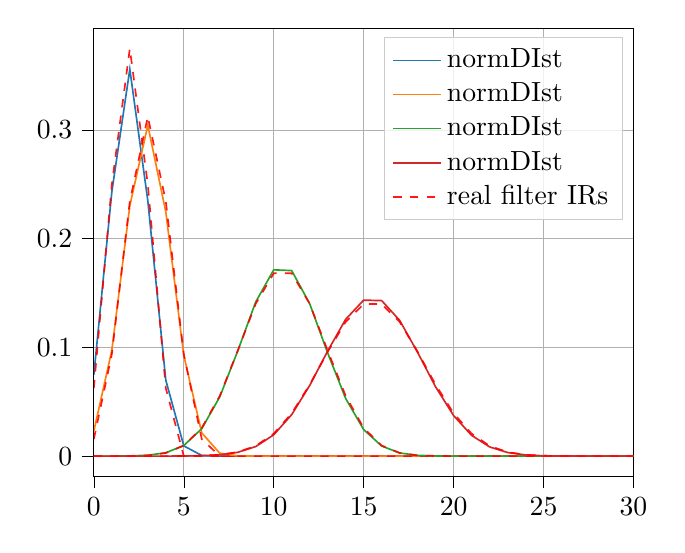
\begin{tikzpicture}

\definecolor{color0}{rgb}{0.1216,0.4667,0.7059}
\definecolor{color1}{rgb}{1.0000,0.4980,0.0549}
\definecolor{color2}{rgb}{0.1725,0.6275,0.1725}
\definecolor{color3}{rgb}{0.8392,0.1529,0.1569}

\begin{axis}[
legend cell align={left},
legend style={fill opacity=0.8, draw opacity=1, text opacity=1, draw=white!80.0000!black},
tick align=outside,
tick pos=left,
x grid style={white!69.0196!black},
xmajorgrids,
xmin=0.0000, xmax=30.0000,
xtick style={color=black},
y grid style={white!69.0196!black},
ymajorgrids,
ymin=-0.0188, ymax=0.3937,
ytick style={color=black}
]
\addplot [semithick, color0]
table {%
0.0000 0.0749
1.0000 0.2432
2.0000 0.3560
3.0000 0.2350
4.0000 0.0699
5.0000 0.0094
6.0000 0.0006
7.0000 0.0000
8.0000 0.0000
9.0000 0.0000
10.0000 0.0000
11.0000 0.0000
12.0000 0.0000
13.0000 0.0000
14.0000 0.0000
15.0000 0.0000
16.0000 0.0000
17.0000 0.0000
18.0000 0.0000
19.0000 0.0000
20.0000 0.0000
21.0000 0.0000
22.0000 0.0000
23.0000 0.0000
24.0000 0.0000
25.0000 0.0000
26.0000 0.0000
27.0000 0.0000
28.0000 0.0000
29.0000 0.0000
30.0000 0.0000
31.0000 0.0000
32.0000 0.0000
33.0000 0.0000
34.0000 0.0000
35.0000 0.0000
36.0000 0.0000
37.0000 0.0000
38.0000 0.0000
39.0000 0.0000
40.0000 0.0000
41.0000 0.0000
42.0000 0.0000
43.0000 0.0000
44.0000 0.0000
45.0000 0.0000
46.0000 0.0000
47.0000 0.0000
48.0000 0.0000
49.0000 0.0000
50.0000 0.0000
51.0000 0.0000
52.0000 0.0000
53.0000 0.0000
54.0000 0.0000
55.0000 0.0000
56.0000 0.0000
57.0000 0.0000
58.0000 0.0000
59.0000 0.0000
60.0000 0.0000
61.0000 0.0000
62.0000 0.0000
63.0000 0.0000
64.0000 0.0000
65.0000 0.0000
66.0000 0.0000
67.0000 0.0000
68.0000 0.0000
69.0000 0.0000
70.0000 0.0000
71.0000 0.0000
72.0000 0.0000
73.0000 0.0000
74.0000 0.0000
75.0000 0.0000
76.0000 0.0000
77.0000 0.0000
78.0000 0.0000
79.0000 0.0000
80.0000 0.0000
81.0000 0.0000
82.0000 0.0000
83.0000 0.0000
84.0000 0.0000
85.0000 0.0000
86.0000 0.0000
87.0000 0.0000
88.0000 0.0000
89.0000 0.0000
90.0000 0.0000
91.0000 0.0000
92.0000 0.0000
93.0000 0.0000
94.0000 0.0000
95.0000 0.0000
96.0000 0.0000
97.0000 0.0000
98.0000 0.0000
99.0000 0.0000
};
\addlegendentry{normDIst}
\addplot [semithick, red, opacity=0.9, dashed, forget plot]
table {%
0.0000 0.0625
1.0000 0.2500
2.0000 0.3750
3.0000 0.2500
4.0000 0.0625
5.0000 0.0000
6.0000 0.0000
7.0000 0.0000
8.0000 0.0000
9.0000 0.0000
10.0000 0.0000
11.0000 0.0000
12.0000 0.0000
13.0000 0.0000
14.0000 0.0000
15.0000 0.0000
16.0000 0.0000
17.0000 0.0000
18.0000 0.0000
19.0000 0.0000
20.0000 0.0000
21.0000 0.0000
22.0000 0.0000
23.0000 0.0000
24.0000 0.0000
25.0000 0.0000
26.0000 0.0000
27.0000 0.0000
28.0000 0.0000
29.0000 0.0000
30.0000 0.0000
31.0000 0.0000
32.0000 0.0000
33.0000 0.0000
34.0000 0.0000
35.0000 0.0000
36.0000 0.0000
37.0000 0.0000
38.0000 0.0000
39.0000 0.0000
40.0000 0.0000
41.0000 0.0000
42.0000 0.0000
43.0000 0.0000
44.0000 0.0000
45.0000 0.0000
46.0000 0.0000
47.0000 0.0000
48.0000 0.0000
49.0000 0.0000
50.0000 0.0000
51.0000 0.0000
52.0000 0.0000
53.0000 0.0000
54.0000 0.0000
55.0000 0.0000
56.0000 0.0000
57.0000 0.0000
58.0000 0.0000
59.0000 0.0000
60.0000 0.0000
61.0000 0.0000
62.0000 0.0000
63.0000 0.0000
64.0000 0.0000
65.0000 0.0000
66.0000 0.0000
67.0000 0.0000
68.0000 0.0000
69.0000 0.0000
70.0000 0.0000
71.0000 0.0000
72.0000 0.0000
73.0000 0.0000
74.0000 0.0000
75.0000 0.0000
76.0000 0.0000
77.0000 0.0000
78.0000 0.0000
79.0000 0.0000
80.0000 0.0000
81.0000 0.0000
82.0000 0.0000
83.0000 0.0000
84.0000 0.0000
85.0000 0.0000
86.0000 0.0000
87.0000 0.0000
88.0000 0.0000
89.0000 0.0000
90.0000 0.0000
91.0000 0.0000
92.0000 0.0000
93.0000 0.0000
94.0000 0.0000
95.0000 0.0000
96.0000 0.0000
97.0000 0.0000
98.0000 0.0000
99.0000 0.0000
};
\addplot [semithick, color1]
table {%
0.0000 0.0230
1.0000 0.0974
2.0000 0.2304
3.0000 0.3044
4.0000 0.2247
5.0000 0.0926
6.0000 0.0213
7.0000 0.0027
8.0000 0.0002
9.0000 0.0000
10.0000 0.0000
11.0000 0.0000
12.0000 0.0000
13.0000 0.0000
14.0000 0.0000
15.0000 0.0000
16.0000 0.0000
17.0000 0.0000
18.0000 0.0000
19.0000 0.0000
20.0000 0.0000
21.0000 0.0000
22.0000 0.0000
23.0000 0.0000
24.0000 0.0000
25.0000 0.0000
26.0000 0.0000
27.0000 0.0000
28.0000 0.0000
29.0000 0.0000
30.0000 0.0000
31.0000 0.0000
32.0000 0.0000
33.0000 0.0000
34.0000 0.0000
35.0000 0.0000
36.0000 0.0000
37.0000 0.0000
38.0000 0.0000
39.0000 0.0000
40.0000 0.0000
41.0000 0.0000
42.0000 0.0000
43.0000 0.0000
44.0000 0.0000
45.0000 0.0000
46.0000 0.0000
47.0000 0.0000
48.0000 0.0000
49.0000 0.0000
50.0000 0.0000
51.0000 0.0000
52.0000 0.0000
53.0000 0.0000
54.0000 0.0000
55.0000 0.0000
56.0000 0.0000
57.0000 0.0000
58.0000 0.0000
59.0000 0.0000
60.0000 0.0000
61.0000 0.0000
62.0000 0.0000
63.0000 0.0000
64.0000 0.0000
65.0000 0.0000
66.0000 0.0000
67.0000 0.0000
68.0000 0.0000
69.0000 0.0000
70.0000 0.0000
71.0000 0.0000
72.0000 0.0000
73.0000 0.0000
74.0000 0.0000
75.0000 0.0000
76.0000 0.0000
77.0000 0.0000
78.0000 0.0000
79.0000 0.0000
80.0000 0.0000
81.0000 0.0000
82.0000 0.0000
83.0000 0.0000
84.0000 0.0000
85.0000 0.0000
86.0000 0.0000
87.0000 0.0000
88.0000 0.0000
89.0000 0.0000
90.0000 0.0000
91.0000 0.0000
92.0000 0.0000
93.0000 0.0000
94.0000 0.0000
95.0000 0.0000
96.0000 0.0000
97.0000 0.0000
98.0000 0.0000
99.0000 0.0000
};
\addlegendentry{normDIst}
\addplot [semithick, red, opacity=0.9, dashed, forget plot]
table {%
0.0000 0.0156
1.0000 0.0938
2.0000 0.2344
3.0000 0.3125
4.0000 0.2344
5.0000 0.0938
6.0000 0.0156
7.0000 0.0000
8.0000 0.0000
9.0000 0.0000
10.0000 0.0000
11.0000 0.0000
12.0000 0.0000
13.0000 0.0000
14.0000 0.0000
15.0000 0.0000
16.0000 0.0000
17.0000 0.0000
18.0000 0.0000
19.0000 0.0000
20.0000 0.0000
21.0000 0.0000
22.0000 0.0000
23.0000 0.0000
24.0000 0.0000
25.0000 0.0000
26.0000 0.0000
27.0000 0.0000
28.0000 0.0000
29.0000 0.0000
30.0000 0.0000
31.0000 0.0000
32.0000 0.0000
33.0000 0.0000
34.0000 0.0000
35.0000 0.0000
36.0000 0.0000
37.0000 0.0000
38.0000 0.0000
39.0000 0.0000
40.0000 0.0000
41.0000 0.0000
42.0000 0.0000
43.0000 0.0000
44.0000 0.0000
45.0000 0.0000
46.0000 0.0000
47.0000 0.0000
48.0000 0.0000
49.0000 0.0000
50.0000 0.0000
51.0000 0.0000
52.0000 0.0000
53.0000 0.0000
54.0000 0.0000
55.0000 0.0000
56.0000 0.0000
57.0000 0.0000
58.0000 0.0000
59.0000 0.0000
60.0000 0.0000
61.0000 0.0000
62.0000 0.0000
63.0000 0.0000
64.0000 0.0000
65.0000 0.0000
66.0000 0.0000
67.0000 0.0000
68.0000 0.0000
69.0000 0.0000
70.0000 0.0000
71.0000 0.0000
72.0000 0.0000
73.0000 0.0000
74.0000 0.0000
75.0000 0.0000
76.0000 0.0000
77.0000 0.0000
78.0000 0.0000
79.0000 0.0000
80.0000 0.0000
81.0000 0.0000
82.0000 0.0000
83.0000 0.0000
84.0000 0.0000
85.0000 0.0000
86.0000 0.0000
87.0000 0.0000
88.0000 0.0000
89.0000 0.0000
90.0000 0.0000
91.0000 0.0000
92.0000 0.0000
93.0000 0.0000
94.0000 0.0000
95.0000 0.0000
96.0000 0.0000
97.0000 0.0000
98.0000 0.0000
99.0000 0.0000
};
\addplot [semithick, color2]
table {%
0.0000 0.0000
1.0000 0.0000
2.0000 0.0002
3.0000 0.0008
4.0000 0.0031
5.0000 0.0097
6.0000 0.0253
7.0000 0.0545
8.0000 0.0968
9.0000 0.1419
10.0000 0.1714
11.0000 0.1707
12.0000 0.1402
13.0000 0.0949
14.0000 0.0530
15.0000 0.0244
16.0000 0.0093
17.0000 0.0029
18.0000 0.0007
19.0000 0.0002
20.0000 0.0000
21.0000 0.0000
22.0000 0.0000
23.0000 0.0000
24.0000 0.0000
25.0000 0.0000
26.0000 0.0000
27.0000 0.0000
28.0000 0.0000
29.0000 0.0000
30.0000 0.0000
31.0000 0.0000
32.0000 0.0000
33.0000 0.0000
34.0000 0.0000
35.0000 0.0000
36.0000 0.0000
37.0000 0.0000
38.0000 0.0000
39.0000 0.0000
40.0000 0.0000
41.0000 0.0000
42.0000 0.0000
43.0000 0.0000
44.0000 0.0000
45.0000 0.0000
46.0000 0.0000
47.0000 0.0000
48.0000 0.0000
49.0000 0.0000
50.0000 0.0000
51.0000 0.0000
52.0000 0.0000
53.0000 0.0000
54.0000 0.0000
55.0000 0.0000
56.0000 0.0000
57.0000 0.0000
58.0000 0.0000
59.0000 0.0000
60.0000 0.0000
61.0000 0.0000
62.0000 0.0000
63.0000 0.0000
64.0000 0.0000
65.0000 0.0000
66.0000 0.0000
67.0000 0.0000
68.0000 0.0000
69.0000 0.0000
70.0000 0.0000
71.0000 0.0000
72.0000 0.0000
73.0000 0.0000
74.0000 0.0000
75.0000 0.0000
76.0000 0.0000
77.0000 0.0000
78.0000 0.0000
79.0000 0.0000
80.0000 0.0000
81.0000 0.0000
82.0000 0.0000
83.0000 0.0000
84.0000 0.0000
85.0000 0.0000
86.0000 0.0000
87.0000 0.0000
88.0000 0.0000
89.0000 0.0000
90.0000 0.0000
91.0000 0.0000
92.0000 0.0000
93.0000 0.0000
94.0000 0.0000
95.0000 0.0000
96.0000 0.0000
97.0000 0.0000
98.0000 0.0000
99.0000 0.0000
};
\addlegendentry{normDIst}
\addplot [semithick, red, opacity=0.9, dashed, forget plot]
table {%
0.0000 0.0000
1.0000 0.0000
2.0000 0.0001
3.0000 0.0006
4.0000 0.0029
5.0000 0.0097
6.0000 0.0259
7.0000 0.0554
8.0000 0.0970
9.0000 0.1402
10.0000 0.1682
11.0000 0.1682
12.0000 0.1402
13.0000 0.0970
14.0000 0.0554
15.0000 0.0259
16.0000 0.0097
17.0000 0.0029
18.0000 0.0006
19.0000 0.0001
20.0000 0.0000
21.0000 0.0000
22.0000 0.0000
23.0000 0.0000
24.0000 0.0000
25.0000 0.0000
26.0000 0.0000
27.0000 0.0000
28.0000 0.0000
29.0000 0.0000
30.0000 0.0000
31.0000 0.0000
32.0000 0.0000
33.0000 0.0000
34.0000 0.0000
35.0000 0.0000
36.0000 0.0000
37.0000 0.0000
38.0000 0.0000
39.0000 0.0000
40.0000 0.0000
41.0000 0.0000
42.0000 0.0000
43.0000 0.0000
44.0000 0.0000
45.0000 0.0000
46.0000 0.0000
47.0000 0.0000
48.0000 0.0000
49.0000 0.0000
50.0000 0.0000
51.0000 0.0000
52.0000 0.0000
53.0000 0.0000
54.0000 0.0000
55.0000 0.0000
56.0000 0.0000
57.0000 0.0000
58.0000 0.0000
59.0000 0.0000
60.0000 0.0000
61.0000 0.0000
62.0000 0.0000
63.0000 0.0000
64.0000 0.0000
65.0000 0.0000
66.0000 0.0000
67.0000 0.0000
68.0000 0.0000
69.0000 0.0000
70.0000 0.0000
71.0000 0.0000
72.0000 0.0000
73.0000 0.0000
74.0000 0.0000
75.0000 0.0000
76.0000 0.0000
77.0000 0.0000
78.0000 0.0000
79.0000 0.0000
80.0000 0.0000
81.0000 0.0000
82.0000 0.0000
83.0000 0.0000
84.0000 0.0000
85.0000 0.0000
86.0000 0.0000
87.0000 0.0000
88.0000 0.0000
89.0000 0.0000
90.0000 0.0000
91.0000 0.0000
92.0000 0.0000
93.0000 0.0000
94.0000 0.0000
95.0000 0.0000
96.0000 0.0000
97.0000 0.0000
98.0000 0.0000
99.0000 0.0000
};
\addplot [semithick, color3]
table {%
0.0000 0.0000
1.0000 0.0000
2.0000 0.0000
3.0000 0.0000
4.0000 0.0000
5.0000 0.0001
6.0000 0.0004
7.0000 0.0012
8.0000 0.0035
9.0000 0.0088
10.0000 0.0196
11.0000 0.0382
12.0000 0.0650
13.0000 0.0967
14.0000 0.1259
15.0000 0.1435
16.0000 0.1431
17.0000 0.1249
18.0000 0.0954
19.0000 0.0637
20.0000 0.0373
21.0000 0.0191
22.0000 0.0085
23.0000 0.0033
24.0000 0.0011
25.0000 0.0003
26.0000 0.0001
27.0000 0.0000
28.0000 0.0000
29.0000 0.0000
30.0000 0.0000
31.0000 0.0000
32.0000 0.0000
33.0000 0.0000
34.0000 0.0000
35.0000 0.0000
36.0000 0.0000
37.0000 0.0000
38.0000 0.0000
39.0000 0.0000
40.0000 0.0000
41.0000 0.0000
42.0000 0.0000
43.0000 0.0000
44.0000 0.0000
45.0000 0.0000
46.0000 0.0000
47.0000 0.0000
48.0000 0.0000
49.0000 0.0000
50.0000 0.0000
51.0000 0.0000
52.0000 0.0000
53.0000 0.0000
54.0000 0.0000
55.0000 0.0000
56.0000 0.0000
57.0000 0.0000
58.0000 0.0000
59.0000 0.0000
60.0000 0.0000
61.0000 0.0000
62.0000 0.0000
63.0000 0.0000
64.0000 0.0000
65.0000 0.0000
66.0000 0.0000
67.0000 0.0000
68.0000 0.0000
69.0000 0.0000
70.0000 0.0000
71.0000 0.0000
72.0000 0.0000
73.0000 0.0000
74.0000 0.0000
75.0000 0.0000
76.0000 0.0000
77.0000 0.0000
78.0000 0.0000
79.0000 0.0000
80.0000 0.0000
81.0000 0.0000
82.0000 0.0000
83.0000 0.0000
84.0000 0.0000
85.0000 0.0000
86.0000 0.0000
87.0000 0.0000
88.0000 0.0000
89.0000 0.0000
90.0000 0.0000
91.0000 0.0000
92.0000 0.0000
93.0000 0.0000
94.0000 0.0000
95.0000 0.0000
96.0000 0.0000
97.0000 0.0000
98.0000 0.0000
99.0000 0.0000
};
\addlegendentry{normDIst}
\addplot [semithick, red, opacity=0.9, dashed]
table {%
0.0000 0.0000
1.0000 0.0000
2.0000 0.0000
3.0000 0.0000
4.0000 0.0000
5.0000 0.0001
6.0000 0.0003
7.0000 0.0012
8.0000 0.0037
9.0000 0.0094
10.0000 0.0207
11.0000 0.0394
12.0000 0.0657
13.0000 0.0960
14.0000 0.1235
15.0000 0.1399
16.0000 0.1399
17.0000 0.1235
18.0000 0.0960
19.0000 0.0657
20.0000 0.0394
21.0000 0.0207
22.0000 0.0094
23.0000 0.0037
24.0000 0.0012
25.0000 0.0003
26.0000 0.0001
27.0000 0.0000
28.0000 0.0000
29.0000 0.0000
30.0000 0.0000
31.0000 0.0000
32.0000 0.0000
33.0000 0.0000
34.0000 0.0000
35.0000 0.0000
36.0000 0.0000
37.0000 0.0000
38.0000 0.0000
39.0000 0.0000
40.0000 0.0000
41.0000 0.0000
42.0000 0.0000
43.0000 0.0000
44.0000 0.0000
45.0000 0.0000
46.0000 0.0000
47.0000 0.0000
48.0000 0.0000
49.0000 0.0000
50.0000 0.0000
51.0000 0.0000
52.0000 0.0000
53.0000 0.0000
54.0000 0.0000
55.0000 0.0000
56.0000 0.0000
57.0000 0.0000
58.0000 0.0000
59.0000 0.0000
60.0000 0.0000
61.0000 0.0000
62.0000 0.0000
63.0000 0.0000
64.0000 0.0000
65.0000 0.0000
66.0000 0.0000
67.0000 0.0000
68.0000 0.0000
69.0000 0.0000
70.0000 0.0000
71.0000 0.0000
72.0000 0.0000
73.0000 0.0000
74.0000 0.0000
75.0000 0.0000
76.0000 0.0000
77.0000 0.0000
78.0000 0.0000
79.0000 0.0000
80.0000 0.0000
81.0000 0.0000
82.0000 0.0000
83.0000 0.0000
84.0000 0.0000
85.0000 0.0000
86.0000 0.0000
87.0000 0.0000
88.0000 0.0000
89.0000 0.0000
90.0000 0.0000
91.0000 0.0000
92.0000 0.0000
93.0000 0.0000
94.0000 0.0000
95.0000 0.0000
96.0000 0.0000
97.0000 0.0000
98.0000 0.0000
99.0000 0.0000
};
\addlegendentry{real filter IRs}
\end{axis}

\end{tikzpicture}

%         % % This file was created by tikzplotlib v0.9.1.
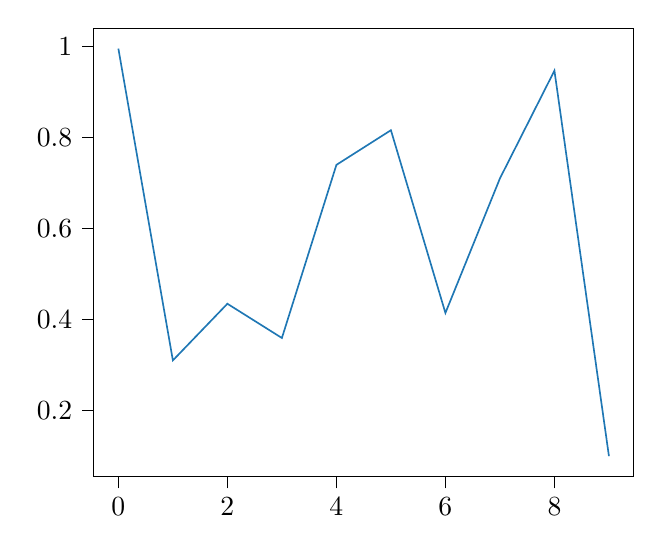
\begin{tikzpicture}

\definecolor{color0}{rgb}{0.12156862745098,0.466666666666667,0.705882352941177}

\begin{axis}[
tick align=outside,
tick pos=left,
x grid style={white!69.0196078431373!black},
xmin=-0.45, xmax=9.45,
xtick style={color=black},
y grid style={white!69.0196078431373!black},
ymin=0.0547180265499415, ymax=1.04072818407209,
ytick style={color=black}
]
\addplot [semithick, color0]
table {%
0 0.995909540548354
1 0.31012840026619
2 0.434725290951576
3 0.359411361369715
4 0.740164470332283
5 0.816417637366752
6 0.41448343483885
7 0.710390394064541
8 0.947408418028086
9 0.0995366700736754
};
\end{axis}

\end{tikzpicture}

%     \end{center}
%     \caption{A PGF histogram from \texttt{matplotlib}.}
% \end{figure}


% Advantage of compute shader.
% Maybe introduce cascaded Lowpass.



% All figures should be centred on the column (or page, if the figure spans both columns).
% Figure captions (in italic) should follow each figure and have the format given in Figure \ref{fft_plot}.
% %
% Vectorial figures are preferred. For example when using
% \texttt{Matlab}, export using either Postscript or PDF format. Also,
% in order to provide a better readability, figure text font size
% should be at least identical to footnote font size. To do so using
% \texttt{Matlab}, use the \texttt{subplot} command before plotting.
% If bitmap figures are used, please make sure that the resolution is
% enough for print quality. Fig. \ref{ftt_plot2} illustrates an
% example of a figure spanning two columns.
%


% \begin{figure}
%     \begin{center}
%       \input{img/spec1}
%     \end{center}
%     \caption{\label{fig:shoe} \it Spec by this approach. Impulse response of shoebox room. Computed using the proposed method and \cite{lehmann_fast_2020}. }
    
% \end{figure}



% \begin{figure}
%     \begin{center}
%       \input{img/orig}
%     \end{center}
%     \caption{\label{fig:shoe} \it Spec by matlab. Impulse response of shoebox room. Computed using the proposed method and \cite{lehmann_fast_2020}. }
    
% \end{figure}


% \begin{figure}
%     \begin{center}
%       % This file was created by tikzplotlib v0.9.1.
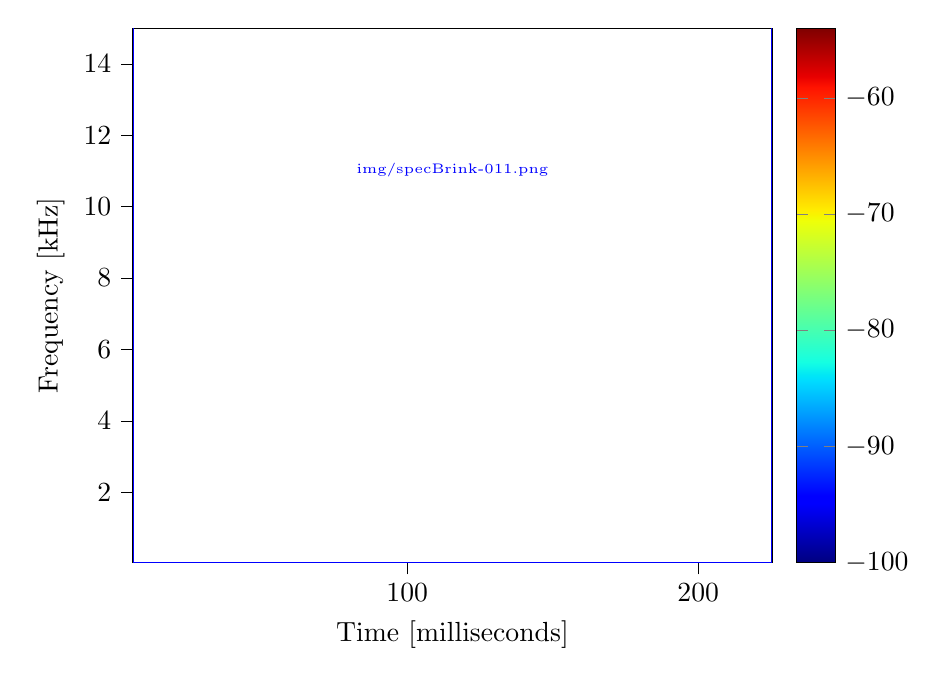
\begin{tikzpicture}

\begin{axis}[
colorbar,
colorbar style={ylabel={}, y label style={yshift=1.5em}},
colormap={mymap}{[1pt]
  rgb(0pt)=(0.0000,0.0000,0.5000);
  rgb(22pt)=(0.0000,0.0000,1.0000);
  rgb(25pt)=(0.0000,0.0000,1.0000);
  rgb(68pt)=(0.0000,0.8600,1.0000);
  rgb(70pt)=(0.0000,0.9000,0.9677);
  rgb(75pt)=(0.0806,1.0000,0.8871);
  rgb(128pt)=(0.9355,1.0000,0.0323);
  rgb(130pt)=(0.9677,0.9630,0.0000);
  rgb(132pt)=(1.0000,0.9259,0.0000);
  rgb(178pt)=(1.0000,0.0741,0.0000);
  rgb(182pt)=(0.9091,0.0000,0.0000);
  rgb(200pt)=(0.5000,0.0000,0.0000)
},
point meta max=-54.0062,
point meta min=-100.0000,
tick align=outside,
tick pos=left,
width=0.8\textwidth,
x grid style={white!69.0196!black},
xlabel={Time [milliseconds]},
xmin=0005.7, xmax=225.4,xtick={0, 100,200},
xtick style={color=black},
y grid style={white!69.0196!black},
ylabel={Frequency [kHz]},
ymin=0.0300000, ymax=15.0000000,
ytick style={color=black}
]
\addplot graphics [includegraphics cmd=\pgfimage,xmin=5.7, xmax=225.4, ymin=0.0000, ymax=22.0500000] {img/specBrink-011.png};
\end{axis}

\end{tikzpicture}

%     \end{center}
%     \caption{\label{fig:shoe} \it Original \cite{brinkmann_round_2019}. }
    
% \end{figure}


% \begin{figure}
%     \begin{center}
%       % This file was created by tikzplotlib v0.9.1.
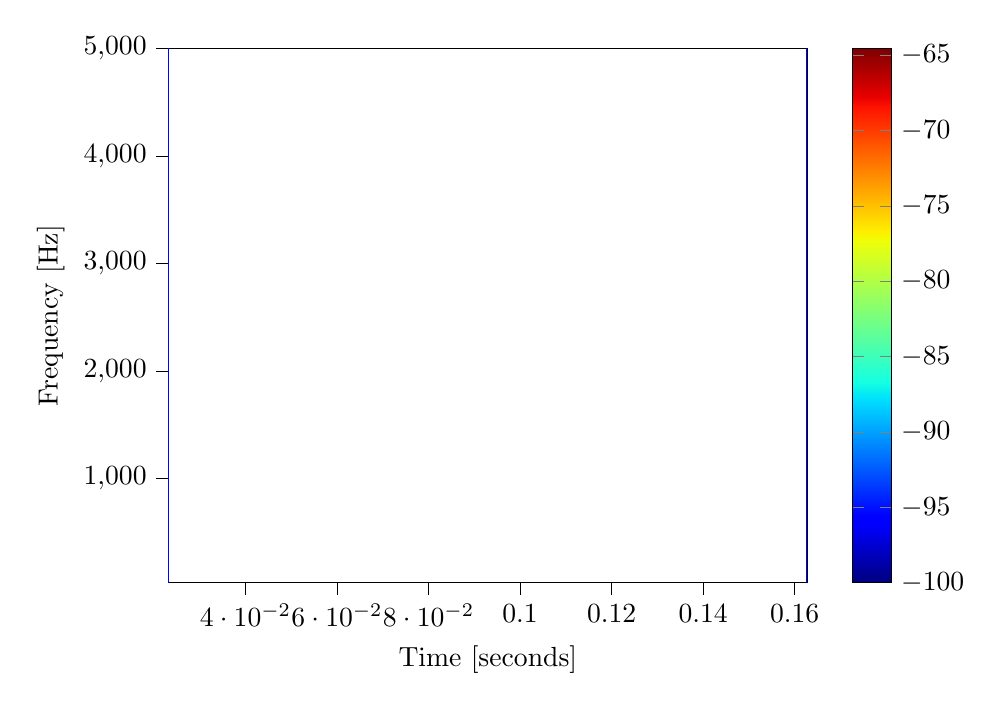
\begin{tikzpicture}

\begin{axis}[
colorbar,
colorbar style={ylabel={}},
colormap={mymap}{[1pt]
  rgb(0pt)=(0.0000,0.0000,0.5000);
  rgb(22pt)=(0.0000,0.0000,1.0000);
  rgb(25pt)=(0.0000,0.0000,1.0000);
  rgb(68pt)=(0.0000,0.8600,1.0000);
  rgb(70pt)=(0.0000,0.9000,0.9677);
  rgb(75pt)=(0.0806,1.0000,0.8871);
  rgb(128pt)=(0.9355,1.0000,0.0323);
  rgb(130pt)=(0.9677,0.9630,0.0000);
  rgb(132pt)=(1.0000,0.9259,0.0000);
  rgb(178pt)=(1.0000,0.0741,0.0000);
  rgb(182pt)=(0.9091,0.0000,0.0000);
  rgb(200pt)=(0.5000,0.0000,0.0000)
},
point meta max=-64.5644,
point meta min=-100.0000,
tick align=outside,
tick pos=left,
width=0.8\textwidth,
x grid style={white!69.0196!black},
xlabel={Time [seconds]},
xmin=0.0231, xmax=0.1628,
xtick style={color=black},
y grid style={white!69.0196!black},
ylabel={Frequency [Hz]},
ymin=30.0000, ymax=5000.0000,
ytick style={color=black}
]
\addplot graphics [includegraphics cmd=\pgfimage,xmin=0.0231, xmax=0.1628, ymin=0.0000, ymax=22050.0000] {img/simBrink-007.png};
\end{axis}

\end{tikzpicture}

%     \end{center}
%     \caption{\label{fig:shoe} \it Simulated. }
    
% \end{figure}

% \begin{enumerate}



% Eric A. Lehmann (2020). Fast simulation of acoustic room impulse responses (image-source method) (https://www.mathworks.com/matlabcentral/fileexchange/25965-fast-simulation-of-acoustic-room-impulse-responses-image-source-method), MATLAB Central File Exchange. Retrieved February 14, 2020.

% \end{enumerate}


% \begin{figure}[ht]
% \centerline{\includegraphics[scale=0.8]{fft_plot2}}
% \caption{\label{fft_plot}{\it Sinusoid in time and frequency domain. Short captions are centred, long captions (more than 1 line) are justified.}}
% \end{figure}
% %
% \begin{figure*}[ht]
% \center
% \includegraphics[width=5in]{TwoColumnSine2}
% \caption{\label{ftt_plot2}{\it A figure spanning two columns, as mentioned in Sec. . }}
% \end{figure*}


% \begin{figure}[ht]
% \centerline{\includegraphics[scale=0.8]{img/test1.pgf}}
% \caption{\label{fft_plot}{\it Sinusoid in time and frequency domain. Short captions are centred, long captions (more than 1 line) are justified.}}
% \end{figure}

% \begin{figure}
%     \begin{center}
%       % This file was created by tikzplotlib v0.9.1.
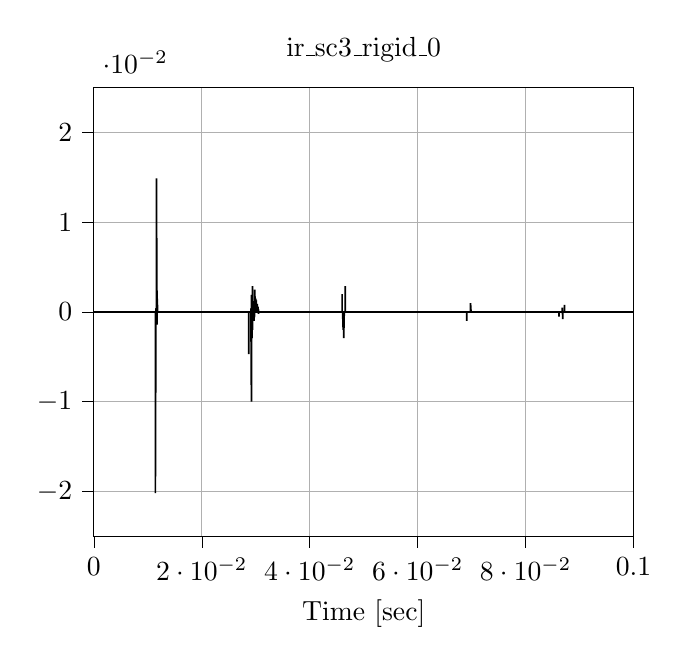
\begin{tikzpicture}

\begin{axis}[
tick align=outside,
tick pos=left,
title={ir\_sc3\_rigid\_0},
x grid style={white!69.0196!black},
xlabel={Time [sec]},
xmajorgrids,
xmin=0.0000, xmax=0.1000,
xtick style={color=black},
y grid style={white!69.0196!black},
ymajorgrids,
ymin=-0.0250, ymax=0.0250,
ytick style={color=black}
]
\addplot [semithick, black]
table {%
0.0000 0.0000
0.0114 0.0000
0.0114 -0.0202
0.0115 0.0000
0.0115 0.0000
0.0115 0.0000
0.0115 0.0001
0.0116 0.0000
0.0116 0.0001
0.0116 0.0149
0.0117 -0.0014
0.0117 0.0024
0.0117 0.0003
0.0117 0.0020
0.0118 0.0005
0.0118 0.0000
0.0121 0.0000
0.0287 0.0000
0.0287 -0.0047
0.0287 0.0000
0.0291 0.0000
0.0291 0.0004
0.0292 -0.0100
0.0292 0.0019
0.0292 -0.0009
0.0292 -0.0006
0.0293 0.0004
0.0293 -0.0001
0.0293 -0.0000
0.0293 0.0004
0.0293 -0.0029
0.0294 0.0029
0.0294 -0.0020
0.0294 0.0018
0.0295 -0.0001
0.0295 0.0000
0.0295 0.0009
0.0295 -0.0009
0.0295 0.0012
0.0296 -0.0004
0.0296 0.0000
0.0296 -0.0005
0.0297 0.0010
0.0297 -0.0010
0.0297 0.0011
0.0297 -0.0008
0.0298 0.0013
0.0298 -0.0005
0.0298 0.0025
0.0299 0.0009
0.0299 0.0012
0.0299 0.0007
0.0300 0.0011
0.0300 0.0007
0.0300 -0.0001
0.0300 0.0015
0.0300 0.0005
0.0301 0.0007
0.0301 0.0004
0.0301 0.0008
0.0302 0.0004
0.0302 0.0008
0.0302 0.0002
0.0302 0.0007
0.0303 0.0006
0.0303 -0.0001
0.0303 0.0009
0.0303 -0.0000
0.0304 0.0006
0.0304 0.0004
0.0304 0.0000
0.0304 0.0006
0.0305 -0.0002
0.0305 0.0003
0.0305 0.0000
0.0460 0.0000
0.0460 0.0020
0.0460 -0.0000
0.0461 -0.0000
0.0462 -0.0020
0.0462 0.0000
0.0463 0.0000
0.0463 -0.0029
0.0464 -0.0000
0.0465 0.0000
0.0466 0.0000
0.0466 0.0029
0.0466 0.0000
0.0691 0.0000
0.0691 -0.0010
0.0691 0.0000
0.0698 0.0000
0.0698 0.0010
0.0699 0.0000
0.0862 0.0000
0.0862 -0.0005
0.0862 0.0000
0.0868 0.0000
0.0868 0.0005
0.0869 -0.0008
0.0869 0.0000
0.0872 0.0000
0.0872 0.0008
0.0872 0.0000
0.1000 0.0000
};
\end{axis}

\end{tikzpicture}

%         % % This file was created by tikzplotlib v0.9.1.
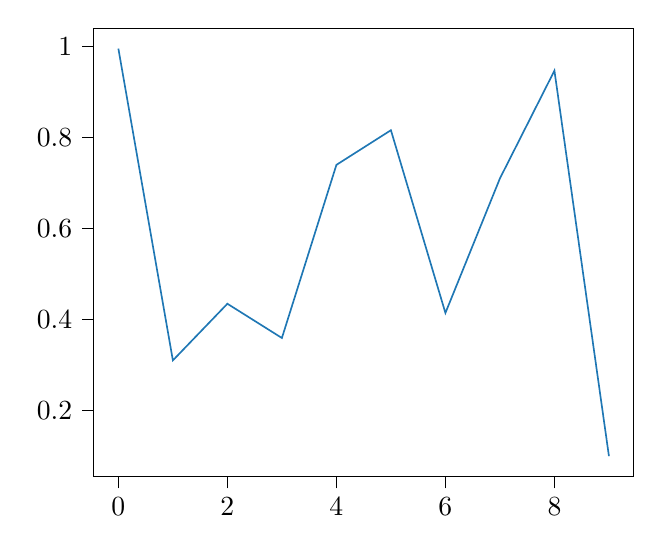
\begin{tikzpicture}

\definecolor{color0}{rgb}{0.12156862745098,0.466666666666667,0.705882352941177}

\begin{axis}[
tick align=outside,
tick pos=left,
x grid style={white!69.0196078431373!black},
xmin=-0.45, xmax=9.45,
xtick style={color=black},
y grid style={white!69.0196078431373!black},
ymin=0.0547180265499415, ymax=1.04072818407209,
ytick style={color=black}
]
\addplot [semithick, color0]
table {%
0 0.995909540548354
1 0.31012840026619
2 0.434725290951576
3 0.359411361369715
4 0.740164470332283
5 0.816417637366752
6 0.41448343483885
7 0.710390394064541
8 0.947408418028086
9 0.0995366700736754
};
\end{axis}

\end{tikzpicture}

%     \end{center}
%     \caption{A PGF histogram from \texttt{matplotlib}.}
% \end{figure}




% \subsection{Tables}
% As for figures, all tables should be centered on the column (or page, if the table spans both columns).
% Table captions should be in italic, precede each table and have the format given in Table \ref{tab:example}.

% \begin{table}[ht]
%   \caption{\itshape Basic trigonometric values.}
%   \centering
%   \begin{tabular}{|c|c|}
%     \hline
%     $\mathrm{angle}\,(\theta, \mathrm{rad})$ & $\sin \theta$ \\\hline
%     $\frac{\pi}{2}$ & $1$ \\
%     $\pi$ & $0$ \\
%     $\frac{3\pi}{2}$ & $-1$ \\
%     $2\pi$ & $0$ \\\hline
%   \end{tabular}
%   %
%   \label{tab:example}
% \end{table}

% \begin{table*}[ht]
%   \caption{{\it Basic trigonometric values, spanning two columns.}}
%   \centering
%   \begin{tabular}{|c|c|c|c|c|c|c|}\hline
%     $\mathrm{angle}\, (\theta, \mathrm{rad})$ & $\sin \theta$ & $\cos \theta $ & $(\sin \theta)/2 $ & $(\cos \theta) /2 $ & $(\sin \theta)/3 $ & $(\cos \theta)/3$    \\\hline
%     $\frac{\pi}{2}$ & $1$ & $0$ & $1/2$ & $0$ & $1/3$ & $0$ \\
%     $\pi$ & $0$ & $-1$ & $0$ & $-1/2$ & $0$ & $-1/3$\\
%     $\frac{3\pi}{2}$ & $-1$ & $0$ & $-1/2$ & $0$ & $-1/3$ & $0$ \\
%     $2\pi$ & $0$ & $1$ & $0$ & $1/2$ & $0$ & $1/3$ \\\hline
%  \end{tabular}
%   %
%   \label{tab:example2}
% \end{table*}

% \subsection{Equations}
% Equations should be placed on separate lines and numbered:

% \begin{equation}
%   X(e^{j\Omega})=\sum_{n=0}^{N-1}x(n)e^{-j\Omega n}
%   \label{eq1}
%   \end{equation}
%   where the sequence $x(n)$ in equation (\ref{eq1}) is a windowed frame:
%   \begin{equation}
%   x(n)=s(n) w(n)
%   \label{eq2}
% \end{equation}
% %
% with a window function $w(n)$.
